% ------------------------------------------------------------------------
% ------------------------------------------------------------------------
% Modelo de TCC baseado no abnTeX2 para a Universidade Anhembi Morumbi
%
% Configurações iniciais
% ------------------------------------------------------------------------
% ------------------------------------------------------------------------

\documentclass[
	% -- opções da classe memoir --
	12pt,				% tamanho da fonte
	openright,			% capítulos começam em pág ímpar (insere página vazia caso preciso)
	oneside,			% para impressão em recto e verso. Oposto a oneside
	a4paper,			% tamanho do papel. 
	% -- opções da classe abntex2 --
	chapter=TITLE,		% títulos de capítulos convertidos em letras maiúsculas
	%section=TITLE,		% títulos de seções convertidos em letras maiúsculas
	%subsection=TITLE,	% títulos de subseções convertidos em letras maiúsculas
	%subsubsection=TITLE,% títulos de subsubseções convertidos em letras maiúsculas
	% -- opções do pacote babel --
	english,			% idioma adicional para hifenização
	french,				% idioma adicional para hifenização
	spanish,			% idioma adicional para hifenização
	brazil				% o último idioma é o principal do documento
	]{abntex2}

% ---
% PACOTES E CONFIGURAÇÕES 
% ---

% \usepackage[usenames,dvipsnames]{pstricks}
% \usepackage{epsfig}
% \usepackage{pst-grad} % For gradients
% \usepackage{pst-plot} % For axes
% \usepackage[space]{grffile} % For spaces in paths
% \usepackage{etoolbox} % For spaces in paths
% \makeatletter % For spaces in paths
% \patchcmd\Gread@eps{\@inputcheck#1 }{\@inputcheck"#1"\relax}{}{}
% \makeatother


% --- Fontes ---
\usepackage[utf8]{inputenc}		% Codificação do documento (conversão automática dos acentos)
\usepackage{times}			    % Usa a fonte Nimbus Roman (clone da Times New Roman)
\usepackage{courier}		    % Courier para fontes monoespaçadas
\usepackage{mathptmx}           % Suporte à notação matemática com Nimbus Roman
\usepackage[T1]{fontenc}		% Selecao de codigos de fonte.
  \renewcommand{\sfdefault}{\rmdefault} % Títulos e texto com a mesma fonte serifada
%\usepackage{fontspec}          % Para usar a fonte Times New Roman, comente as 4 linhas acima,
%\setmainfont{Times New Roman}  % mas fique avisado que não fica muito bom.
% --- /Fontes ---

\usepackage{lastpage}			% Usado pela Ficha catalográfica
\usepackage{float}			% Usado pela Ficha catalográfica
\usepackage{indentfirst}		% Indenta o primeiro parágrafo de cada seção.
\usepackage{color}				% Controle das cores
\usepackage{graphicx}			% Inclusão de elementos gráficos
  \graphicspath{ {img/} }   % Define o diretório das imagens
%\usepackage{epsfig}            % Incluir Postscript encapsulado (prefira o graphicx)
\usepackage{microtype} 			% Melhorias de justificação
\usepackage{textgreek}          % Suporte a letras gregas
\usepackage{nicefrac}           % Frações na linha
\usepackage{tabulary}           % Ambiente de tabelas
\usepackage{amsmath}            % Melhorias tipográficas para escrita matemática
\usepackage{amssymb}            % Mais símbolos matemáticos
\usepackage[export]{adjustbox}  % Para inserir imagens no tamanho máximo disponível, sem escalar
\usepackage{setspace}           % Determina o espaçamento entre linhas
\usepackage{textcomp}
\usepackage{gensymb}            % Símbolos genéricos para modo texto e modo matemático
\usepackage{anhembi-morumbi}    % Customização da capa do TCC para a Anhembi Morumbi
\usepackage{url}                % Verbatim com quebras de linha de URL
\usepackage{booktabs}           % Melhora a qualidade de impressão das tabelas
\usepackage{color}
\usepackage{xcolor}
\usepackage{textcomp}

\definecolor{solarized@base03}{HTML}{002B36}
\definecolor{solarized@base02}{HTML}{073642}
\definecolor{solarized@base01}{HTML}{586e75}
\definecolor{solarized@base00}{HTML}{657b83}
\definecolor{solarized@base0}{HTML}{839496}
\definecolor{solarized@base1}{HTML}{93a1a1}
\definecolor{solarized@base2}{HTML}{EEE8D5}
\definecolor{solarized@base3}{HTML}{FDF6E3}
\definecolor{solarized@yellow}{HTML}{B58900}
\definecolor{solarized@orange}{HTML}{CB4B16}
\definecolor{solarized@red}{HTML}{DC322F}
\definecolor{solarized@magenta}{HTML}{D33682}
\definecolor{solarized@violet}{HTML}{6C71C4}
\definecolor{solarized@blue}{HTML}{268BD2}
\definecolor{solarized@cyan}{HTML}{2AA198}
\definecolor{solarized@green}{HTML}{859900}

\usepackage{listings}           % Para inserir scripts
\lstset{
	language=Scilab, %% Troque para PHP, C, Java, etc... bash é o padrão
	basicstyle=\ttfamily\small,
	numberstyle=\ttfamily\footnotesize,
    upquote=true,
	numbers=left,
	backgroundcolor=\color{gray!10},
	frame=single,
	tabsize=2,
	rulecolor=\color{black!30},
	title=\lstname,
	escapeinside={\%*}{*)},
	breaklines=true,
	breakatwhitespace=true,
	framextopmargin=2pt,
	framexbottommargin=2pt,
	inputencoding=utf8,
	extendedchars=true,
	literate={á}{{\'a}}1 {Á}{{\'A}}1 {ó}{{\'o}}1 {ã}{{\~a}}1 {é}{{\'e}}1 {ç}{{\c{c}}}1 {í}{{\'i}}1 {ê}{{\^}}1,
	keywordstyle=\color{solarized@green},
	stringstyle=\color{solarized@cyan}\ttfamily,
	identifierstyle=\color{solarized@blue},
	commentstyle=\color{solarized@base01},
	emphstyle=\color{solarized@red}
}

%\usepackage{xmpincl}            % Inclua dados de eXtensible Metadata Platform
%  \includexmp{cclicense/metadata} % Template da licença Creative Commons
\usepackage{pdfpages}
%\usepackage[full]{textcomp}    % Suporte para fontes Text Companion
%\usepackage{ifthen}            % Comandos condicionais em documentos LaTeX
%\usepackage{multicol}          % Junta colunas em tabelas
%\usepackage{multirow}          % Junta linhas em tabelas

% --- Pacotes de citações ---
\usepackage{hyperref}           % Links de referências cruzadas
%\usepackage[brazilian,hyperpageref]{backref}	 % Paginas com as citações na bibliografia
\usepackage[alf]{abntex2cite}	% Citações padrão ABNT

  % Configurações do pacote backref
  % Usado sem a opção hyperpageref de backref
%  \renewcommand{\backrefpagesname}{Citado na(s) página(s):~}
  % Texto padrão antes do número das páginas
%  \renewcommand{\backref}{}
  % Define os textos da citação
%  \renewcommand*{\backrefalt}[4]{
 %   \ifcase #1
%	  Nenhuma citação no texto.
%	\or
%	  Citado na página #2.
%	\else
%	  Citado #1 vezes nas páginas #2.
%	\fi}

% --- /Pacotes de citações ---

% --- Pacotes para lista de abreviaturas e siglas e lista de símbolos ---
%% Utilize A para abreviaturas e S para símbolos
\usepackage{nomencl}
  \renewcommand{\nomname}{\listadesiglasname}
\usepackage{etoolbox}

\renewcommand{\nomgroup}[1]{
  \ifstrequal{#1}{S}{
    \cleardoublepage \pretextualchapter{\listadesimbolosname}
  }
}
\makenomenclature
% --- /Pacotes para lista de abreviaturas e siglas e lista de símpolos ---

% --- Inserir gráficos e tabelas dentro de sua própria seção ---
\usepackage[section]{placeins}  % Evita o posicionamento de imagens fora de sua própria seção
  \makeatletter
  \AtBeginDocument{%
    \expandafter\renewcommand\expandafter\subsection\expandafter{%
      \expandafter\@fb@secFB\subsection
    }%
  }
\makeatother
% --- /Inserir gráficos e tabelas dentro de sua própria seção ---

%\renewcommand{\footnotesize}{\small}

% ---
% DADOS DO TRABALHO
% ---
\titulo{Concreto de ultra alto desempenho: introdução, conceitos e aplicações}
\autor{Douglas Araujo de Moura\\ Markus Vinícius Matos Ferreira\\ Daniel Lopes Pereira}
\local{São Paulo}
\data{2017}
\orientador{Msc. Rafaela de Oliveira Amaral}
%\coorientador{Equipe \abnTeX}
\instituicao{Universidade Anhembi Morumbi}
\tipotrabalho{TCC}
% O preambulo deve conter o tipo do trabalho, o objetivo, 
% o nome da instituição e a área de concentração 
\preambulo{Trabalho de Conclusão de Curso apresentado como exigência parcial para a obtenção do título de Graduação do Curso de Engenharia Civil da Universidade Anhembi Morumbi.}
% ---


% ---
% Configurações de aparência do PDF final

% alterando o aspecto da cor azul
\definecolor{blue}{RGB}{41,5,195}

% informações do PDF
\makeatletter
\hypersetup{
     	%pagebackref=true,
		pdftitle={\@title}, 
		pdfauthor={\@author},
    	pdfsubject={\imprimirpreambulo},
	    pdfcreator={LaTeX with abnTeX2},
		pdfkeywords={CUAD} {UHPC} {Ultra High Performance Concrete} {Concreto de Ultra Alto Desempenho} {ponte} {obra de arte} {trabalho acadêmico} {TCC} {engenharia} {engenharia civil}, 
		colorlinks=true,       		% false: boxed links; true: colored links
    	linkcolor=black,          	% color of internal links
    	citecolor=black,        		% color of links to bibliography
    	filecolor=black,      	% color of file links
		urlcolor=black,
		bookmarksdepth=4
}
\makeatother
% --- 

% --- 
% Espaçamentos entre linhas e parágrafos 
% --- 

% O tamanho do parágrafo é dado por:
\setlength{\parindent}{1.3cm}

% Controle do espaçamento entre um parágrafo e outro:
\setlength{\parskip}{0.2cm}  % tente também \onelineskip

% ---
% compila o indice
% ---
\makeindex
% ---

% ----
% Início do documento
% ----
\begin{document}

% Seleciona o idioma do documento (conforme pacotes do babel)
%\selectlanguage{english}
\selectlanguage{brazil}

% Retira espaço extra obsoleto entre as frases.
\frenchspacing 

% ----------------------------------------------------------
% ELEMENTOS PRÉ-TEXTUAIS
% ----------------------------------------------------------
% \pretextual

% ---
% Capa
% ---
\imprimircapa
% ---

% ---
% Folha de rosto
% (o * indica que haverá a ficha bibliográfica)
% ---
\imprimirfolhaderosto
% ---

% ---
% Inserir a ficha bibliografica
% ---

% Isto é um exemplo de Ficha Catalográfica, ou ``Dados internacionais de
% catalogação-na-publicação''. Você pode utilizar este modelo como referência. 
% Porém, provavelmente a biblioteca da sua universidade lhe fornecerá um PDF
% com a ficha catalográfica definitiva após a defesa do trabalho. Quando estiver
% com o documento, salve-o como PDF no diretório do seu projeto e substitua todo
% o conteúdo de implementação deste arquivo pelo comando abaixo:
%
% \begin{fichacatalografica}
%     \includepdf{fig_ficha_catalografica.pdf}
% \end{fichacatalografica}

\begin{fichacatalografica}
	\sffamily
	\vspace*{\fill}					% Posição vertical
	\begin{center}					% Minipage Centralizado
	\fbox{\begin{minipage}[c][8cm]{13.5cm}		% Largura
	\small
	\imprimirautor
	
	\hspace{0.5cm} \imprimirtitulo  / \imprimirautor. --
	\imprimirlocal, \imprimirdata-
	
	\hspace{0.5cm} \pageref{LastPage} p. : il. (algumas color.) ; 30 cm.\\
	
	\hspace{0.5cm} \imprimirorientadorRotulo~\imprimirorientador\\
	
	\hspace{0.5cm}
	\parbox[t]{\textwidth}{\imprimirtipotrabalho~--~\imprimirinstituicao,
	\imprimirdata.}\\
	
	\hspace{0.5cm}
		1. Concreto de ultra alto desempenho.
		2. CUAD.
		I. Ferreira, Markus Vinícius Matos.
		II. Pereira, Daniel Lopes.
		I. Pinheiro, Rafaela Amaral.
		II. \imprimirinstituicao.
		III. Escola de Engenharia e Tecnologia.
		IV. \imprimirtitulo 			
	\end{minipage}}
	\end{center}
\end{fichacatalografica}
% ---

% ---
% Inserir folha de aprovação
% ---

% Isto é um exemplo de Folha de aprovação, elemento obrigatório da NBR
% 14724/2011 (seção 4.2.1.3). Você pode utilizar este modelo até a aprovação
% do trabalho. Após isso, substitua todo o conteúdo deste arquivo por uma
% imagem da página assinada pela banca com o comando abaixo:
%
% \includepdf{folhadeaprovacao_final.pdf}
%
\begin{folhadeaprovacao}

  \begin{center}
    {\ABNTEXchapterfont\large\imprimirautor}

    \vspace*{\fill}\vspace*{\fill}
    \begin{center}
      \ABNTEXchapterfont\bfseries\Large\imprimirtitulo
    \end{center}
    \vspace*{\fill}
    
    \hspace{.45\textwidth}
    \begin{minipage}{.5\textwidth}
        \imprimirpreambulo
    \end{minipage}%
    \vspace*{\fill}
   \end{center}

   \begin{center}
    % Trabalho \line(1,0){100}~em:~\line(1,0){20}~de dezembro de 2017.
      Trabalho aprovado em 9 de dezembro de 2017.
   \end{center}


   \assinatura{\textbf{\imprimirorientador} \\ Orientadora} 
   %\assinatura{\textbf{Drª. Luciana Tiemi Kataoka} \\ Convidado}
   
   %\assinatura{\textbf{Professor} \\ Convidado 2}
   %\assinatura{\textbf{Professor} \\ Convidado 3}
   %\assinatura{\textbf{Professor} \\ Convidado 4}
   
   \vspace{1.5cm}
   \noindent
   Comentários: \line(1,0){394} \\
   \line(1,0){460} \\
   \line(1,0){460} \\
   \line(1,0){460}
      
   \begin{center}
    \vspace*{0.5cm}
    {\large\imprimirlocal}
    \par
    {\large\imprimirdata}
    \vspace*{1cm}
  \end{center}
  
\end{folhadeaprovacao}
% ---

% ---
% Dedicatória
% ---
%\begin{dedicatoria}
%   \vspace*{\fill}
%   \centering
%   \noindent
%   \textit{ Este trabalho é dedicado às crianças adultas que,\\
%   quando pequenas, sonharam em se tornar cientistas.} \vspace*{\fill}
%\end{dedicatoria}
% ---
% ---
% Licença
% ---
%\newpage
%% Copyright (C) 2013 Alexandre Hannud Abdo <abdo@member.fsf.org>
% This work is licensed under the GNU GPL, version 3 or (at your option)
% any later version. A copy of the license can be found here:
% http://www.gnu.org/licenses/gpl

% Copyright (C) 2013 Alexandre Hannud Abdo <abdo@member.fsf.org>
% This work is licensed under the GNU GPL, version 3 or (at your option)
% any later version. A copy of the license can be found here:
% http://www.gnu.org/licenses/gpl

\newcommand{\CcImageCc}[1]{% zoom
	
\includegraphics[#1]{cclicense/media/cc_cc_30}%
}
\newcommand{\CcImageBy}[1]{% zoom
	
\includegraphics[#1]{cclicense/media/cc_by_30}%
}
\newcommand{\CcImageSa}[1]{% zoom
	
\includegraphics[#1]{cclicense/media/cc_sa_30}%
}
\newcommand{\CcGroupBySa}[2]{% zoom, gap
	\CcImageBy{#1}\hspace*{#2}\CcImageSa{#1}%
}


% Copyright (C) 2013 Alexandre Hannud Abdo <abdo@member.fsf.org>
% This work is licensed under the GNU GPL, version 3 or (at your option)
% any later version. A copy of the license can be found here:
% http://www.gnu.org/licenses/gpl

\newcommand{\CcUnderstandings}[2]{% sharealike, brazil
  \subsection*{Ficando claro que:}
  \small{
    \noindent
    \textbf{Renúncia} --- Qualquer das condições acima pode ser \underline{renunciada} se você obtiver permissão do titular dos direitos autorais.

    \noindent
    \textbf{Domínio Público} --- Onde a obra ou qualquer de seus elementos estiver em \underline{domínio público} sob o direito aplicável, esta condição não é, de maneira alguma, afetada pela licença.

    \noindent
    \textbf{Outros Direitos} --- Os seguintes direitos não são, de maneira alguma, afetados pela licença:
    \begin{itemize}
      \item Limitações e exceções aos direitos autorais ou quaisquer \underline{usos livres} aplicáveis;
      \item Os \underline{direitos morais} do autor;
      \item  Direitos que outras pessoas podem ter sobre a obra ou sobre a utilização da obra, tais como \underline{direitos de imagem} ou privacidade.
    \end{itemize}

    \noindent
    \textbf{Aviso} ---  Para qualquer reutilização ou distribuição, você deve deixar claro a terceiros os termos da licença a que se encontra submetida esta obra. A melhor maneira de fazer isso é com um link para a página \CcLicenseUrl{#1}{#2}.
  }
}


\newcommand{\CcLicenseVersion}[0]{%
	3.0%
}

\newcommand{\CcLicenseUrl}[2]{% sharealike, brazil
  \ifnum#1=0
    \ifnum#2=0
    	\url{http://creativecommons.org/licenses/by/3.0/}%
    \else
    	\url{http://creativecommons.org/licenses/by/3.0/br/}%
    \fi
  \else
    \ifnum#2=0
    	\url{http://creativecommons.org/licenses/by-sa/3.0/}%
    \else
    	\url{http://creativecommons.org/licenses/by-sa/3.0/br/}%
    \fi
  \fi
}

\newcommand{\CcLicenseName}[1]{% sharealike
  \ifnum#1=0
    Atribuição%
  \else
    Atribuição -- Compartilhamento pela mesma Licença%
  \fi
}

\newcommand{\CcLicenseJur}[1]{% brazil
  \ifnum#1=0
  	Não Adaptada%
  \else
  	Brasil%
  \fi
}

\newcommand{\CcLicenseByXBr}[4]{% year, author, sharealike, brazil

  \begin{center}
    Copyleft {\fontencoding{TS1}\fontfamily{lmr}\textcopyleft} #1 por #2
  \end{center}

  Esta obra é licenciada sob os termos da \emph{Licença Creative Commons \CcLicenseName{#3} \CcLicenseVersion{} \CcLicenseJur{#4}}. A licença está disponível em \CcLicenseUrl{#3}{#4}.

  \begin{center}
    \parbox{1.2cm}{\CcImageCc{width=1cm}}
    \textbf{\CcLicenseName{#3}}
  \end{center}

  \subsection*{Você tem a liberdade de:}

  \noindent
  \textbf{Compartilhar} --- copiar, distribuir e transmitir a obra.

  \noindent
  \textbf{Recombinar} --- criar obras derivadas.

  \subsection*{Sob as seguintes condições:}

  \noindent
  \parbox{1.5cm}{\CcImageBy{width=1cm}}
  \parbox{10.5cm}{\textbf{Atribuição} --- Você deve creditar a obra da forma especificada pelo autor ou licenciante (mas não de maneira que sugira que estes concedem qualquer aval a você ou ao seu uso da obra).}

  \ifnum#3=1
    \vspace{0.5em}
    \noindent
    \parbox{1.5cm}{\CcImageSa{width=1cm}}
    \parbox{10.5cm}{\textbf{Compartilhamento pela mesma licença} --- Se você alterar, transformar ou criar em cima desta obra, você poderá distribuir a obra resultante apenas sob a mesma licença, ou sob uma licença similar à presente.}
  \fi

  \CcUnderstandings{#3}{#4}
  \clearpage
}

\newcommand{\CcLicenseByU}[2]{% year, author
  \CcLicenseByXBr{#1}{#2}{0}{0}
}
\newcommand{\CcLicenseBySaU}[2]{% year, author
  \CcLicenseByXBr{#1}{#2}{1}{0}
}
\newcommand{\CcLicenseByBr}[2]{% year, author
  \CcLicenseByXBr{#1}{#2}{0}{1}
}
\newcommand{\CcLicenseBySaBr}[2]{% year, author
  \CcLicenseByXBr{#1}{#2}{1}{1}
}


%\CcLicenseByBr{2017}{Douglas Araujo de Moura, Markus Vinicius Matos Ferreira e Daniel Lopes Pereira}
%\newpage
% ---
% Agradecimentos
% ---
\begin{agradecimentos}
Muitas pessoas contribuíram direta e indiretamente para a execução deste trabalho. Agradecemos especialmente à nossa orientadora Rafaela Amaral pelo suporte prestado a qualquer momento por meios eletrônicos e ao professor Elivaldo Elenildo da Silva por tirar dúvidas sobre concreto protendido e pontes.

Ao professor Claydson Moro, por emprestar seu material de estudo pessoal.

Ao professor Tiago Carmona, por nos orientar quanto ao que fazer no estudo de caso, crucial para o desenvolvimento deste trabalho.

Ao engenheiro americano Brian Keierleber por enviar prontamente por email informações relevantes à ponte Jakway Park, na qual trabalhou diretamente.

À Anielle Guedes, por indicar um ótimo lugar para que pudéssemos trabalhar nessa pesquisa durante as madrugadas.

Às nossas companheiras, pais, mães e filhos\footnote{Só o Douglas tem filhos.} pelo carinho, compreensão e suporte durante o desenvolvimento deste trabalho.

À Deus, por nos ter dado a vida e o livre-arbítrio para estarmos aqui hoje.

\end{agradecimentos}
% ---

% ---
% Epígrafe
% ---
\begin{epigrafe}
    \vspace*{\fill}
	\begin{flushright}
		\textit{``Em algum lugar, algo incrível\\
		 está esperando para ser descoberto''  \\
		(Carl Sagan)}
	\end{flushright}
\end{epigrafe}
% ---

% ---
% RESUMOS
% ---

% resumo em português
\setlength{\absparsep}{18pt} % ajusta o espaçamento dos parágrafos do resumo
\begin{resumo}
 %Para atender novos e superiores requisitos de resistência e durabilidade, o concreto de ultra alto desempenho (CUAD) vem sendo desenvolvido nas últimas décadas. Utilizando agregados finamente selecionados, o material pode resistir a solicitações de compressão de 150 MPa à 800 MPa, por conta de seu denso empacotamento de partículas adquirido devido a uma baixíssima relação água/aglomerante, atingida com o uso massivo de superplastificantes e agregados finos ($ \oslash \leq $ 0,20 mm), além da adição de fibras, gerando um material com certa  ductilidade e de baixa porosidade, resistente à ataques químicos. Possui alta trabalhabilidade, comparável a de uma argamassa. Existem diversas misturas e métodos de produção de CUAD, muitas delas patenteadas. Ainda não existe uma normatização do seu uso, mas vários países já publicaram recomendações de como deve ser desenvolvido um projeto com CUAD, como a França, o Japão e os EUA. Este trabalho apresenta um histórico do desenvolvimento do concreto até o CUAD e outros concretos especiais, além de seus aspectos sustentáveis e as práticas adotadas na abordagem dos projetos. Por fim, são mostradas, neste trabalho, obras executadas em CUAD e seus respectivos aspectos técnicos relevantes. O CUAD apresenta-se como um material com grande potencial de uso em, principalmente, grandes obras de infraestrutura, gerando economia, agilidade e qualidade na execução e na manutenção da estrutura.
 
%Apresenta-se o histórico sobre o concreto de ultra alto desempenho (CUAD) e os principais projetos executados no mundo, sendo o Canadá pioneiro no uso do CUAD  em obras estruturais.

%Pesquisaram-se as tecnologias utilizadas no CUAD, suas características técnicas e limitações, principalmente em relação à deformação, por conta da esbeltez empregada em determinada peça. Quanto à determinação de sua geometria, foram apresentadas as técnicas para sua definição e escolha.

Apresenta-se o histórico do desenvolvimento do concreto de ultra alto desempenho (CUAD), os principais projetos construídos com CUAD no mundo, como a passarela de Sherbrooke, no Canadá, a primeiro obra a utilizar CUAD como material estrutural  aberta ao público. Pesquisaram-se as propriedades do CUAD como material, os materiais utilizados na sua composição e sua viabilidade técnica, face a soluções com outros materiais construtivos. Para o estudo de caso, desenvolveu-se um programa capaz de auxiliar o projetista a estudar a viabilidade técnica da aplicação do CUAD em vigas protendidas de seção retangular e seção T. Mostra-se que é possível construir vigas protendidas muito mais esbeltas e capazes de vencer grandes vãos com CUAD, sem aumentar a sua seção transversal, o que gera economia de material e estruturas mais leves, esbeltas e rápidas de se construir.
 
 
 {Palavras-chave}: concreto de ultra alto desempenho. CUAD. UHPC. ultra high performance concrete.
 
 % De acordo com \citeonline[3.1-3.2]{NBR6028:2003}
\end{resumo}
% resumo em inglês
\begin{resumo}[Abstract]
 \begin{otherlanguage*}{english}
     This paper presents the history of development of Ultra High Performance Concrete (UHPC), the main projects built in UHPC in the world, such as the Sherbrooke walkway, the first construction that used UHPC as a structural material opened to public, located in Canada. The research shows UHPC properties, materials used in its composition and its technical viability, comparing this solution with other building materials. For the case study, it has been developed a program to help the projetist to study the technical viability of UHPC in pre-stressed beam with rectangular and T sections. Its shown that it's possible to build slender pre-stressed beams and able to cover large spans with UHPC, without increasing its transversal section, generating material economy and structures that are lighter, slender and faster to be built.
   \vspace{\onelineskip}
   
 
   \noindent 
   \textbf{Keywords}: concreto de ultra alto desempenho. CUAD. UHPC. ultra high performance concrete.
 \end{otherlanguage*}
\end{resumo}

% resumo em francês 
%\begin{resumo}[Résumé]
% \begin{otherlanguage*}{french}
%    Il s'agit d'un résumé en français.
 
%   \textbf{Mots-clés}: latex. abntex. publication de textes.
% \end{otherlanguage*}
%\end{resumo}

% resumo em espanhol
%\begin{resumo}[Resumen]
% \begin{otherlanguage*}{spanish}
%   Este es el resumen en español.
  
%   \textbf{Palabras clave}: latex. abntex. publicación de textos.
% \end{otherlanguage*}
%\end{resumo}
% ---

% ---
% inserir lista de ilustrações
% ---
\pdfbookmark[0]{\listfigurename}{lof}
\listoffigures*
\cleardoublepage
% ---

% ---
% inserir lista de tabelas
% ---
\pdfbookmark[0]{\listtablename}{lot}
\listoftables*
\cleardoublepage
% ---

% ---
% inserir lista de abreviaturas e siglas
% ---

\pdfbookmark[0]{\nomname}{las}
\printnomenclature[3cm]
\cleardoublepage
% ---

% ---
% inserir lista de símbolos
% ---
%\begin{simbolos}
%  \item[ $ \pi $ ] Letra grega Pi
%  \item[ $ \degree $C ] Graus Celsius
%  \item[ kN ] quilonewton
%  \item[ kN.m ] quilonewton metro
%  \item[ kN/m$^2 $ ] quilonewton por metro quadrado
%  \item[ kN/m$^3 $ ] quilonewton por metro cúbico
%  \item[ m ] metro
%  \item[ m$^2 $ ] metro quadrado
%  \item[ m$^3 $ ] metro cúbico
%  \item[ MPa ] megapascal
%\end{simbolos}
% ---

% ---
% inserir o sumario
% ---
\pdfbookmark[0]{\contentsname}{toc}
\tableofcontents*
\cleardoublepage
% ---



% ----------------------------------------------------------
% ELEMENTOS TEXTUAIS
% ----------------------------------------------------------
\textual

% ----------------------------------------------------------
% Introdução (exemplo de capítulo sem numeração, mas presente no Sumário)
% ----------------------------------------------------------
\setcounter{page}{1}

%\chapter*[Introdução]{Introdução}
%\addcontentsline{toc}{chapter}{Introdução}
\chapter{Introdução}
% ----------------------------------------------------------

Concreto de ultra alto desempenho (CUAD) nome dado a uma classe de concretos com desempenho e durabilidade superiores ao do CAD (concreto de alto desempenho). O CUAD busca ter um desempenho semelhante ao de rochas naturais e uma alternativa viável ao aço, com a vantagem de ser facilmente moldado e a capacidade de adquirir geometrias variadas.

Desenvolvido a partir de uma nova abordagem para com o concreto, a fabricação do CUAD envolve o uso de agregados mais finos, mínima adição de água, grande quantidade de aditivos superplastificantes, controle apurado no processo de cura térmica e uso de fibras poliméricas ou metálicas. Desse modo, o material pode resistir a esforços de compressão de 150 MPa a 800 MPa e uma resistência de tração na flexão de 10 MPa a 102 MPa, a depender das fibras utilizadas no processo de fabricação. É importante ressaltar que, sem a adição  de fibras, não ocorre um aumento no módulo de elasticidade em função do aumento das resistências do concreto.

Mesmo ainda sendo um produto caro por conta da baixa demanda e alto consumo de cimento em sua composição (quase três vezes maior que o do concreto convencional), várias obras ao redor do mundo já desfrutam de todas as suas vantagens, que incluem maior esbeltez das estruturas, menor permeabilidade (portanto menor vulnerabilidade à ataques químicos) e valores de resistência a compressão que podem ser 10 vezes maiores que a do concreto convencional.

Grande parte de suas aplicações dá-se em pontes e passarelas, onde é possível aproveitar as qualidades do material de maneira mais efetiva, de modo que a sua importância no contexto brasileiro poderá se consolidar no seu uso para a construção de grandes obras de infraestrutura que o país ainda necessita, como, por exemplo, o planejado trem de alta velocidade que deverá ligar as capitais de São Paulo e do Rio de Janeiro.

As pesquisas mostram que, mesmo que o custo inicial para utilização do CUAD em obras de infraestrutura seja alto, as vantagens de sua utilização e a economia gerada, desde a mobilização de trabalhadores à manutenção da obra compensa o investimento inicial e, consequentemente, leva a uma vida útil maior do empreendimento.

Em relação aos impactos ambientais, a produção do CUAD é altamente industrializada e mesmo que consuma mais cimento por metro cúbico de concreto (dado que a indústria cimentícia tem uma grande parcela de responsabilidade na degradação do meio ambiente), seu uso possibilita a concepção de estruturas com esbeltez e massa próximas à do aço (para uma mesma capacidade portante, uma peça estrutural feita com CUAD tem uma seção 25\% maior que a de aço, 70\% menor que a de concreto protendido e 74\% menor que a de concreto armado), reduzindo drasticamente os impactos ambientais.

Portanto, pode-se dizer que o CUAD é uma tema importante para ser discutido no Brasil, principalmente em momentos onde é preciso aplicar investimento em infraestrutura de maneira sensata e evitar o despedício.

Mesmo com a falta de experiência na área, buscou-se informações técnicas importantes para aprendizado e discussão, como as características físicas do material e obras em que foi utilizado, com foco nos aspectos técnicos da engenharia civil.

%A pesquisa apresentada neste trabalho busca introduzir ao leitor os fundamentos, características e diferentes tipos de CUAD, mostrando seus prós e contras para sua utilização. Ainda não existem normas que cubram este novo tipo de concreto (apenas recomendações emitidas por alguns países), e o comportamento do material é intensamente estudado em vários centros de pesquisa pelo mundo.

%Inicia-se este trabalho com um histórico do desenvolvimento do concretro até classe de concretos que podem ser classificados como CUAD e as principais linhas de pesquisa estudadas pelo mundo, sendo então apresentados os aspectos técnicos e sustentáveis do material. Apresenta-se a abordagem recomendada para o projeto de uma estrutura em CUAD e  em seguida, cita-se a sua aplicação em obras variadas e seus aspectos técnicos relevantes.

\chapter{Objetivos}

%Este estudo visa pesquisar a viabilidade técnica e as considerações a serem efetuadas para a utilização do CUAD em empreendimentos de infraestrutura.

%Apresentar os conceitos inovadores do concreto de ultra alto desempenho (CUAD)  e compará-lo com outra solução usual para projetos de pontes de concreto armado convencionais, utilizando, quando possível, índices de custo, produtividade e racionalização da obra, de modo mostrar como essas informações podem influenciar a escolha da solução pelo projetista. Também pretende-se demonstrar o aspecto sustentável do material, citando o tipo de encomia gerada e como seu processo inovador de manufatura é mais ecológico.

%Apresentar os conceitos inovadores do concreto de ultra alto desempenho (CUAD), destacando suas vantagens e desvantagens. Mostrar como o índice de custo, produtividade e racionalização da obra podem influenciar a escolha da solução do projetista, levando em conta aspecto sustentável do material, citando o tipo de economia gerada. Apresentar obras executadas em CUAD e seus aspectos técnicos relevantes.

\nomenclature[A]{CUAD}{Concreto de ultra alto desempenho}

\section{Objetivo geral}

%Tem-se, por objetivo geral, apresentar e conhecer as características do CUAD, desde a sua fabricação até a sua moldagem e instalação no empreendimento.

Apresentar, conhecer e estudar o CUAD como material de construção civil e discutir a metodologia utilizada para sua aplicação como solução construtiva. 

\section{Objetivo específico}

%O objetivo específico deste trabalho é mostrar a viabilidade técnica da utilização de CUAD como material alternativo em grandes obras de engenharia, a partir das experiências internacionais com o material. 
%
%Abordar as limitações e requisitos necessários para a utilização do material, como deformação excessiva por conta da esbeltez e a necessidade da moldagem ser feita exclusivamente em um ambiente industrializado.

Apresentar um estudo de análise estrutural, onde, através de processos iterativos efetuado em um programa próprio (desenvolvido para ser executado no Scilab), analisa-se a possibilidade de se vencer grandes vãos com uma viga de CUAD, sem alterar sua seção transversal.

\chapter{Metodologia}

Para elaboração deste estudo, tomou-se como base referências bibliográficas, normas e recomendações técnicas, relatórios, artigos e pesquisas divulgadas no meio científico.

Por se tratar de um material relativamente novo e desenvolvido principalmente na Europa, a literatura disponível sobre CUAD	 em português é escassa, de modo que a revisão bibliográfica foi baseada em publicações de diversos países.

%Feita a coleta dessas informações, iniciou-se a pesquisa específica sobre a ponte estadunidense Jakway Park, por conta da sua execução em CUAD  e a sua seção inovadora, apresentando as características do projeto, e as considerações feitas para a sua execução.

Feita a coleta destas informações, iniciou-se a pesquisa específica sobre as propriedades do CUAD, necessárias para a correta modelagem e entendimento das propriedades físicas do material.

Coletou-se informações da ponte construída com CUAD Jakway Park, nos Estados Unidos, por conta da quantidade de informações disponíveis sobre o projeto e a direta colaboração de um dos engenheiros responsáveis pelo projeto com esta pesquisa. Por se tratar de um empreendimento executado em outro país, o trabalho fundamenta-se nos relatórios técnicos e científicos emitidos pelos engenheiros e pesquisadores responsáveis pelo projeto, já que a visita técnica não foi possível. Este projeto é de grande interesse para se entender os procedimentos necessários para se implantar uma solução construtiva com CUAD.

A pesquisa tem como foco o entender as possibilidades arquitetônicas e estruturais que podem ser atingidas com o CUAD, ao analisar a quanto pode-se aumentar vão teórico de viga protendida sem aumentar sua seção transversal, bastando aumentar a resistência característica à compressão do concreto.

A parte prática desta pesquisa fundamenta-se principalmente na NBR 6118:2014, no livro publicado por \citeonline{Cholfe} e nas recomendações para projetos com CUAD publicadas pela \citeonline{AFGC}.

%Desse modo, a pesquisa tem como foco a condições necessárias para o desenvolvimento e execução um projeto em CUAD, desde as condições necessárias para sua modelagem computacional até sua instalação na obra.

%A parte prática desta pesquisa fundamenta-se principalmente nos documentos emitidos pelo Departamento de Transporte do estado de Iowa, EUA e pelo e-mail enviado pelo engenheiro Brian Keierbeler, o qual trabalhou diretamente no projeto da ponte Jakway Park.

%Foram realizadas pesquisas em artigos, revistas, livros e publicações das sobre CUAD, com ênfase no desempenho, propriedades do material, uso e aplicações.

%Escolheu-se uma ponte executada em CUAD para exemplificar suas aplicações, dificuldades e vantagens: a ponte Jakway Park, nos Estados Unidos.

%O engenheiro americano Brian Keierbeler forneceu dados e fotos sobre a ponte Jakway Park, os quais podem ser encontrados no \autoref{chap:jakway}.

%Para calcular a ponte de concreto armado utilizada no estudo de caso, foi utilizado o software T-Rüsch, desenvolvido pelos engenheiros Gustavo Elias Khouri, Mariana Silva Serapião e Sander David Cardoso, o qual utiliza as tabelas feitas por Rüsch para calcular os esforços em lajes de pontes.

%Por fim, comparou-se a ponte executada em CUAD com o projeto de concreto armado, tirando-se as devidas conclusões sobre as vantagens e desvantagens da escolha de cada método construtivo no exemplo em questão.


\chapter{Justificativa}

%Quando 30\% do investimento financeiro feito em uma obra é perdido em desperdício \cite{picchi} , assim como a ausência de processos otimizados (além do tradicionalismo inerente à indústria da categoria), vê-se uma grande janela de oportunidade para se
\citeonline{picchi} afirma que 30\% do investimento feito em uma obra é desperdiçado. Além disso, é importante notar que as obras no Brasil tem uma baixa adesão na adoção de processos otimizados na construção civil. Diante disso, vê-se a necessidade de
introduzir no mercado um produto que traga racionalização ao canteiro de obras, tenha um desempenho superior aos materiais disponíveis atualmente no mercado e que tenha um ciclo de produção e descarte mais sustentável e inteligente, agregando valor ao produto vendido ao cliente. No Brasil, existem poucos estudos publicados sobre CUAD e sua aplicação como material alternativo, tornando este tema de interesse para a pesquisa nacional. Além disso, existe grande curiosidade acerca deste material, já que produzir um concreto com resistências superiores a 150 MPa exige um controle de qualidade muito rigoroso.

Durante a pesquisa, aspectos importantes foram notados, principalmente em relação à viabilidade da implantação e manutenção de um empreendimento executado com CUAD, pois, apesar do seu custo inicial ser maior, a diminuição no volume de uso de concreto e a resistência superior do material (o qual exige muito menos manutenção do que outras soluções construtivas ao longo de sua vida útil) pode viabilizar sua escolha como solução construtiva.

%Por essa janela é que o CUAD pode passar e tomar de vez o lugar do concreto armado em obras de infraestrutura. Sua resistência à compressão pode ir de 150 MPa a 800 MPa e, devido ao ótimo empacotamento das suas partículas, o material apresenta baixa permeabilidade, baixa porosidade e maior resistência a ataques químicos.

%Para que todas estas características inovadoras possam ser aproveitadas ao seu máximo, é necessário pensar em novas formas e novas geometrias de construção, que podem ser extremamente diferentes do que os projetistas atuais estão habituados, principalmente se foram feitas com o auxílio de algoritmos que apresentem geometrias ótimas para determinado problema a ser resolvido.

%Há também o aspecto que o CUAD pode ser uma alternativa viável para a manutenção das pontes brasileiras. Com a mudança da NBR \nomenclature[A]{NBR}{Norma brasileira} 7188 (Carga móvel rodoviária e de pedestres em  pontes, viadutos, passarelas e outras estruturas) em 2013, que ocorreu devido ao aumento de tráfego nas rodovias brasileiras, muitas pontes poderão necessitar de uma readequação para atender à nova demanda rodoviária brasileira \cite{Silva}. Mais que isso: um levantamento feito pelo Tribunal de Contas da União (TCU) afirma que por volta de 75\% das pontes em rodovias do Brasil precisam passar por algum tipo de intervenção (recuperação, reforço ou alongamento estrutural), de modo a atender satisfatoriamente a demanda regional \cite{Silva}. Neste contexto, o CUAD pode se apresentar como uma solução eficiente e até mesmo mais rápida e barata que as usadas tradicionalmente.

%\chapter{Abrangência}

%Este trabalho introduziu o histórico, definição, composição, características, princípios e dosagem do CUAD, assim como seus aspectos sustentáveis e um breve panorama do material no mundo. Também foram mostradas algumas pontes executadas com este material inovador. As vantagens e desvantagens do uso do CUAD também foram discutidas.

%Ensaios de laboratório e impactos precisos no custo da obra não farão parte do escopo deste trabalho.


\chapter{Desenvolvimento do concreto}

A história do desenvolvimento do concreto tem pelo menos 20 séculos, até chegar a ser o produto industrializado mais consumido no mundo atual. Tamanha popularidade deve-se, principalmente, à disponibilidade de matéria-prima em praticamente todos os continentes, além de sua versatilidade, durabilidade e bom desempenho como material construtivo e competitividade econômica, frente à outros materiais de construção.

Este capítulo é dedicado a apresentar um breve histórico do desenvolvimento do concreto, desde seus primórdios aos dias atuais.

\section{Início do desenvolvimento do concreto}

O Homem sempre fez uso dos materiais disponíveis na natureza para satisfazer suas necessidades de sobrevivência e abrigo. \apudonline{Cohen}{Isaia} aponta que um desses primeiros materiais foi a argila, utilizada  para construir utensílios domésticos e abrigos mais resistentes. Segundo \apudonline{Mali}{Isaia}, em seguida passou-se a utilizar cal e gesso para revestimento de pisos e paredes, como pôde ser verificado em antigas cidades do Oriente Médio \cite{Isaia}.

Os gregos já dominavam o processo empírico de produção de cal hidráulica e de concreto já no século V a.C. \apudonline{Koui}{Isaia} analisaram uma cisterna de concreto construída em Kamiros, ilha de Rodes, Grécia, construída por volta dessa época, e descobriram que o traço granulométrico utilizado se aproxima muito da curva granulométrica ideal de Füller. Este concreto é constituído de seixo rolado, calcário médio e fino, terra vulcânica e cal e possui uma resistência característica de 13,5 MPa, um resultado notável para um material feito há mais de 2500 anos. Ainda assim, as grandes construções gregas eram, predominantemente, feitas com pedras. Foram os romanos que aperfeiçoaram o uso do concreto e passaram a aplicá-lo em pilares, vigas, abóbodas e cúpulas de grandes dimensões. Vitrúvio (1 a.C.), em seu livro De Archtectura, mostra que a composição do concreto romano consistia de argila caulinítica calcinada ou pedras vulcânicas calcinadas e areia vulcânica reativa, de origem natural \cite{Isaia}.

O desenvolvimento da tecnologia do concreto passou por um grande hiato durante a Idade Média, o qual só retorna na época do Renascimento (século XIV), marcando o início da Idade Moderna. É importante notar que foi nesse período que Galileo Galilei começou a dar as bases para o que viria a se tornar a engenharia de vigas, além de outras figuras importantíssimas para a ciência dos materiais, como Robert Hooke e sua teoria da elasticidade dos corpos, Isaac Newton e a inauguração da física clássica e, assim como Leibni, contribuíram para o desenvolvimento cálculo integral e diferencial, formando a base teórica para o entendimento das leis fundamentais que regem as estruturas \cite{Isaia}.

Logo após a Revolução Industrial, diversos tipos de cimento foram patenteados, porém o que obteve mais sucesso foi o cimento Portland, patenteado em 1824 pelo inglês Joseph Aspdin. Este material só foi chegar ao Brasil em 1855, trazido pelo comendador Antônio Proost Rodovalho \cite{Isaia}.

O cimento Portland consiste basicamente da mistura de clínquer moído e gesso. Clínquer é um material obtido a partir da mistura e moagem de pedras calcárias, margas e britas de rochas, as quais são colocadas em fornos rotativos e submetidas a temperaturas superiores a 1400\textsuperscript{\degree} C. O cimento ainda pode receber alguns aditivos, que podem agregar algumas características como resistência a sulfatos, baixo calor de hidratação, entre outras.

No século XIX houve um grande salto no desenvolvimento da tecnologia do concreto, resultando no tão popular concreto armado. Lambot, um agricultor francês, começou a utilizar cimento com telas de ferro para fazer tanques e em 1855, apresentou um barco construído com essa técnica em Paris, patenteando o método. Monier, um jardineiro francês, observou o barco e passou a construir vasos com a mesma técnica, a qual evoluiu e começou a produzir painéis de fachada, o que patenteou em 1867. Em 1875, Monier construiu a primeira ponte de concreto armado do mundo, no castelo de Chazelet, França \autoref{chazelet}. Com 18,80 m de comprimento e 4,25 m de largura, a ponte é a realização do conhecimento empírico e intuitivo de Monier ao empregar aço e concreto para sua construção.

\begin{figure}[htb]
	\caption{\label{chazelet}Ponte de concreto armado sobre o fosso do castelo de Chazelet, França. Construída por Joseph Monier em 1875.}
	\begin{center}
		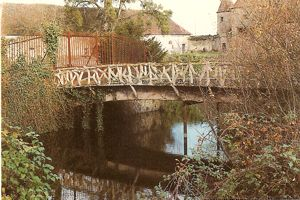
\includegraphics[max width=\textwidth]{Monier_bridge_Chazelet.jpg}
	\end{center}
	\fonte{\citeonline{chazelet}.}
\end{figure}

Monier vendeu suas patentes de concreto armado em 1884 para duas empresas alemãs, que posteriormente foram vendidas para o engenheiro alemão Gustav Wayss em 1886, da empresa Wayss \& Freytag. Wayss passou a investir em pesquisa e um de seus funcionários, Mörsch, foi quem aprimorou e estabeleceu bases científicas para o concreto armado, escrevendo o livro intitulado ``Der Betoneisenbau: Seine theorie und Anwendung'' (Construções de Concreto e Aço: Sua teoria e aplicação).

O primeiro edifício em concreto armado feito no Brasil foi construída pela Wayss \& Freytag em 1907, na rua São Bento, em São Paulo - SP. Possuía apenas três pavimentos, mas já era um marco para a época.

Os primeiros estudos acerca de concreto protendido começaram na década de 20, possibilitando a construção de estruturas mais esbeltas, leves e capazes de vencer vãos maiores do que o concreto armado é capaz de suportar.

A popularidade do concreto deve-se, principalmente, às seguintes características:

\begin{alineas}[label=\textbullet]
  \item Disponibilidade de matéria prima: 89\% da crosta terrestre é formada por 90\% dos materiais que compõem o concreto;
  \item Versatilidade na modelagem: em seu estado fresco é um material plástico, se adequando a qualquer forma desejada;
  \item Sólido: depois da cura, se torna um material, praticamente homogêneo, solidarizado entre si;
  \item Durável: tomadas as devidas precauções, o concreto é capaz de resistir aos efeitos do tempo e do ambiente;
  \item Custo: por conta da disponibilidade de matéria prima e bom desempenho, é um material extremamente competitivo na cadeia de materiais de construção civil;
  \item Sustentabilidade: quando bem executadas, as estruturas de concreto são muito duráveis, é um material facilmente encontrado e de produção regional, utiliza rejeitos industriais como adição e seu entulho é totalmente reciclável.
\end{alineas}

Apesar disso, o concreto ainda possui algumas desvantagens, como baixa resistência à tração, elevado peso próprio, acentuada variação volumétrica e dificuldade na moldagem de peças de grande volume, devido ao calor gerado na hidratação. Cada um destes problemas tem uma solução específica, a ser determinada pelo projetista.

\section{Tecnologias de construções de concreto}

O concreto, quando não associado a nenhum outro material, é denominado concreto simples. O concreto simples é incapaz de suportar seu próprio peso, já que o material possui uma capacidade de resistência à tração muita baixa (cerca de 10\% de sua resistência a compressão), de modo que, para se construir edificações, é necessário associá-lo a outras materiais, sendo o método mais comum e difundido, a associações do concreto com o aço. As seguintes seções apresentam mais detalhes desta associação e da industrialização do método.

\subsection{Concreto armado}

Concreto armado é um material de construção civil que consiste na combinação do concreto simples com uma armadura de aço. O concreto resiste aos esforços de compressão aos quais a estrutura será solicitada e fornece ao aço um ambiente alcalino que o protege dos efeitos corrosivos do ambiente, dado uma espessura mínima de cobrimento de concreto sobre a armadura. Por sua vez, o aço (após a fissuração inicial do concreto) resiste aos esforços de tração aos quais a estrutura é solicitada, o que ocorre devido à aderência de uma material ao outro. Outro fator determinante para a escolha destes dois materiais são os seus respectivos valores do coeficiente de dilatação térmica, próximos entre si, o que garante que as deformações térmicas sofridas pelo aço são praticamente iguais à do concreto.

A armadura de aço contida nos elementos estruturais de concreto armado é chamada de armadura passiva, pois ele só começa a ser solicitada quando algum carregamento é adicionado à estrutura. O concreto, por sua vez, incapaz de suportar os esforços de tração, fissura e, por conta da aderência da interface concreto-aço, os esforços são transmitidos à armadura, a qual passa a resistir aos esforços de tração.

\subsection{Concreto protendido}

Concreto protendido é um material de construção civil que consiste na combinação de concreto simples com cabos de aço protendido, isto é, pré ou pós tensionado. Estes cabos comprimem o concreto, o qual não fissura na iminência de um carregamento que gere esforços de tração, já que os cabos protendidos recebem estes carregamentos de maneira ativa, diferentemente do concreto armado, onde a armadura age de maneira passiva. Desse modo, a protensão diminui ou anula as solicitações de tração no concreto e ainda melhora a resistência ao cisalhamento e à torção da peça estrutural.


\subsection{Concreto pré-moldado}

O concreto pré-moldado é uma peça estrutural ou decorativo produzida de maneira industrializada, os quais, posteriormente, são transportados para montagem final. O seu processo de produção visa diminuir o tempo de construção e mobilização de trabalhadores no canteiro de obras.
 
\section{Concretos especiais}

O século XX foi marcado pela busca da otimização dos processos de produção e de projeto de estrutura de concreto, mas ao que tudo indica, o século XXI será marcado pela busca otimização do concreto em si, afim de torná-lo um material ainda mais barato, versátil e capaz de competir ainda mais com o aço na construção civil. Nesta seção, apresenta-se as últimas tecnologias disponíveis para o uso de concreto na construção civil:

\begin{alineas} %[label=\textbullet]
  \item \textbf{Concreto de alto desempenho (CAD):} trata-se de uma classe de concreto com resistências superiores ao concreto convencional, de 40 MPa a 100 MPa;
  
  \item \textbf{Concreto de ultra alto desempenho (CUAD):} trata-se de uma nova classe de concretos especiais. Este trabalho expõe este material em detalhes no \autoref{chap:CUAD};
  
  \item \textbf{Concreto com aditivos especiais:} aditivos são materiais que, adicionados ao concreto, são capazes de mudar seu comportamento fisíco e/ou químico, de acordo com a necessidade da construção. Abaixo, lista-se alguns exemplos de aditivos disponíveis no mercado e suas características:
    \begin{incisos}
      \item \textbf{Acelerador de pega:} para uma moldagem rápida e consequente breve desforma;
      
      \item \textbf{Adição de minerais pozolânicos:} este aditivo é obtido em regiões de atividade vulcânica ou feito artificialmente em fornos industriais. Dos aditivos desta categoria, o principal é a cinza volante, utilizada para retardar a hidratação do concreto e diminuir sua reação álcali-agregado, retartando o ganho inicial de resistência mecânica e diminuindo a quantidade de calor liberado durante a hidratação. Com isso, a incidência de fissuras em peças volumosas de concreto é inibida;
      
      \item \textbf{Aditivos diminuidores ou compensadores de retração:} esses aditivos visam resolver o mesmo problema: retração do concreto e empenamento das placas de piso;
      
      \item \textbf{Aditivos tensoativos:} ajuda a incorporar ar no concreto, diminuindo a tensão superficial que a água causa. Assim reduz a segregação e exsudação, mas diminuindo a resistência mecânica;
      
      \item \textbf{Plastificantes/redutores de água:} aumenta a trabalhabilidade do concreto sem a necessidade de se adicionar mais água. A adição desse material é de 0,2 a 0,7\% da massa de cimento, e pode representar cerca de 20\% na redução de água na pasta;
      
      \item \textbf{Rebarbas metálicas e carbono:} visa transformar o concreto em um material condutor de eletricidade, utilizando a própria peça estrutural para aquecer o ambiente ou derreter gelo e neve em áreas externas;
      
	  \item \textbf{Retardador de pega:} assim como o nome já diz, aumenta o tempo disponível para se trabalhar com o concreto. Muito utilizado durante concretagens demoradas e locais de clima quente. Pode retardar o início da pega em até 8 horas;
    \end{incisos}
    
    \item \textbf{Concreto com fibras:} a adicão de fibras ao concreto tem como finalidade redistribuir de maneira mais uniforme os esforços a qual a peça estrutural é solicitada, predominantemente na seção de tração, pois aumenta seu módulo de elasticidade sem diminuir sua resistência mecânica. Sua aplicação é mais comum em rodovias, pisos industriais e pistas de aeroportos. As fibras podem ser de aço, polipropileno, vidro, carbono, poliéster e nylon, entre outras;
    
    \item \textbf{Concreto leve estutural:} o concreto leve estrutural substitui o agregado comum por agregados leves (pedra pomes, escória vulcânica, argila expandida e escória expandida), fazendo com que sua massa específica seja 20\% menor que a do concreto convencional. Por conta de empregar o uso de agregados porosos, estruturas feitas com concreto leve estrutural sofrem de deformações mais acentuadas, já que seu módulo de elasticidade varia de 50\% a 80\% do concreto convencional. O agregado leve também tende a se acumular na superfície durante a concretagem, além de absorver água, fator que deve ser levado em consideração na hora de se determinar o traço do concreto. O acúmulo do agregado na superfície pode ser controlado com os agregados miúdos;
    
    \item \textbf{Concreto arquitetônico e decorativo:} 
    o concreto sem fim estrutural ou também conhecido como arquitetônico, tem mesmo desempenho de um concreto convencional. Pigmentos inertes podem ser adicionados para dar coloração ao concreto;
    
   
    \item \textbf{Concreto para blindagem de radiação:} utiliza-se agregados pesados, como hematita, de acordo com a intensidade da radiação a qual estará exposto;
    
    \item \textbf{Concreto fotocalítico:} com a incorporação de dióxidos de titânio ou silício em sua composição ou em sua superfície, é possível transformar gases nocivos, como óxido de nitrogênio em nitratos essenciais para o desenvolvimento das plantas, através da fotocálise;
    
    \item \textbf{Concreto autocicatrizante:} incorpora-se bactérias capazes metabolizar os componentes necessários para fechar pequenas fissuras no concreto. As bactérias ficam inertes e só entram em ação em contato com água. Para isso, são adicionados retentores de água no concreto, os quais se rompem no aparecimento de uma fissura;
    
    \item \textbf{Concreto translúcido:} utiliza como aditivo fibras óticas poliméricas. Tem bastante potencial para iluminar ambientes e provocar a diminuição do consumo de energia elétrica.
    
\end{alineas}

\chapter{Concreto de ultra alto desempenho ({CUAD})}
\label{chap:CUAD}

O concreto de ultra alto desempenho agrega o que existe de mais moderno nos setores de pesquisa e desenvolvimento de concreto. Pode-se dizer que CUAD é uma classe de concretos com resistência e durabilidade superiores ao CAD (concreto de alto desempenho), o qual já é utilizado de maneira mais corriqueira em grandes obras.

Apresenta-se um breve histórico do desenvolvimento do CUAD, as principais linhas de pesquisa em estudo, características e obtenção do material, aspectos ambientais e de custo-benefício, além de sua aplicação no Brasil e no mundo.

\section{Breve histórico do concreto de ultra alto desempenho}

Sempre buscou-se o desenvolvimento de um concreto cada vez mais resistente e mais fácil de se trabalhar. Inicialmente, essas duas características se rivalizam, pois, a relação água/aglomerante influencia tanto a trabalhabilidade do concreto como sua resistência. Uma maior quantidade de água melhora a trabalhabilidade do concreto, mas aumenta sua porosidade e diminui sua resistência e durabilidade. Por outro lado, se a quantidade de água for muito pequena, o concreto terá uma baixa trabalhabilidade, dificultando o trabalho dos operários.

\nomenclature[S]{MPa}{Megapascal}

\apudonline{Fuller}{Carneiro} demonstrou empiricamente que, dada uma porcentagem de cimento em determinado volume de concreto, havia uma distribuição ótima de tamanhos do grão de agregado a qual aumentava a sua resistência mecânica e atingia uma melhor trabalhabilidade, concluindo que a distribuição granulométrica dos agregados influencia diretamente na compacidade do concreto, que por sua vez, influencia em sua resistência mecânica (quanto maior a compacidade, maior a resistência mecânica).

Na década de 1930, Eugène Freyssinet demonstrou que, a aplicação de pressão no concreto fresco ainda na forma, aumentava sua resistência mecânica. O processo expulsa o ar preso no concreto durante a mistura e expulsa o excesso de água, diminuindo a relação água/aglomerante. Nos anos 60, apenas com a aplicação deste princípio (com elevada pressão) e cura térmica, foram alcançados valores de resistência de 650 MPa \apud[p.~8]{Richard_e_Cheyrezi}{Vanderlei}.

%.

%O desenvolvimento de superplastificantes (para diminuir a relação água/aglomerante), aditivos, pigmentos e fibras para concreto, assim como o uso de técnicas inovadoras de execução podem, teoricamente, fazer com que o concreto possa atender qualquer solicitação de projeto, tendo como limitante apenas o custo da execução.

Segundo \citeonline[p.~5]{Resplendino}, as primeiras pesquisas sobre a tecnologia do CUAD começaram nos anos 70, com o pesquisador Bache, na Dinamarca. Suas pesquisas resultaram no desenvolvimento do CRC (\textit{Compact Reinforced Composite}, em português, CCR - Compósito Compacto Reforçado). Na Europa o CRC é muito utilizado na composição de pré-fabricados, porém eles são reforçados por armaduras convencionais, calculadas de modo que não se leva em consideração a participação mecânica das fibras \cite[p.~6]{Resplendino}. Segundo \citeonline{Aitcin}, nos anos 1972-1973, Brunanauer desenvolveu um compósito capaz de resistir uma solicitação de compressão de até 200 MPa, o qual foi patenteado sob o nome de DSP (\textit{Densified with Small Particles} ou DPP - Densificado de Partículas Pequenas), baseado no conceito de compactação da matriz granulométrica. Posteriormente, Birchall et al. desenvolveram um concreto de ultra alto desempenho a partir de uma abordagem diferenciada, denominado de MDF (\textit{Macro Deffect Free} ou LMD - Livre de Macros Defeitos) \cite{Aitcin}. O MDF incorpora o conceito de pasta polimérica, garantindo uma resistência a tração na flexão de 150 MPa ou mais, especialmente quando se utiliza cimento aluminoso. Desse modo, as principais linhas de pesquisa da atualidade se dividem em dois ramos: uma pesquisa a utilização de materiais finíssimos na composição do concreto e a outra, a utilização de pastas poliméricas na composição do concreto \cite[p.~8]{Vanderlei} e duas abordagens de pesquisa: uma baseada em uma análise empírica, a partir da construção de modelos em escala e estudo de comportamento e carregamento da estrutura, como a utilizada pela \textit{Association Française de Genie Civil} (AFGC) e outra que deriva os efeitos macroscópicos de fenômenos em escala miscroscópica e nanoscópica, conhecido como micromecânica. Trata-se de um processo altamente analítico, demandando muito mais tempo para que se possa entender, mas que, quando formas as suas bases, permite uma fácil modificação para incluir efeitos mecânicos provenientes da temperatura (termomicromecânica), porosidade (poromicromecânica) e química (quimiomicromecânica) \cite{Davila}. 


\nomenclature[A]{AFGC}{\textit{Association Française de Genie Civil}}
\nomenclature[A]{JSCE}{\textit{Japan Society of Civil Engineers}}
\nomenclature[A]{CRC}{\textit{Compact Reinforced Composite}}
\nomenclature[A]{CCR}{Compósito Compacto Reforçado}
\nomenclature[A]{DSP}{\textit{Densified with Small Particles}}
\nomenclature[A]{DPP}{Densificado de Partículas Pequenas}
\nomenclature[A]{MDF}{\textit{Macro Deffect Free}}
\nomenclature[A]{LMD}{Livre de Macros Defeitos}

Diversos compósitos de base cimentícia possuem alta resistência e superior durabilidade, os quais pode-se dizer que se enquadram na categoria de concreto de ultra alto desempenho (CUAD). Além das variedades citadas acima, por \citeonline{Russel_e_Graybeal} e outras de desenvolvimento mais recente, tem-se:

\begin{alineas}[label=\textbullet]
  %\item CRC - \textit{compact reinforced composite} (CCR - compósito compacto reforçado);
  \item FRHPC - fiber-reinforced high-performance concrete (CADRF - concreto de alto desempenho reforçado com fibras);
  \item HPFRCC - high-performance fiber reinforced cement composite (CCADRF - compósito cimentício de alto desempenho reforçado com fibras);
  \item MSFRC - multi-scale fiber-reinforced concrete (CMSRF - concreto multiescalável reforçado com fibras);
  \item RPC - reactive powder concrete (CPR - concreto de pós reativos);
  \item SFCBC - steel fibrous cement-based composite (CCFA - compósito cimentício fibroso de aço)
  \item UHPFRCC - ultra-high performance fiber-reinforced cementitious composite (CCUADRF - compósito cimentício de ultra alto desempenho reforçado com fibras);
  \item UHPFRC - ultra-high performance fiber-reinforced concrete (CUADRF - concreto de ultra alto desempenho reforçado com fibras);
  \item UHSC - ultra-high strength concrete (CUAR - concreto de ultra alta resistência);
  \item Compósito cimentício de ultra alta resistência;
  \item Compósito cimentício de ultra resistência reforçado com fibras.
  \item UHPGC - ultra-high performance glass concrete (CVUAD - concreto de vidro de ultra alto desempenho) \cite{Soliman};
  \item GUHPC - geopolymer composite ultra high performance concrete (CGCUAD - compósito geopolimérico de concreto de ultra alto desempenho)\cite{Gong}.
\end{alineas}

\nomenclature[A]{FRHPC}{\textit{Fiber-reinforced high-performance concrete}}
\nomenclature[A]{CADRF}{Concreto de alto desempenho reforçado com fibras}
\nomenclature[A]{HPFRCC}{\textit{High-performance fiber reinforced cement composite}}
\nomenclature[A]{CCADRF}{Compósito cimentício de alto desempenho reforçado com fibras}
\nomenclature[A]{MSFRC}{\textit{Multi-scale fiber-reinforced concrete}}
\nomenclature[A]{CMSRF}{Concreto multiescalável reforçado com fibras}
\nomenclature[A]{RPC}{\textit{Reactive powder concrete}}
\nomenclature[A]{CPR}{Concreto de pós reativos}
\nomenclature[A]{SFCBC}{\textit{Steel fibrous cement-based composite}}
\nomenclature[A]{CCFA}{Compósito cimentício fibroso de aço}
\nomenclature[A]{UHPFRCC}{\textit{Ultra-high performance fiber-reinforced cementitious composite}}
\nomenclature[A]{CCUADRF}{Compósito cimentício de ultra alto desempenho reforçado com fibras}
\nomenclature[A]{UHPFRC}{\textit{Ultra-high performance fiber-reinforced concrete}}
\nomenclature[A]{CUADRF}{Concreto de ultra alto desempenho reforçado com fibras}
\nomenclature[A]{UHSC}{\textit{Ultra-high strength concrete}}
\nomenclature[A]{CUAR}{Concreto de ultra alta resistência}
\nomenclature[A]{UHPGC}{\textit{Ultra-high performance glass concrete}}
\nomenclature[A]{CVUAD}{Concreto de vidro de ultra alto desempenho}
\nomenclature[A]{GUHPC}{\textit{Geopolymer composite ultra high performance concrete}}
\nomenclature[A]{CGCUAD}{Compósito geopolimérico de concreto de ultra alto desempenho}

\nomenclature[S]{a/c}{Relação água/cimento}
\nomenclature[S]{kg/MNm}{Quilograma por meganewton metro}
\nomenclature[S]{$\text{kg/m}^3$}{Quilograma por metro cúbico}
\nomenclature[S]{GPa}{Gigapascal}
\nomenclature[S]{mm}{Milímetro}

Historicamente, pode-se observar uma relação muito próxima entre a tecnologia existente e os materiais disponíveis para construção e a arquitetura das construções. Ainda que o CUAD seja chamado de “concreto”, trata-se de um material completamente novo, exigindo um novo olhar sobre como ele deve ser utilizado nas construções. Não faz nenhum sentido utilizar um material com desempenho tão elevado do mesmo modo que utilizamos o concreto convencional. Outro ponto a se notar é que a popularidade de um material é diretamente afetada pelo seu custo. Assim como a produção de aço foi revolucionada pela Bessemer and Open Hearth Steel na década de 1850, produzindo aço em grande escala a preços acessíveis, fazendo com que as pessoas passassem a utilizá-lo nas construções, o CUAD também precisa passar por um processo similar, de modo que essa tecnologia possa ser trazida a aplicações populares \cite[p.~9]{Tang}.

Neste trabalho, utiliza-se a definição genérica concreto de ultra alto desempenho (CUAD), salvo quando houver necessidade de especificar uma variedade.

\section{Definição e características do CUAD}

%A \citeonline[p.~7, tradução nossa]{AFGC} define CUAD da seguinte maneira:
%
%\begin{citacao}
%"Concreto de ultra alto desempenho reforçado com fibras"~se refere a materiais com matriz cimentícia e características de resistência à compressão que excedem 150 MPa, possivelmente chegando a 250 MPa, e contendo fibras de aço para atingir comportamento dúctil sob tensão e, se possível, dispensar o uso de armadura passiva (não protendida). Também pode conter polímeros.
%\end{citacao}
%
%\nomenclature{CAD}{Concreto de alto desempenho}
%
%A \citeonline[p.~7, tradução nossa]{AFGC} ainda destaca que o CUAD se diferencia do concreto de alto de desempenho (CAD) conforme as seguintes características:
%
%\begin{citacao}
%\textbullet~~O CUAD possui uma resistência a compressão maior que 150 MPa, enquanto o CAD varia entre 35 MPa e 100 MPa; \\ 
%\textbullet~~O CUAD usa fibras, assegurando que o material não seja quebradiço e modificando os requisitos convencionais para reforço com armadura passiva/ativa. O CAD normalmente não possui fibras; \\
%\textbullet~~O CUAD usa muito aglomerante de modo a reduzir drasticamente o uso de água e possui seleção especial de agregados.
%\end{citacao}

O CUAD é um compósito de matriz cimentícia, composto de aglomerante, agregado miúdo, fibras (metálicas, naturais ou sintéticas) que, ao contrário do concreto convencional, é capaz de suportar grandes cargas de compressão (normalmente de 150 MPa a 250 MPa, mas podendo chegar a 800 MPa em condições especiais) e possui comportamento dúctil, devido às fibras adicionadas ao compósito. Caracteriza-se também pela alta quantidade de aglomerante, baixa relação água/aglomerante (o que garante um material de alta densidade) baixa porosidade, microestrutura extremamente cerrada e cura térmica a elevadas temperaturas, em atmosfera saturada de vapor \cite{AFGC}. Desse modo, este material possui uma elevada durabilidade, possui baixa permeabilidade para cloridos (composto químico extremamente corrosivo para concreto), grande resistência a congelamento-descongelamento e grande resistência a ataques de ácidos e sulfatos \cite[p.~7-11]{Resplendino}. É importante notar que a cura térmica também melhora as propriedades do concreto convencional, pois sua aplicação acelera as reações de hidratação do cimento. A exposição precoce do concreto com altas temperaturas reduz o período de latência e define a estrutura da pasta de cimento mais cedo, a qual enrijece mais rápido e tem um tempo de início de pega mais curto \apud[p.~4]{Neville}{Palma}. \apudonline[p.~4]{Camarini}{Palma} afirma que a cura térmica é considerada a cura mais eficiente, principalmente quando se trata de concreto pré-moldado, ao proporcionar o melhor aproveitamento dos equipamentos necessários para a moldagem do concreto.

Segundo \apudonline[p.~4]{Camarini}{Palma}, a cura térmica em atmosfera saturada de vapor é feita de duas maneiras:

\begin{alineas}[label=\textbullet]
  \item com pressão de aproximadamente 1 MPa e temperaturas entre 150\textsuperscript{\degree}C e 205\textsuperscript{\degree}C (cura em autoclave);
  \item à pressão atmosférica, com temperaturas menores que 100\textsuperscript{\degree}C.
\end{alineas}

Como o CUAD exige um rígido controle de qualidade para atingir altas resistências, é recomendável que sua produção seja industrializada, assim como já se faz na indústria de concreto pré-moldado com o concreto convencional ou o concreto de alto desempenho.

Segundo o \citeonline{CBI}, pode-se dizer, resumidamente, que o CUAD é composto de: %(\autoref{componentes}): 

\begin{alineas}[label=\textbullet]
  \item cimento;
  \item fíler (quartzo, pó de cinza, escória);
  \item areia;
  \item água;
  \item superplastificante;
  \item fibras (metálicas ou poliméricas).
\end{alineas}

E caracteriza-se por:

\begin{alineas}[label=\textbullet]
  \item baixa relação água/aglomerante;
  \item alta dosagem de superplastificante;
  \item auto adensamento;
  \item microestrutura densa;% (\autoref{empacotamento});
  \item cura térmica.
\end{alineas}

É importante notar que o cimento não é o único aglomerante que pode ser utilizado para fazer o CUAD. Pesquisas recentes mostram que alternativas como geopolímeros e pó de vidro podem substituí-lo na mistura dos materiais, os quais podem ser até mais sustentáveis e baratos que o cimento \cite{Goldoni} \cite{Soliman}.

%\begin{figure}[htb]
%	\caption{\label{porosidade}Porosidade do CUAD em relação ao concreto convencional.}
%	\begin{center}
%	    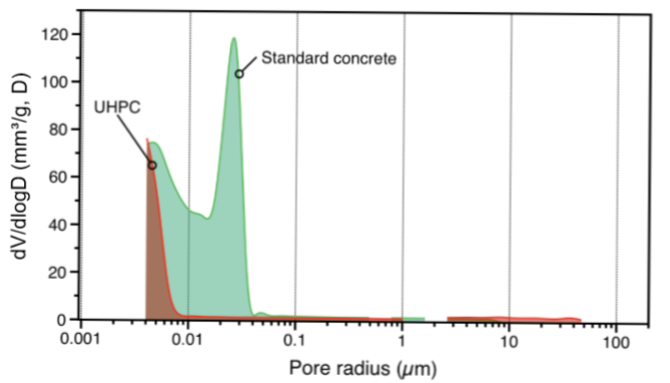
\includegraphics[max width=\textwidth]{porosidade.png}
%	\end{center}
%	\fonte{\citeonline{CBI}}
%\end{figure}

%\begin{figure}[htb]
%	\caption{\label{componentes}Materiais que compõem o CUAD.}
%	\begin{center}
%	    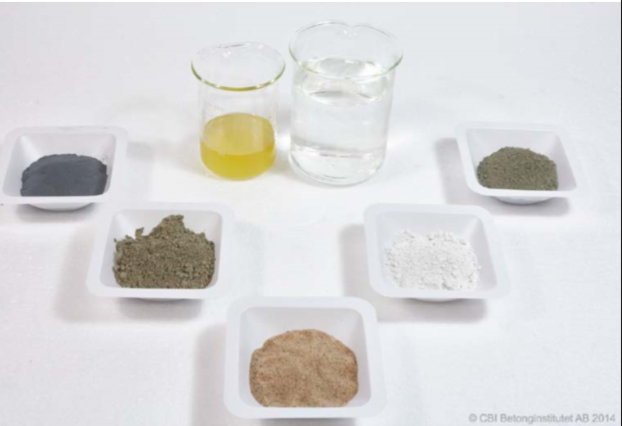
\includegraphics[max width=\textwidth]{componentes.png}
%	\end{center}
%	\fonte{\citeonline{CBI}}
%\end{figure}
%
%\begin{figure}[htb]
%	\caption{\label{empacotamento}Comparação entre a microestrutura dos agregados no concreto padrão x CUAD.}
%	\begin{center}
%	    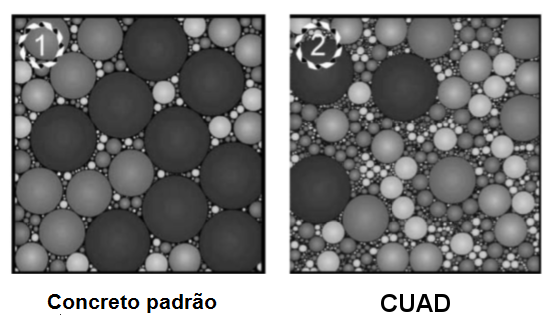
\includegraphics[max width=\textwidth]{empacotamento.png}
%	\end{center}
%	\fonte{\citeonline{CBI}}
%\end{figure}

Tipicamente, o CUAD resiste a solicitações de compressão de 200 MPa e à ruptura dúctil de 10 a 15 MPa. Ainda é capaz de suportar deformação e carregamentos de flexão e tensão mesmo após a fissuração inicial do concreto, devido à dissipação de energia do material ser maior devido à sua microestrutura densa \cite[p.~1]{Gunes}. Sua razão de massa para resistência é de aproximadamente 15 kg/MNm, em contraste com a razão de 40 a 120 kg/MNm do concreto convencional \cite[p.~461]{Stengel}. \apudonline{Tuan}{Gu} comparou a composição e as propriedades do concreto convencional, CAD e CUAD.  Os detalhes são mostrados na \autoref{comparacao}.

\begin{table}[htb]
\IBGEtab{%
  \caption{Comparação da composição do concreto convencional, CAD e CUAD}
  \label{comparacao}
}{%
  \begin{tabulary}{\linewidth}{CCCC}
  \toprule
                                                & Concreto convencional  & CAD & CUAD \\
  \midrule \midrule
   Cimento (kg/m\textsuperscript{3})            & <400                   & 400       & 600-1000 \\ \midrule 
   Agregado graúdo (kg/m\textsuperscript{3})    & $\approx$ 1000         & 900       & - \\ \midrule 
   Areia (kg/m\textsuperscript{3})              & $\approx$ 700          & 600       & 1000-1200 \\ \midrule 
   Fumo de sílica (kg/m\textsuperscript{3})     & -                      & 40        & 50-300 \\ \midrule 
   Armadura/fibras (kg/m\textsuperscript{3})    & Projetado              & Projetado & 40-250 \\ \midrule 
   Superplastificante (kg/m\textsuperscript{3}) & -                      & 5         & 10-70 \\ \midrule 
   Água (kg/m\textsuperscript{3})               & > 200                  & 100-150   & 110-260 \\ \midrule    
   Tamanho máximo do agregado (mm)              & 19,0-25,5              & 9,5-12,5  & 0,15-0,6 \\ \midrule    
   Relação água/cimento (a/c)                   & 0,40-0,70              & 0,24-0,38 & 0,14-0,27 \\
  \bottomrule
\end{tabulary}%
}{%
  \fonte{\apudonline[p.~589]{Tuan}{Gu}.}%
  %\nota{Recomenda-se o uso de água de amassamento de baixa temperatura, pré cura térmica de 2 dias e cura térmica de 24 horas a uma temperatura de 80\textsuperscript{\degree} C.}
  %\nota[Anotações]{Uma anotação adicional, que pode ser seguida de várias outras.}
  }
\end{table}

\subsection{Módulo de elasticidade}

O módulo de elasticidade do CUAD varia de acordo com o traço utilizado, característica dos agregados e o regime de cura, ficando entre 40 a 70 GPa. Seu módulo de elasticidade é maior que o apresentado pelo concreto convencional e pelo CAD, devido à sua microestruturas densa e adição de fibras \cite[p.~591]{Gu}.

\subsection{Retração}

O CUAD apresenta três tipos de retração: química, autógena e de secagem, afetadas principalmente pela relação água/aglomerante. Das três, o tipo de retração mais predominante, assim como observado no concreto de alto desempenho (CAD) \cite[p.~408]{Neville2}, é a autógena, por conta da baixa relação água/aglomerante, existindo um alto risco de micro-fissuração na idade jovem do concreto caso ele se encontre restringido. De modo a compensar a retração autógena, é possível utilizar um aditivo expansivo ou um aditivo de redução da retração, cuidadosamente dosados para a mistura. Outra solução é aplicar cura interna, descrita pelo ACI (\textit{American Concrete Institute}, em português, Instituto Americano de Concreto) como ``fornecimento água através de uma mistura de cimento recém-colocada usando reservatórios, através de agregados leves ligeiramente pré-molhados, que descartam facilmente a água conforme necessário para a hidratação ou para substituir a umidade perdida por evaporação ou auto-dessecação''. Como não é possível utilizar agregados leves no CUAD, pesquisadores investigam a possibilidade de se utilizar polímeros superabsorventes como agentes de cura interna \cite[p.~592]{Gu}.

\nomenclature[A]{ACI}{\textit{American Concrete Institute}}

\subsection{Deformação}

O coeficiente de deformação do CUAD varia de 0,3 a 0,85, e a deformação específica de 5 a 47 {\textmu}m/m/MPa, sendo que a deformação do concreto pode ser expressada por um coeficiente de deformação (tensão de deformação/tensão inicial) ou deformação específica (tensão de deformação/força aplicada). Para efeito de comparação, a deformação específica do concreto convencional varia de 35 a 140 {\textmu}m/m/MPa \cite[p.~592]{Gu}.

\nomenclature[S]{{\textmu}m/m/MPa}{Micrometro por metro por megapascal}

\subsection{Propriedades térmicas}

As recomendações da \citeonline{AFGC} possuem uma tabela com o coeficiente de dilatação térmica para diferentes misturas de CUAD. Caso a mistura não esteja disponível na tabela, o valor geral a ser utilizado deve ser de 11 {\textmu}m/m/\textsuperscript{\degree}C \cite[p.~592]{Gu}.

\nomenclature[S]{{\textmu}m/m/\textsuperscript{\degree}C}{Micrometro por metro por grau Celsius}
\nomenclature[S]{m/s}{Metro por segundo}
\nomenclature[S]{kN/$\text{m}^2$}{Quilonewton por metro quadrado}
\nomenclature[S]{m/$\text{s}^2$}{Metro por segundo ao quadrado}
\nomenclature[S]{fck}{Resistência característica do concreto}

\subsection{Resistência ao fogo}
\label{fogo}
Apesar do CUAD não ser um material inflamável, assim como todo concreto, sua microestrutura cerrada o torna mais suscetível ao lascamento (\textit{spalling}) explosivo durante o aquecimento. Este fenômeno ocorre por conta de pressão nos poros devido a esforços térmicos e desidratação dos hidratos. Fibras de prolipropileno é uma das soluções adotadas para evitar este comportamento \cite[p.~592]{Gu}.

\subsection{Comportamento na fadiga}

Como o CUAD é um material recente, existem poucos estudos sobre seu comportamento na fadiga, os quais mostram que ele possui uma excelente resistência à fadiga, ao contrário do que ocorre com outros materiais de alta resistência \cite[p.~592]{Gu}.

\subsection{Resistência à impacto}

A resistência à impacto do CUAD é  muito superior à do concreto convencional ou mesmo do concreto com fibras, por conta do forte vínculo entre as fibras e a matriz cimentícia, de modo que o CUAD é um ótimo material para aplicações militares e construção de estruturas que precisem resistir a explosões ou penetrações \cite[p.~592]{Gu}.

%\subsection{Durabilidade}



\section{CUAD do tipo CPR (concreto de pós reativos)}

Existe muitas variedades de CUAD disponíveis no mercado, mas segundo \citeonline[p.~1312-1313]{Tutikian}, o CPR (concreto de pós reativos) é o CUAD que possui a maior dedicação dos centros de pesquisa. É sobre essa variedade de CUAD que este trabalho se concentra, já que essa é a variedade disponível no Brasil, comercializada pela LafageHolcim sob o nome de Ductal\textsuperscript{\textregistered}.

\citeonline[p.~1313]{Tutikian} afirma que a “ideia básica desse novo tipo de concreto foi eliminar os inconvenientes dos agregados graúdos [...] como as possíveis oclusões ou vazios internos, eliminação da zona de transição e aumento da superfície do esqueleto granular”. O seguinte excerto explica melhor suas características:

\begin{citacao}
Pelo efeito da maior superfície específica, a distribuição das cargas incidentes sobre os grãos é mais homogênea, diminuindo a concentração de tensões em eventual falha da microestrutura, assim, aumentando a resistência última do material. Sabe-se que, quanto menor a dimensão dos grãos, maior é a superfície específica, maior a reatividade química e ligações secundárias pelas forças de van der Waals (ligações de superfície) e mais elevada é a homogeneidade do material. Dessa forma, os grãos de agregados finos não ficam em contato um com os outros, evitando as tensões de contato e possíveis falhas nesses locais \cite[p.~1312]{Tutikian}.
\end{citacao}

\citeonline{Aitcin} resume o conceito do CPR em três princípios básicos:

\begin{citacao}
\textbullet~Aumento da homogeneidade do material pela eliminação das partículas grossas, limitação da areia para prevenir que entrem em contato entre si na pasta endurecida, melhoria nas propriedades mecânicas da pasta de cimento hidratada e eliminação da zona de transição nas interfaces pasta/agregados;\\
\textbullet~Aumento da compacidade pela otimização das dimensões dos grãos dos pós da mistura e, quando possível, pela compressão exercida durante o endurecimento;\\
\textbullet~Refinamento da microestrutura da pasta hidratada por tratamento de calor.
\end{citacao}

\citeonline{Vanderlei_e_Giongo} definem os princípios para obtenção do CPR da seguinte forma:

\begin{alineas}[label=\textbullet]
  \item eliminação dos agregados graúdos para aumentar a homegeinidade;
  \item compressão do material durante o preparo (antes e durante a concretagem, diminuindo a incorporação de ar, removendo o excesso de água e compensando a retração química) e/ou otimização da distribuição granulométrica dos agregados miúdos de modo a aumentar a densidade do material;
  \item cura térmica para fortalecer a microestrutura;
  \item uso de fibras ou tubos metálicos preenchidos com CPR para aumentar a ductilidade;
\end{alineas}

Do ponto de vista da granulometria dos agregados que compõem o CPR (diâmetro máximo de 0,2 mm), ele deveria ser considerado uma argamassa, mas convencionou-se chamá-lo de concreto devido ao desempenho exibido pelo material \cite[p.~1313]{Tutikian}.

\citeonline{Vanderlei_e_Giongo} demonstram que a indústria brasileira já produz os materiais necessários para obtenção do CPR. Assim como \citeonline{Tutikian},  recomendam o uso de cimento CPV ARI. A dosagem de CPR proposta por \citeonline{Vanderlei_e_Giongo} é mostrada na \autoref{dosagem-cpr}.

\begin{table}[htb]
\IBGEtab{%
  \caption{Dosagem para concretos de pós reativos.}
  \label{dosagem-cpr}
}{%
  \begin{tabulary}{\linewidth}{CCC}
  \toprule
   Material                 & Relação (em massa) & Consumo $\text{kg/m}^3$ \\
  \midrule \midrule
   Cimento                  & 1                  & 874 \\ \midrule 
   Areia                    & 1,101              & 962 \\ \midrule 
   Pó de quartzo            & 0,235              & 205 \\ \midrule 
   Sílica ativa             & 0,246              & 214 \\ \midrule 
   Superplastificante (3\%) & 0,030              & 26  \\ \midrule 
   Água (a/c = 0,18)        & 0,180              & 157 \\
  \bottomrule
\end{tabulary}%
}{%
  \fonte{\citeonline[p.~119]{Vanderlei_e_Giongo}.}%
  \nota{Recomenda-se o uso de água de amassamento de baixa temperatura, pré cura térmica de 2 dias e cura térmica de 24 horas a uma temperatura de 80\textsuperscript{\degree}C.}
  %\nota[Anotações]{Uma anotação adicional, que pode ser seguida de várias outras.}
  }
\end{table}

É importante notar que a dosagem \citeonline{Vanderlei_e_Giongo} é condizente com a realidade brasileira, portanto difere da utilizada por outros estudos internacionais, em virtude da diferença geográfica.

A adição de fibras é o fator determinante na resistência à tração na flexão do CPR, que passam a influenciar este fator em uma taxa a partir de 1\% \cite[p.~138]{Vanderlei_e_Giongo}. A \autoref{taxa-fibras} mostra a influência da taxa de fibras na resistência à tração na flexão do CPR observada nos corpos de prova moldados pelos autores. Este fenômeno ocorre pois as fibras distribuem melhor os esforços na matriz do concreto, porém, como sua distribuição não pode ser controlada, normalmente é preciso lançar mãos de outros métodos para garantir a resistência do concreto a esforços de tração na flexão.

\begin{figure}[htb]
	\caption{\label{taxa-fibras}Influência da taxa de fibras na resistência à tração na flexão do CPR.}
	\begin{center}
	    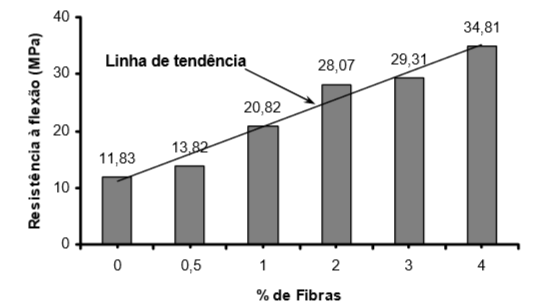
\includegraphics[max width=\textwidth]{taxa-fibras.png}
	\end{center}
	\fonte{\citeonline[p.~138]{Vanderlei_e_Giongo}}
\end{figure}

Ainda não existe uma consolidação de como deve ser feito o estudo de dosagem do CPR. \citeonline[p.~42]{Vanderlei} e \citeonline[p.~32]{Christ} informam que métodos matemáticos de empacotamento de partículas têm bastante êxito nessa tarefa.

\section{Sustentabilidade e custo-benefício}

Devido a demandas sociais e ambientais, a indústria da construção passou a incluir sustentabilidade no cálculo de custo-benefício de um empreendimento. Segundo \citeonline[p.~797, tradução e grifo nosso]{Racky}

\begin{citacao}
O custo-benefício sempre foi a maior exigência dos engenheiros civis nos processos de projeto, planejamento e construção. A partir da década de 1990, o princípio da sustentabilidade foi incluído, de modo a atender às demandas sociais, fazendo com que o custo-benefício deixasse de se preocupar apenas com fatores puramente de otimização econômica e passasse a integrar fatores sociais e ecológicos. \textbf{Custo-benefício e sustentabilidade não são mutuamente excludentes}. Pelo contrário, custo-benefício é um componente integral do conceito de sustentabilidade.
\end{citacao}

\citeonline{Racky} demonstra que o consumo energético (fabricação, transporte, etc.) do ciclo produtivo do CUAD, se comparado de maneira bruta, é maior que o do concreto convencional, culminando na liberação de gases poluentes e potenciais danos ambientais. Mas isso não leva em consideração que o CUAD abre novas possibilidades de projeto ao viabilizar a construção de estruturas mais leves esbeltas, além de aumentar o espaço útil destas construções. Levando isso em consideração, tem-se resultados animadores, onde ocorre uma economia energética entre 58\% e 74\%. É importante salientar as limitações do estudo, que faz essa comparação em relação a pilares de concreto convencional e pilares feitos com CUAD.

\citeonline[p.~801]{Racky} ainda aponta outros benefícios:

\begin{alineas}[label=\textbullet]
  \item diminuição do uso de concreto;
  \item quantidades menores armadura;
  \item menor área de formas.
\end{alineas}

O que, consequentemente, leva à uma otimização do tempo de construção, ou seja, diminuição do custo e dos prazos de entrega da obra.

\citeonline{Tutikian} afirma que estruturas feitas com o CUAD do tipo CPR são capazes de atingir dimensões e valores de resistência semelhantes ao do aço, porém com menor custo, maior esbeltez e durabilidade. A \autoref{cuad-secao} mostra as quatro seções com a mesma capacidade portante, onde é possível ver que as dimensões e o peso especifíco da estrutura feita com CPR é bem próximo do aço.

\begin{figure}[htb]
	\caption{\label{cuad-secao}Comparação entre seções de diferentes materiais com a mesma capacidade portante.}
	\begin{center}
	    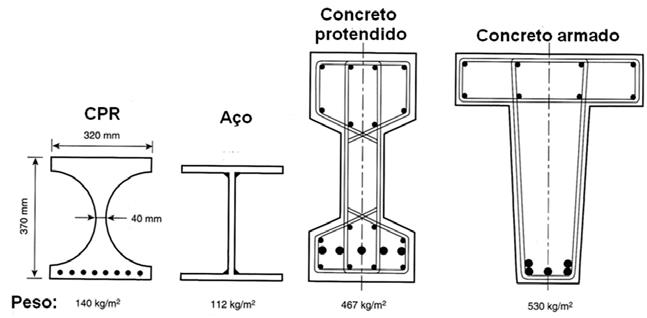
\includegraphics[max width=\textwidth]{cuad-secao.png}
	\end{center}
	\fonte{\apudonline[p.~1320]{Walraven}{Tutikian}}
\end{figure}

\citeonline[p.~803]{Racky} ainda aponta uma economia a longo prazo, que inclui a manutenção, reparo e demolição da construção, já que o custo do ciclo de vida do empreendimento não se encerra na construção, mas continua por toda sua vida útil.

E não só construções novas se beneficiam do desempenho do CUAD: \citeonline{Piotro} demonstram que, apesar do investimento inicial ser maior ao se optar por uma solução em CUAD, seu uso para recuperar estruturalmente uma ponte causa uma economia em custos de manutenção em comparação com a mesma solução em concreto convencional.

\section{CUAD no mundo}

Muitas construções já foram feitas com CUAD em diversos países. O Canadá, pioneiro na utilização do material ainda em 1997, possui mais de 26 construções, entre pontes, passarelas e viadutos \cite{Russel_e_Graybeal}. A \autoref{construcoes-cuad} lista algumas construções feitas em CUAD ao redor do mundo.

\begin{table}[htb]
\IBGEtab{%
  \caption{Exemplos de aplicações de CUAD ao redor do mundo.}
  \label{construcoes-cuad}
}{%
  \begin{tabulary}{\linewidth}{CCCCCC}
  \toprule
   Estruturas/aplicações & Local & Ano & Resistência à compressão (MPa) & Resistência à flexão (MPa) \\
  \midrule \midrule

   Passarela Sherbrooke	           & Sherbrooke, Canadá      & 1997 & 200 &	40	\\ \midrule 
   Silo de clínquer Joppa	       & Illinois, EUA           & 2001 & 220 &	50	\\ \midrule 
   Passarela Seonyu	               & Seul, Coréia do Sul     & 2002 & 180 &	32	\\ \midrule 
   Passarela Sakata Mirai	       & Sakata, Japão           & 2002 & 238 &	40	\\ \midrule 
   Pedágio no Millau Viaduct	   & Rodovia A75, França     & 2002 & 165 &	30	\\ \midrule 
   Ponte da angra Sheperds	       & Sydney, Austrália       & 2005 & 180 &	-	\\ \midrule
   Painéis resistentes a explosão  & Melbourne, Australia    & 2005 & 160 & 30  \\ \midrule 
   Passarela Papatoetoe	           & Auckland, Nova Zelândia & 2006 & 160 &	30	\\ \midrule 
   Ponte Glenmore/Legsby	       & Calgary, Canadá         & 2007 & -	  &	-	\\ \midrule 
   Ponte Gaertnerplatz	           & Kassel, Alemanha        & 2007 & 150 &	35	\\ \midrule 
   Ponte Jakway Park               & Iowa, EUA               & 2008 & 150 &	-	\\ \midrule 
   Fundações de turbina eólica	   & Dinamarca               & 2008 & 210 &	24	\\ \midrule
   Lajes do Aeroporto de Haneda	   & Tóquio, Japão           & 2010 & 210 & 45	\\ \midrule 
   Ponte Whiteman Creek	           & Brantford, Canadá       & 2011 & 140 & 30	\\ \midrule
   Canos de esgoto                 & Alemanha                & 2012 & 151 & –   \\ \midrule
   Colunas do tipo "spun"          & Alemanha                & 2012 & 179 & –   \\ \midrule
   Passarela de treliças de CUAD   & Espanha                 & 2012 & 150 & –	\\
  \bottomrule
\end{tabulary}%
}{%
  \fonte{\citeonline[p.~273.]{Abbas}.}%
  %\nota{Esta é uma nota, que diz que os dados são baseados na regressão linear.}
  %\nota[Anotações]{Uma anotação adicional, que pode ser seguida de várias outras.}
  }
\end{table}

Segundo \citeonline{Russel_e_Graybeal}, a Alemanha iniciou, em 2005, um programa com 34 projetos de pesquisa divididos entre 20 instituições, de modo a desenvolver a base necessária para os estudos técnicos sobre CUAD e torná-lo ``um produto confiável, disponível rotineiramente, economicamente acessível e regularmente aplicado''.

Desde a publicação das recomendações para usar CUAD em estruturas na França \cite{AFGC}, em 2002 (revisada em 2013), muitas pontes já foram executadas. O Japão \cite{JSCE} também publicou um conjunto similar de recomendações em 2006 \cite{Russel_e_Graybeal}.

A Coréia do Sul está pesquisando o uso de CUAD em pontes estaiadas, mostrando que esse material ganha cada vez mais atenção internacional \cite{Russel_e_Graybeal}.

%\section{{CUAD} disponível no mercado} -> [Capítulo removido]

\citeonline{Resplendino} lista os principais concretos de ultra alto desempenho disponíveis no mercado:

\begin{alineas}[label=\textbullet]
  \item Ductal\textsuperscript{\textregistered}, marca comercial do CPR, comercializado pela Lafarge (França);
  \item BSI/CERACEM\textsuperscript{\textregistered}, desenvolvido pelo grupo EIFFAGE SIKA (França);
  \item BCV\textsuperscript{\textregistered}, desenvolvido pelo grupo Vicat (França);
  \item CEMTECmultiscale\textsuperscript{\textregistered}, desenvolvido pela LCPC (França);
  \item Materiais laboratoriais desenvolvidos pela EDF (\textit{Électricité de France}, companhia elétrica francesa), do CERIB (\textit{Centre d’Études et de Recherches de l’Industrie du Béton}, em português: Centro de Estudos e Pesquisas da Indústria do Concreto) (França);
  \item CRC, sob a marca comercial Densit\textsuperscript{\textregistered}, desenvolvido pela Aalborg Portland Cement (Dinamarca);
\end{alineas}

Ainda existe o COR-TUF\textsuperscript{\textregistered} \cite{Durst}, desenvolvido pelo \textit{US Army Corps of Engineers Engineer Research and Development Center} (em português, Centro de Pesquisa e Desenvolvimento de Engenharia do Corpo de Engenheiros do Exército dos Estados Unidos), o qual ainda procura parceiros comerciais para licenciar e comercializar o COR-TUF\textsuperscript{\textregistered}. Outro CUAD que pode ser encontrado no mercado é o DURA\textsuperscript{\textregistered} \cite{Dura}, produzido por uma empresa de mesmo nome, na Malásia.

\section{CUAD no Brasil}

No Brasil, já é possível encontrar o Ductal\textsuperscript{\textregistered} na fachada de dois edifícios na cidade de São Paulo: no edifício do Escritório de Representação do Ministério das Relações Exteriores (\autoref{fachada_ministerio_1} e \autoref{fachada_ministerio_2}) e na fachada da Japan House (\autoref{fachada_japan_house_1} e \autoref{fachada_japan_house_2}).

\begin{figure}[htb]
	\caption{\label{fachada_ministerio_1}Fachada executada com o CUAD Edifício do Escritório de Representação do Ministério das Relações Exteriores, na Rua da Consolação, São Paulo – SP.}
	\begin{center}
	    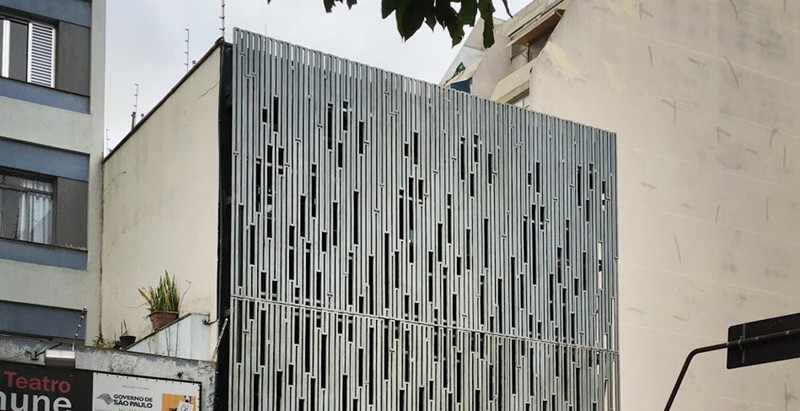
\includegraphics[max width=\textwidth]{fachada-ministerio-1.jpg}
	\end{center}
	\fonte{\citeonline{Stone}.}
\end{figure}

\begin{figure}[htb]
	\caption{\label{fachada_ministerio_2}Detalhe da fachada do mesmo edifício da \autoref{fachada_ministerio_1}.}
	\begin{center}
	    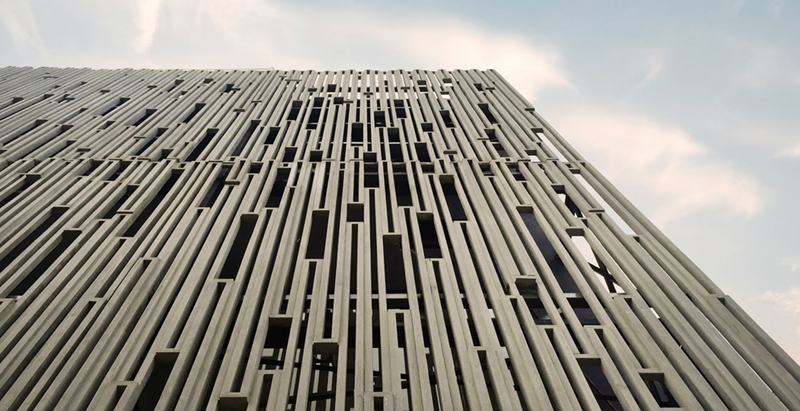
\includegraphics[max width=\textwidth]{fachada-ministerio-2.jpg}
	\end{center}
	\fonte{\citeonline{Stone}.}
\end{figure}

\begin{figure}[htb]
	\caption{\label{fachada_japan_house_1}Fachada executada com CUAD. Japan House, na Avenida Paulista, São Paulo - SP.}
	\begin{center}
	    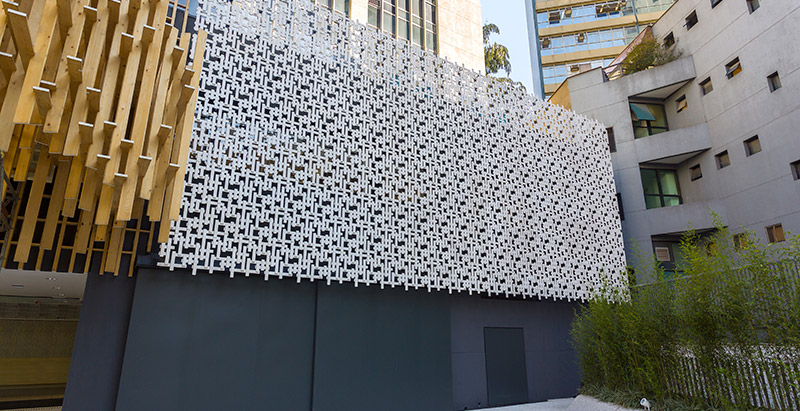
\includegraphics[max width=\textwidth]{fachada-japan-house-1.jpg}
	\end{center}
	\fonte{\citeonline{Stone}.}
\end{figure}

\begin{figure}[htb]
	\caption{\label{fachada_japan_house_2}Detalhe da mesma fachada da \autoref{fachada_japan_house_1}}
	\begin{center}
	    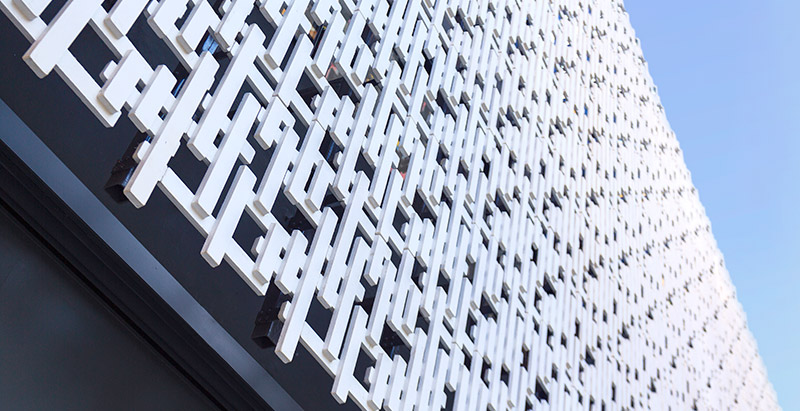
\includegraphics[max width=\textwidth]{fachada-japan-house-2.jpg}
	\end{center}
	\fonte{\citeonline{Stone}.}
\end{figure}

%\begin{figure}[htb]
%	\caption{\label{pulaski_skyway}Ponte Pulaski Skyway, New Jersey, EUA. Construída com CUAD.}
%	\begin{center}
%	    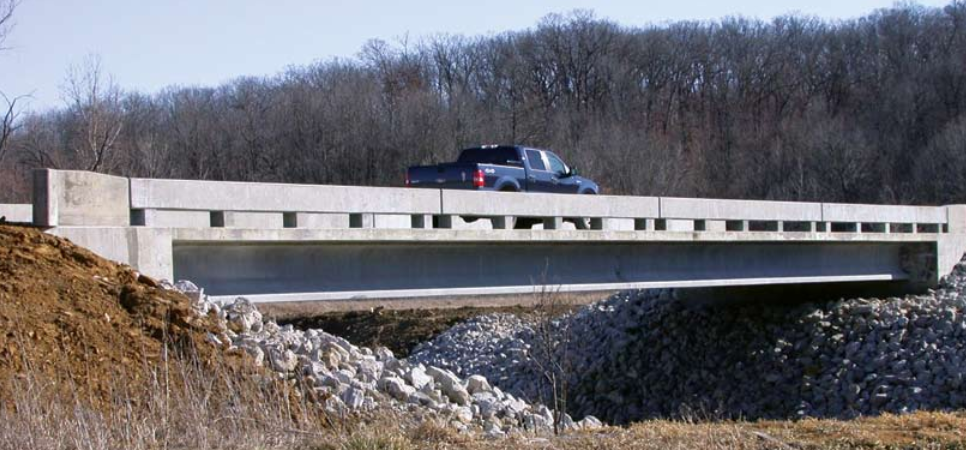
\includegraphics[max width=\textwidth]{ponte-pulaski-skyway.png}
%	\end{center}
%	\fonte{\citeonline{Stone}.}
%\end{figure}
\chapter{Projetos em CUAD}

Para elaborar projetos com concreto de ultra alto desempenho, é imprescindível ter em mente que as características inerentes do material possibilitam a exploração de novos métodos e geometrias de construção que otimizem e justifiquem seu uso em detrimento dos métodos tradicionais de construção. Apesar disso, com exceção da passarela de Sherbrooke (\autoref{chap:sher}), nenhuma das estruturas feitas com CUAD possuem um projeto topológico drasticamente diferente do utilizado em estruturas de concreto convencional \cite[p.~603]{Flint}.

%\citeonline{Flint} sugerem o uso de algoritmos como ``otimização da colônia da formiga'' que, através de diversas iterações, procura chegar à uma solução ótima de caminho mínimo de distribuição de cargas para um determinado problema estrutural. Aplicando-se outros algoritmos e inteligência artificial também pode ocasionar na descoberta de topologias diferentes e inovadoras que se encaixem na proposta de uso do CUAD e que, de outra maneira, poderiam não ser consideradas pelo projetista. É importante salientar que as soluções computacionais ainda precisam ser interpretadas e desenvolvidas de maneira apropriada por um engenheiro competente.

A computação já inspira arquitetos e engenheiros a desenvolverem soluções de arquitetura e engenharia inovadoras, e o CUAD permite a aplicação desses projetos com muito mais facilidade que o aço, possuindo um desempenho muito próximo, mas com uma grande vantagem: a indústria do aço é muito refinada, e seu processo de produção consome muito mais energia e emite muito mais gases poluentes que a indústria do concreto. Outra vantagem que o CUAD leva sobre o aço é a durabilidade, já que sem um tratamento especial e manutenção cuidadosa, o aço se deteriora rapidamente. Por último, oferece um grande desempenho para estruturas comparativamente leves, não sendo um material exótico como fibra de carbono, por exemplo \cite[p.~11]{Davila}.

Atualmente, o CUAD encontra-se em uma fase experimental de adoção, pois ainda não existe um manual que apresente ao engenheiro de estruturas que critérios e elementos são necessários para projeto, além de exemplos claros de implementação. As informações ainda encontram-se espalhadas e os projetos existentes ainda exigem uma análise cuidadosa, caso a caso, o que muita vezes faz com que o responsável pelo projeto adote soluções mais conservadoras, sub-utilizando a capacidade do material. Ainda é preciso um grande trabalho de pesquisa e divulgação do CUAD para que isso seja produzido para o grande público \cite[p.~13]{Davila}.

Mesmo que o CUAD permita a construção de estruturas mais leves e esbeltas, é preciso ter cuidado com a geometria escolhida, além do cuidado com a deformação da peça, já que o seu módulo de elasticidade é apenas duas vezes maior que o do concreto convencional.

As próximas seções mostram os cuidados necessários para trabalhar com o CUAD e alguns exemplos de obras executadas em CUAD, das primeiras às mais recentes.

%Resplendino
%713 Recomenda fucking ções

%Resplendino fachadas
%405

\section{Métodos construtivos para CUAD}

Para se atingir as altas resistências desejadas no CUAD, é imprescindível um rigoroso controle tecnológico dos materiais utilizados na fabricação do CUAD. A adição de fibras em grandes volumes de concreto é por si só problemática, pois não é possível controlar sua distribuição na mistura e sua correta dispersão é altamente desejável para que elas trabalhem a favor da resistência do concreto, e não se acumulem em apenas um local.

A mistura dos materiais pode ser feita de diversas formas, desde que se observe com cuidado a distribuição das fibras. O próximo passo, crucial para que as resistências desejadas sejam atingidas é a cura do concreto, que deve ser feita em ambiente saturado de vapor e, preferencialmente, sob pressão (cura em autoclave), pois isso irá melhorar ainda mais a resistência do CUAD.

Este processo só pode ser controlado corretamente em um ambiente industrializado, de modo que não se recomenda a utilização de CUAD moldado \textit{in loco}, por conta da dificuldade do controle tecnológico do concreto em um ambiente aberto.

\section{Aplicações}
\label{chap:obras-cad}

\subsection{Passarela de Sherbrooke, Canadá}
\label{chap:sher}

A passarela de Sherbrooke (\autoref{sherbrooke}), construída sobre o rio Magog, na cidade de Quebec, Canadá, foi a primeira estrutura construída inteiramente com concreto de pós reativos (CPR), uma variedade de concreto de ultra alto desempenho (CUAD), sem a utilização de barras de aço. Sua superestrutura consiste de treliças de CPR com com uma resistência característica de 200 MPa confinadas em tubos de aço inoxidável sobre um vão de 60 metros \cite[p.~140]{Aitcin_sher}.

\begin{figure}[htb]
	\caption{\label{sherbrooke}Passarela de Sherbrooke, Quebec, Canadá. Construída em CPR (concreto de pós reativos) sem o uso de barras de aço.}
	\begin{center}
	    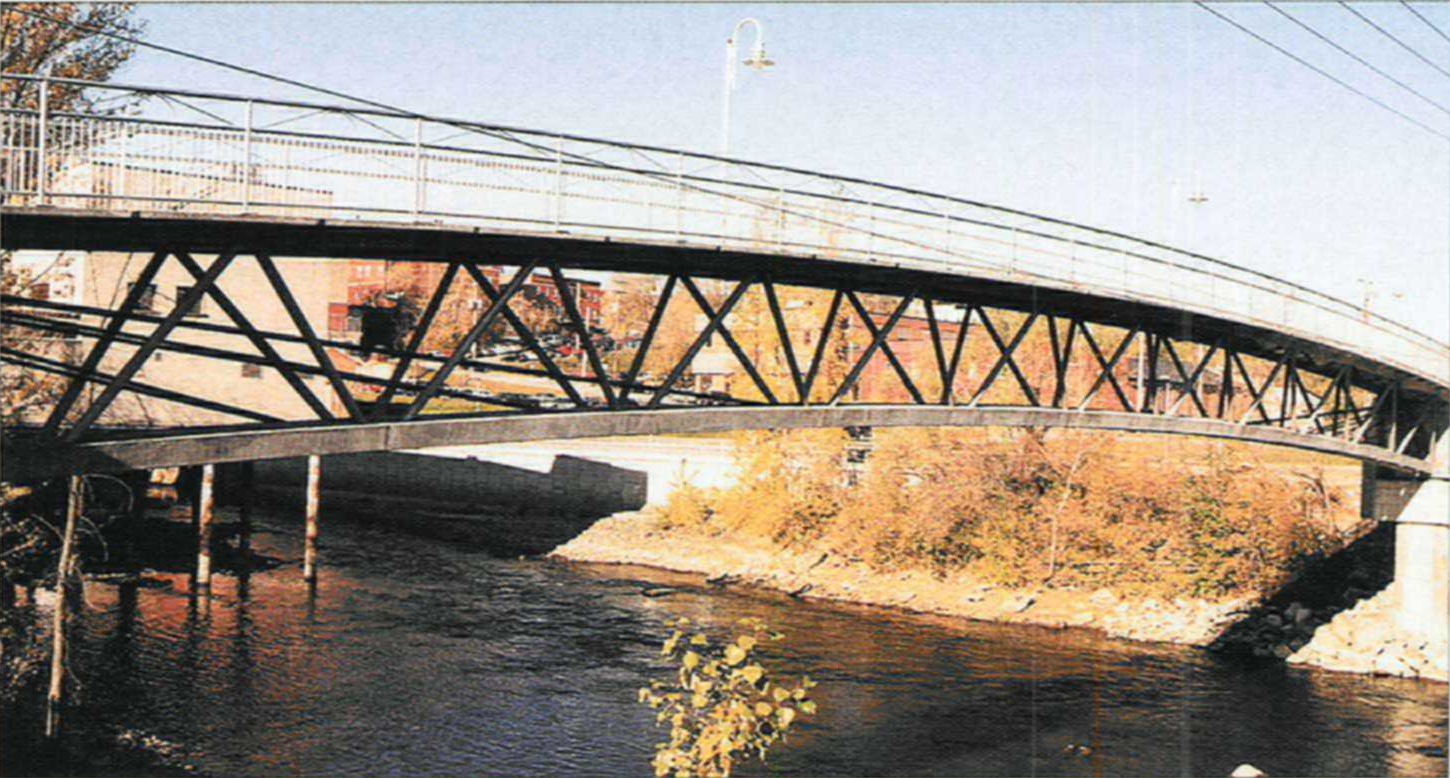
\includegraphics[max width=\textwidth]{sherbrooke.png}
	\end{center}
	\fonte{\citeonline[p.~140]{Aitcin_sher}.}
\end{figure}

As partículas utilizadas no CPR utilizado para construir a passarelas foram limitadas a 0,8 mm. Sua mistura consiste em cimento Portland, fumo de sílica, pó de quartzo, areia, superplastificante, água e fibras de aço com resistência de 2600 MPa, 0,2 mm de diâmetro e 13 mm de comprimento. A mistura foi confinada em tubos de aço inoxidável de 150 mm de diâmetro e espessura de 2 mm. Este confinamento serve para transformar a ruptura frágil apresentada pelo CUAD em uma ruptura pseudo-dúctil, além de melhorar ainda mais as suas propriedades mecânicas, incluindo a  capacidade de suportar uma solicitação de compressão de 350 MPa \citeonline[p.~141]{Aitcin_sher}. A \autoref{sherbrooke_traco} mostra o traço de CPR utilizado na passarela de Sherbrooke. Já a \autoref{sherbrooke_curva} mostra as curvas de tensão-deformação compressivas para diferentes tipos de concretos testados na época da construção da ponte. No gráfico, é possível observar um considerável aumento na resistência à compressão de um mesmo CPR em três condições distintas (livre, confinado e confinado e comprimido). A curva de tensão-deformação do CAD aparece apenas para se fazer um comparativo.

\begin{table}[htb]
\IBGEtab{%
  \caption{Dosagem do CPR usado na passarela de Sherbrooke.}
  \label{sherbrooke_traco}
}{%
  \begin{tabulary}{\linewidth}{CCC}
  \toprule
   Material                 & Quantidade    \\
  \midrule \midrule
   Cimento                  & 705 $\text{kg/m}^3$  \\ \midrule 
   Fumo de sílica           & 230 $\text{kg/m}^3$  \\ \midrule 
   Pó de quartzo            & 210 $\text{kg/m}^3$  \\ \midrule 
   Areia                    & 1010 $\text{kg/m}^3$ \\ \midrule 
   Superplastificante       & 37,5 $\text{l/m}^3$  \\ \midrule 
   Fibras de aço            & 190 $\text{kg/m}^3$  \\ \midrule 
   Água (a/c = 0,21)        & 195 $\text{l/m}^3$   \\
  \bottomrule
\end{tabulary}%
}{%
  \fonte{\citeonline[p.~141]{Aitcin_sher}.}%
  %\nota{Recomenda-se o uso de água de amassamento de baixa temperatura, pré cura térmica de 2 dias e cura térmica de 24 horas a uma temperatura de 80\textsuperscript{\degree} C.}
  %\nota[Anotações]{Uma anotação adicional, que pode ser seguida de várias outras.}
  }
\end{table}

\begin{figure}[htb]
	\caption{\label{sherbrooke_curva} Curvas de tensão-deformação compressivas para diferentes concretos.}
	\begin{center}
	    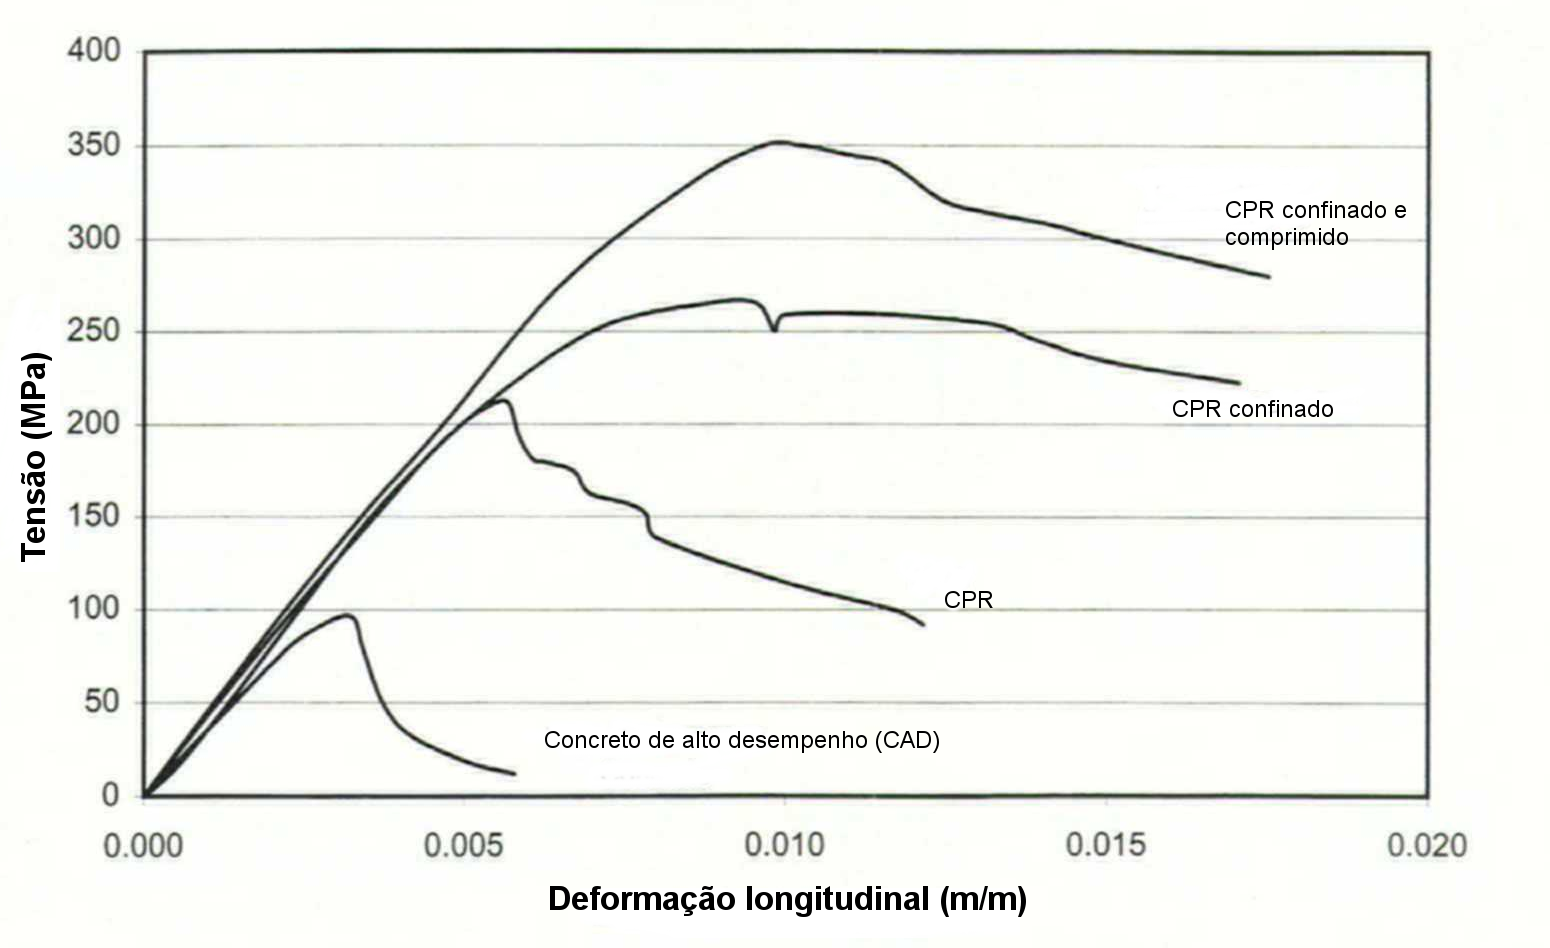
\includegraphics[max width=\textwidth]{sherbrooke-strain.png}
	\end{center}
	\fonte{\citeonline[p.~141]{Aitcin_sher}.}
\end{figure}

Para o projeto da passarela, foram feitas as seguintes considerações: resistência à compressão de 180 MPa, resistência à tração direta de 7 MPa, resistência à flexão de 40 MPa e módulo de elasticidade de 50 GPa. Através de um processo rigoroso de produção introduzido na fábrica de pré-moldados onde a passarela foi moldada, compressão do CPR ainda fresco e cura térmica a vapor, a uma temperatura de 90\textsuperscript{\degree} C, o material foi capaz de atingir uma resistência média de 200 MPa, aferida em corpos de prova recolhidos em diferentes lotes de produção de CPR \cite[p.~141]{Aitcin_sher}.

A passarela possui um tabuleiro de 30 mm de espessura, protendido transversalmente e longitudinalmente e não possui reforço passivo de aço. Por motivos de segurança, o potencial do material não foi explorado completamente, já que esta foi a primeira experiência de uso do material em uma obra aberta ao público \cite[p.~141]{Aitcin_sher}. A seção transversal e longitudinal pode ser vista na \autoref{cross-section} e na \autoref{longitudinal}, respectivamente. A \autoref{precast} mostra um segmento pré-moldado finalizado da ponte, ainda na fábrica.

\begin{figure}[htb]
	\caption{\label{cross-section} Corte transversal da passarela de Sherbrooke.}
	\begin{center}
	    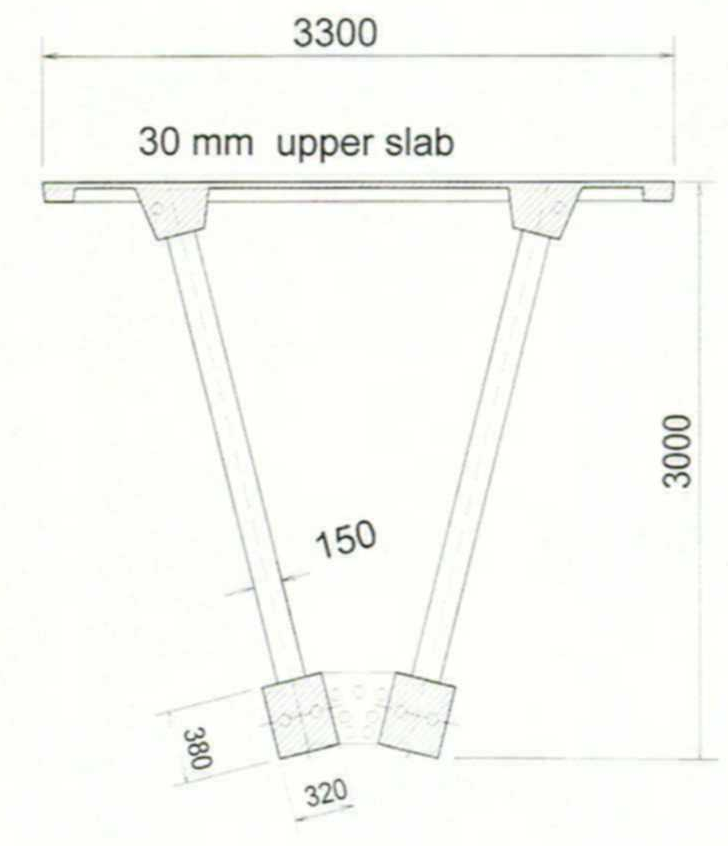
\includegraphics[max width=4cm]{cross-section.png}
	\end{center}
	\fonte{\citeonline[p.~141]{Aitcin_sher}.}
\end{figure}

\begin{figure}[htb]
	\caption{\label{longitudinal}Elevação da passarela de Sherbrooke mostrando a protensão longitudinal.}
	\begin{center}
	    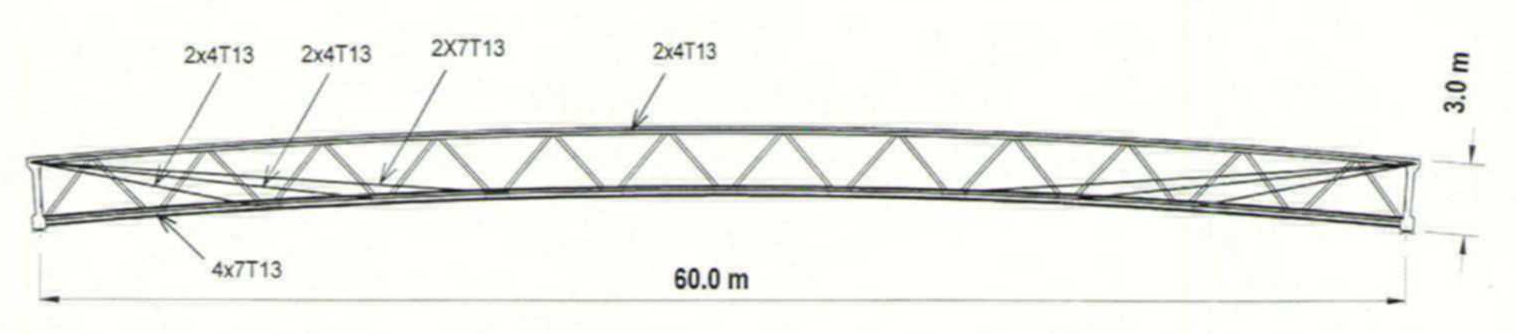
\includegraphics[max width=\textwidth]{longitudinal-prestressing.png}
	\end{center}
	\fonte{\citeonline[p.~142]{Aitcin_sher}.}
\end{figure}

\begin{figure}[htb]
	\caption{\label{precast}Segmento pré-moldado finalizado da passarela.}
	\begin{center}
	    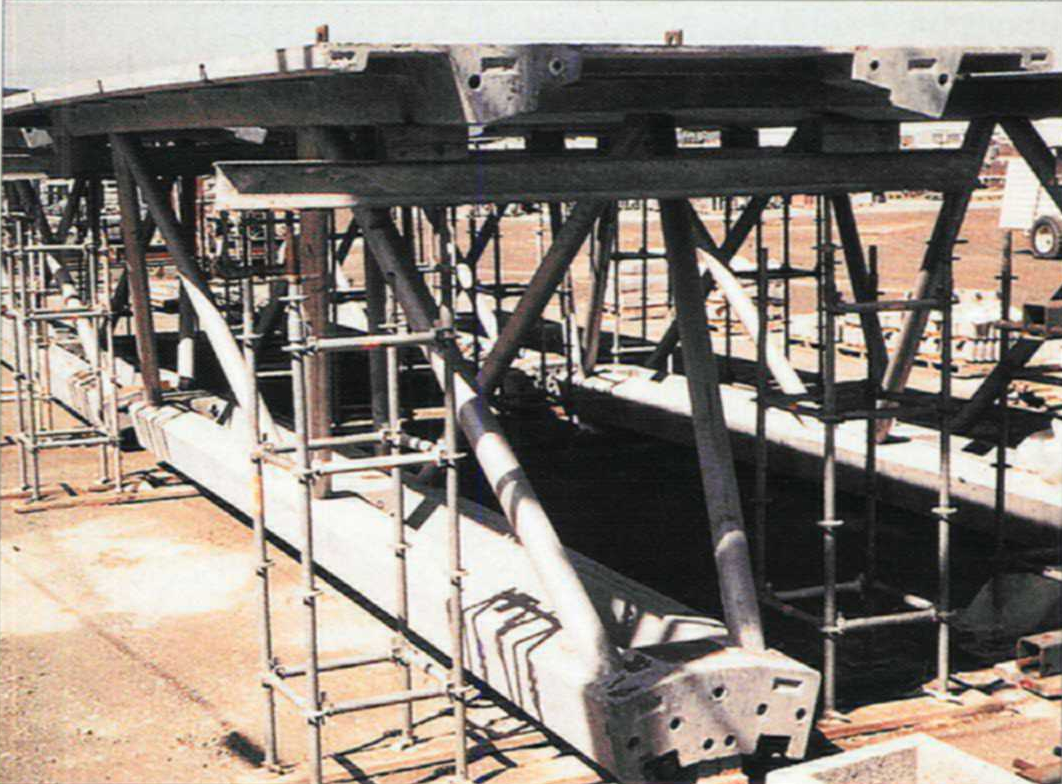
\includegraphics[max width=\textwidth]{precast.png}
	\end{center}
	\fonte{\citeonline[p.~142]{Aitcin_sher}.}
\end{figure}
\subsection{Passarela sobre a ravina de Ovejas, Espanha}

A passarela sobre a ravina de Ovejas, província de Alicante, Espanha é uma passarela de 45 metros (\autoref{ovejas} e \autoref{ovejas-2}), protendida, feita com treliças do tipo Warren de CUAD (\autoref{ovejas-long} e \autoref{ovejas-bottom}). Foi a primeira passarela feita completamente com treliças de CUAD. A espessura do tabuleiro é de apenas 3 cm e a resistência do concreto é de 150 MPa. A \autoref{ovejas-section} e a \autoref{ovejas-section-2} mostram a configuração  da passarela com mais detalhes.

\begin{figure}[htb]
	\caption{\label{ovejas}Passarela sobre a ravina de Ovejas, Província de Alicante, Espanha.}
	\begin{center}
	    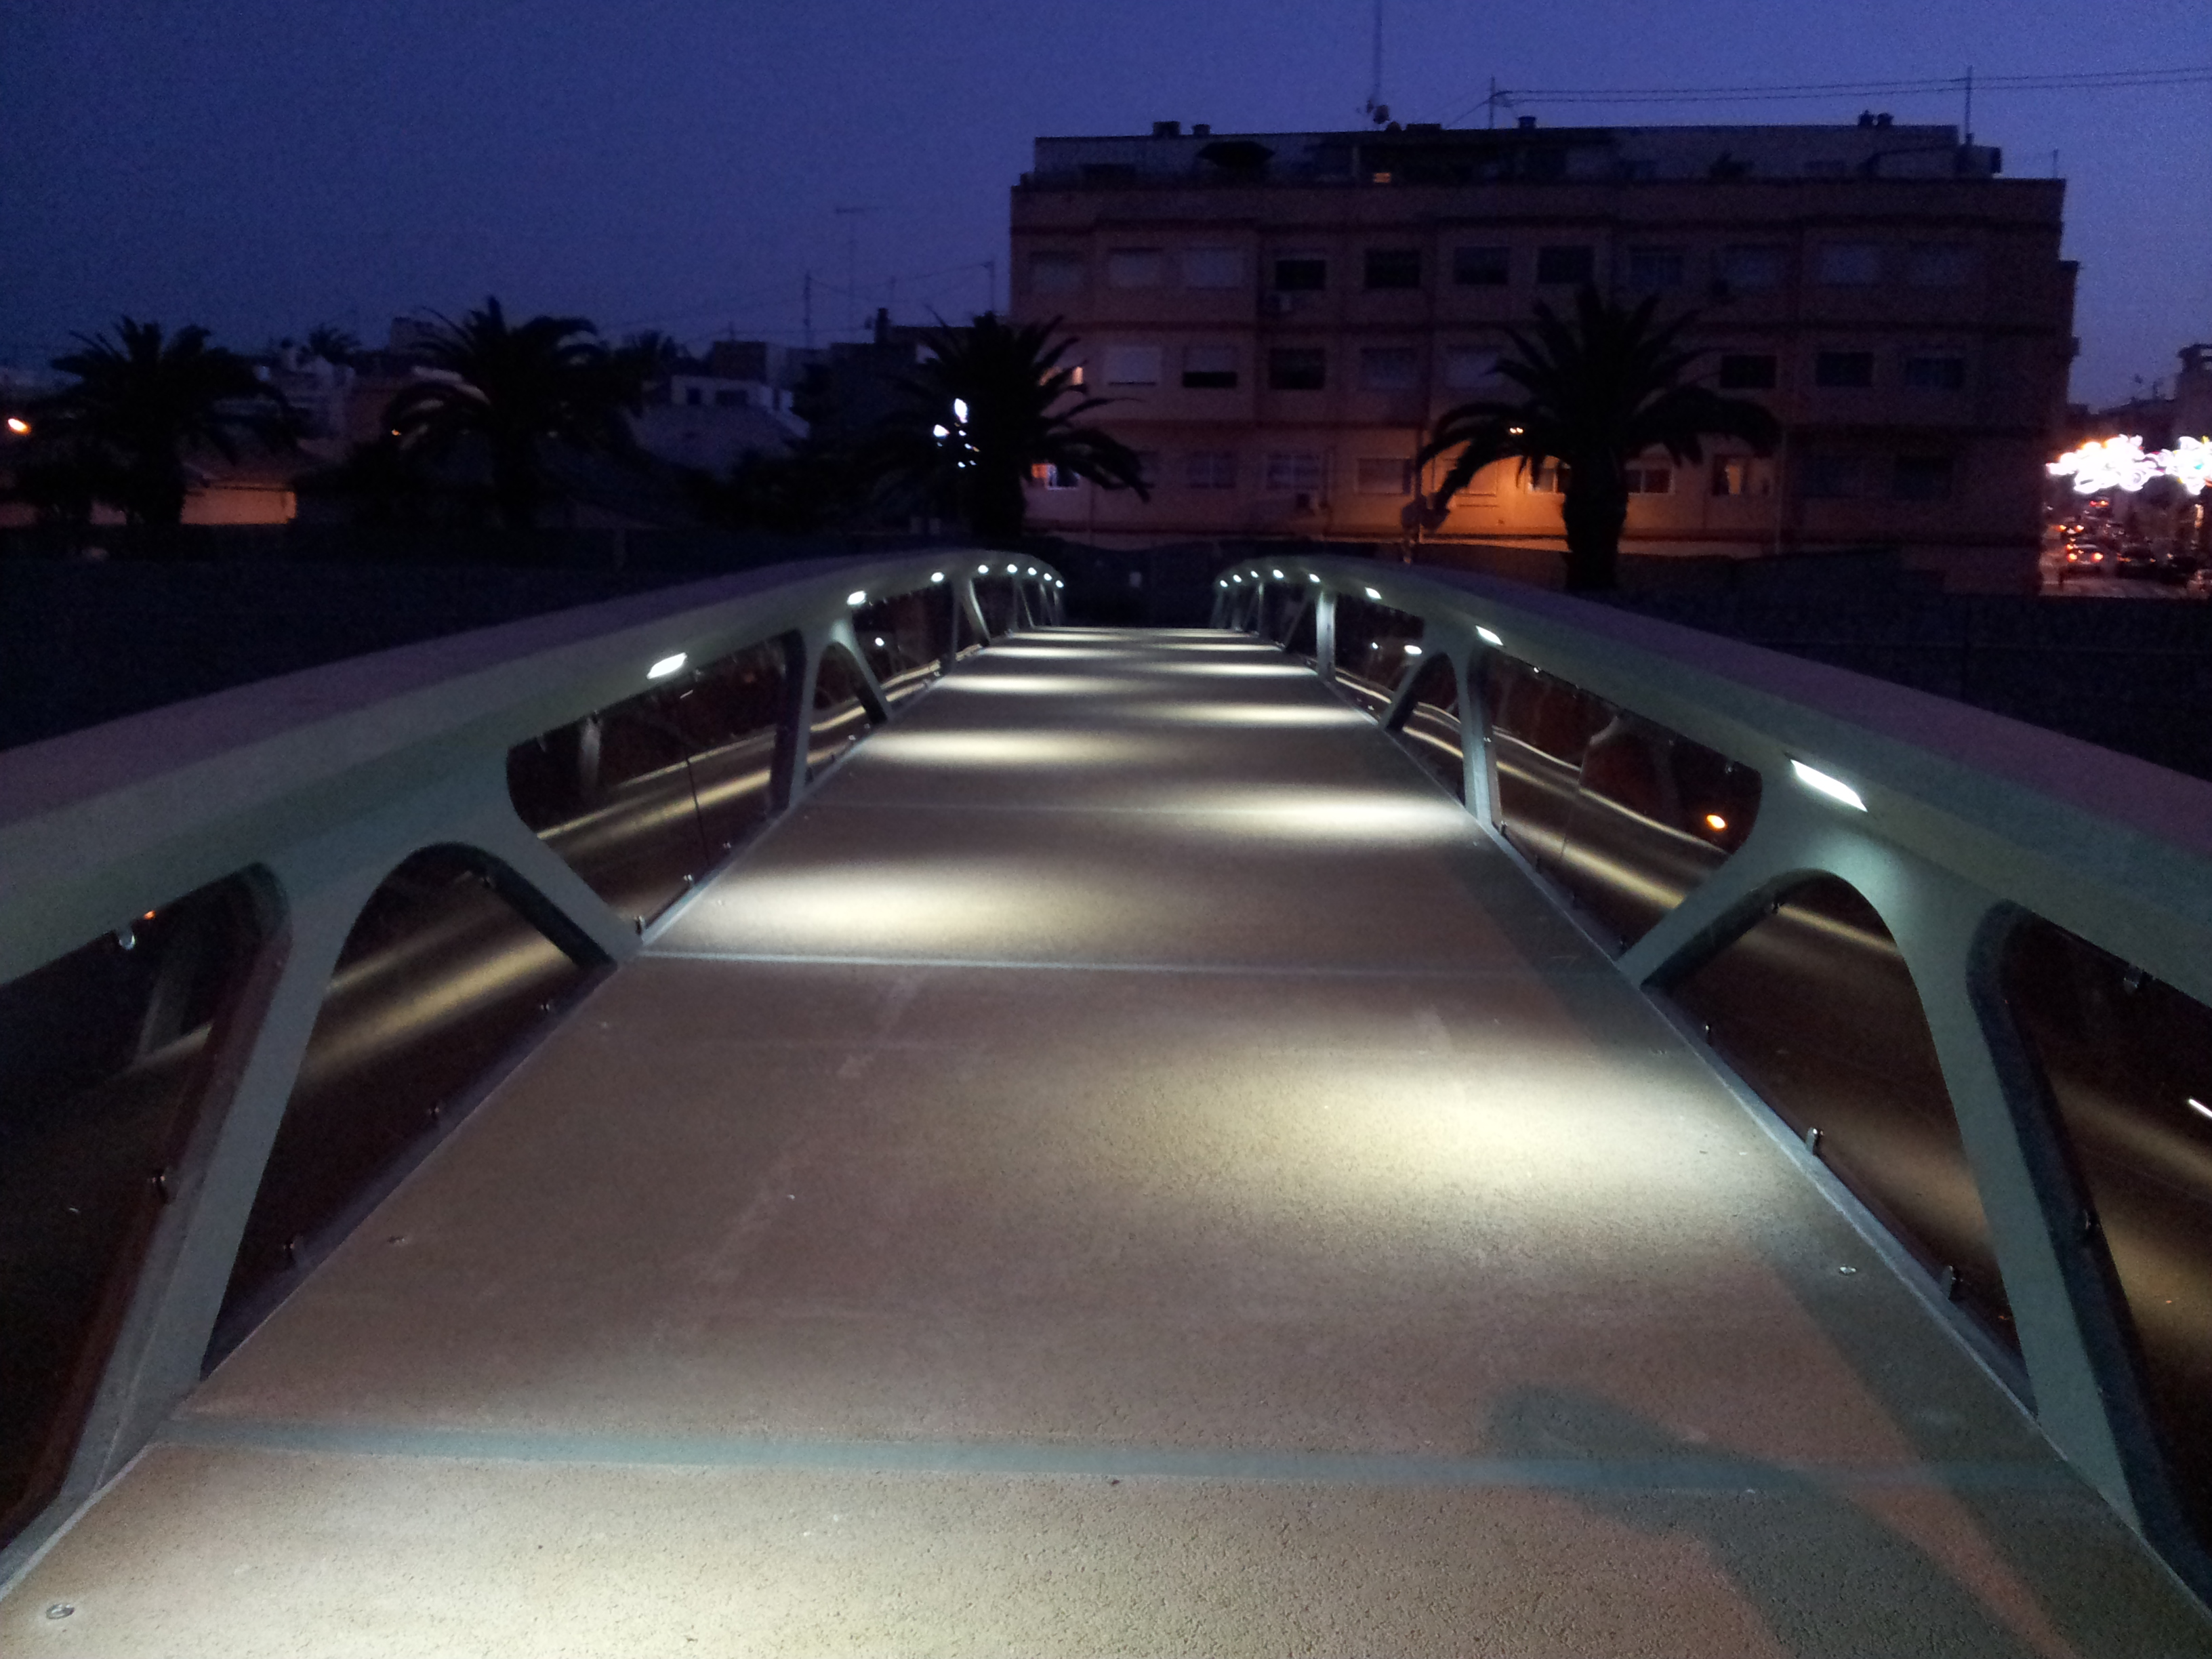
\includegraphics[max width=\textwidth]{passarela-ovejas.jpg}
	\end{center}
	\fonte{\citeonline{RDC}}
\end{figure}

\begin{figure}[htb]
	\caption{\label{ovejas-2}Representação gráfica da passarela de Ovejas.}
	\begin{center}
	    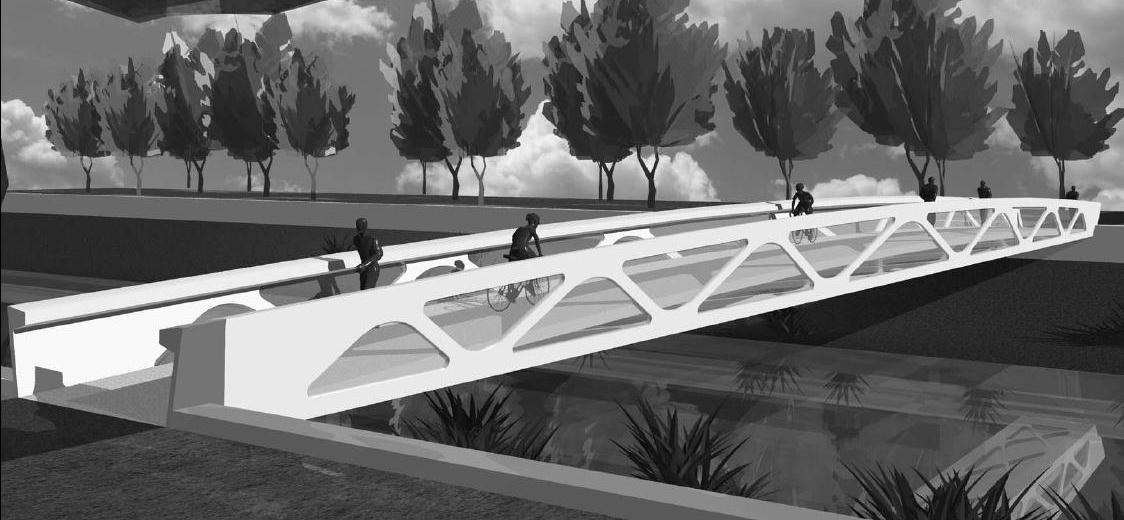
\includegraphics[max width=\textwidth]{ovejas-overview.png}
	\end{center}
	\fonte{\citeonline{Lopez}}
\end{figure}

\begin{figure}[htb]
	\caption{\label{ovejas-long}Vista longitudinal da passarela.}
	\begin{center}
	    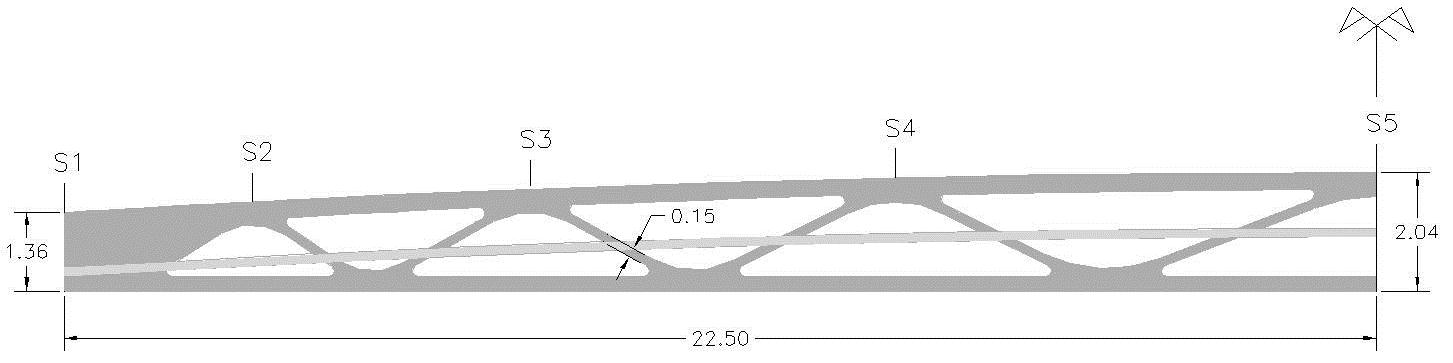
\includegraphics[max width=\textwidth]{ovejas-longitudinal.png}
	\end{center}
	\fonte{\citeonline{Lopez}}
\end{figure}

\begin{figure}[htb]
	\caption{\label{ovejas-bottom}Treliças abaixo do tabuleiro.}
	\begin{center}
	    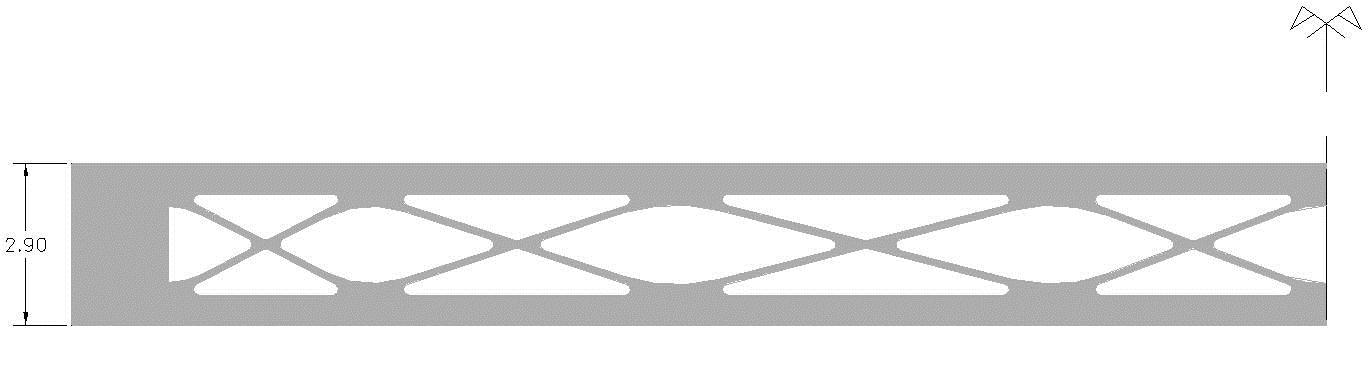
\includegraphics[max width=\textwidth]{ovejas-bottom.png}
	\end{center}
	\fonte{\citeonline{Lopez}}
\end{figure}

\begin{figure}[htb]
	\caption{\label{ovejas-section} Corte transversal da passarela com detalhamento.}
	\begin{center}
	    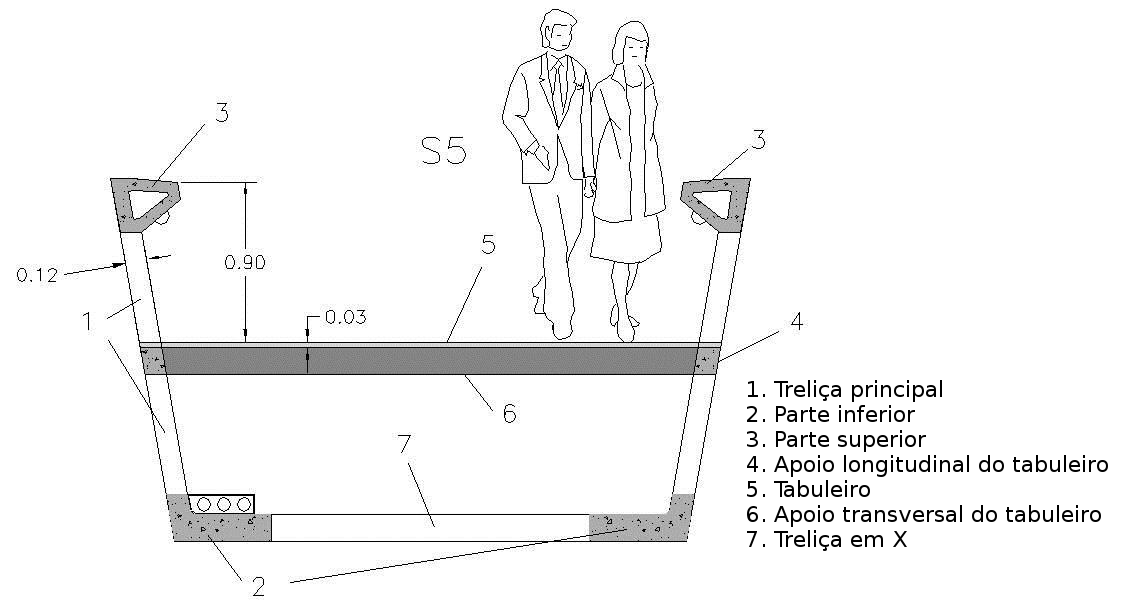
\includegraphics[max width=\textwidth]{ovejas-corte.png}
	\end{center}
	\fonte{\citeonline{Lopez}}
\end{figure}

\begin{figure}[htb]
	\caption{\label{ovejas-section-2}Corte transversal da passarela com detalhamento.}
	\begin{center}
	    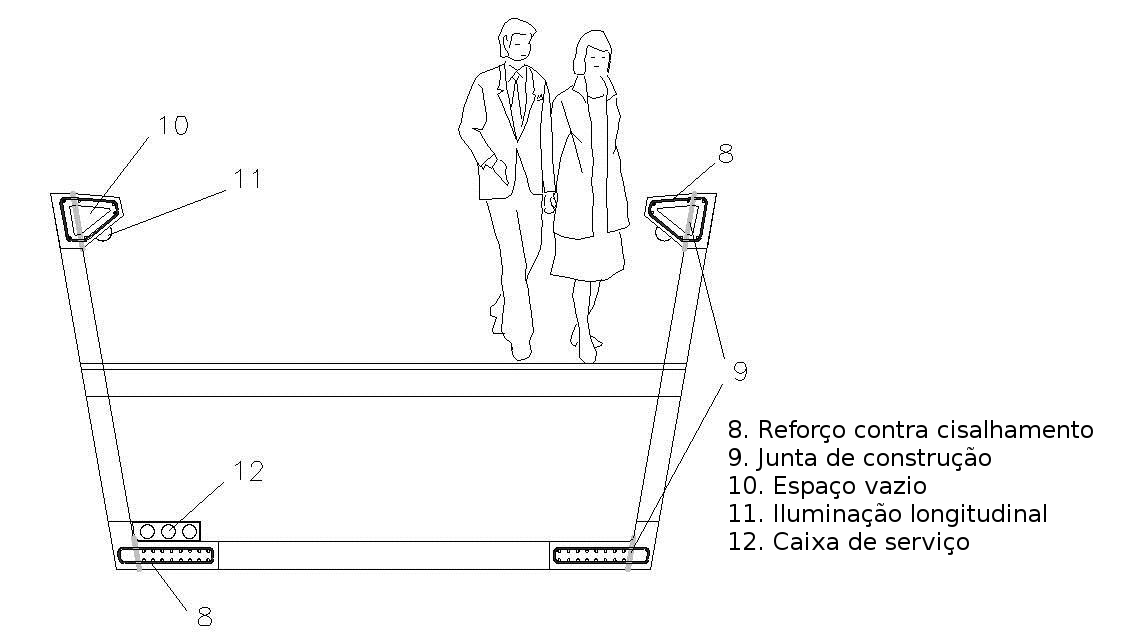
\includegraphics[max width=\textwidth]{ovejas-corte2.png}
	\end{center}
	\fonte{\citeonline{Lopez}}
\end{figure}

A passarela foi moldada na fábrica e transportada por inteiro para sua locação final. O estudo do carregamento da estrutura foi feito com o software SAP2000, considerando as ações especificadas na \autoref{ovejas-acoes}. O traço de concreto utilizado é mostrado na \autoref{ovejas-traco}.


\begin{table}[htb]
	\IBGEtab{%
		\caption{Ações consideradas no projeto da passarela.}
		\label{ovejas-acoes}
		}{%
		\begin{tabulary}{\linewidth}{CC}
			\toprule
			Propriedade                                    & Valor \\
			\midrule \midrule
			Peso próprio                                   & 4,3 kN/m\textsuperscript{2} \\ \midrule
			Carregamento dinâmico característico	       & 5,0 kN/m\textsuperscript{2} \\ \midrule
			Carregamento dinâmico frequente                & 2,0 kN/m\textsuperscript{2} \\ \midrule
			Deformação vertical sob carregamento frequente & 3,6 cm                      \\ \midrule
			Velocidade básica do vento	                   & 18 m/s                      \\ \midrule
			Temperatura mais alta	                       & 34,2\textsuperscript{\degree}C   \\ \midrule
			Temperatura mais baixa                         & 11,5\textsuperscript{\degree}C    \\ \midrule 
			Aceleração sísmica máxima horizontal/vertical  & 3,44/2,41 m/s\textsuperscript{2} \\
			\bottomrule
		\end{tabulary}%
	}{%
	\fonte{\citeonline[p.~899]{Lopez}.}%
			%\nota{Esta é uma nota, que diz que os dados são baseados na regressão linear.}
			%\nota[Anotações]{Uma anotação adicional, que pode ser seguida de várias outras.}
	}
\end{table}

\begin{table}[htb]
	\IBGEtab{%
		\caption{Traço do CUAD utilizado.}
		\label{ovejas-traco}
	}{%
	\begin{tabulary}{\linewidth}{CC}
		\toprule
		Material                                       & Quantidade (kg/m\textsuperscript{3}) \\
		\midrule \midrule
		Cimento (a/c = 0,213)                          & 1000 \\ \midrule
		Fumo de sílica                 	               & 150  \\ \midrule
		Areia 0,5 mm                                   & 702  \\ \midrule
		Areia 1,8 mm                                   & 380  \\ \midrule
		Água                  	                       & 213  \\ \midrule
		Superplastificante \textsuperscript{1}          & 9,06 \\ \midrule
		Fibras OL13/0.16 \textsuperscript{2}            & 78,1 \\ \midrule 
		Fibres RC80/40 BP \textsuperscript{2}           & 78,1 \\
		\bottomrule
	\end{tabulary}%
}{%
\fonte{\citeonline[p.~899]{Lopez}.}%
\nota{\textsuperscript{1)} Fração sólida de superplastificante;}
\nota{\textsuperscript{2)} 1\% em volume de cada fibra de Bekaert.}
%\nota[Anotações]{Uma anotação adicional, que pode ser seguida de várias outras.}
}
\end{table}

%2nd preceedings 45 Ultra-High Performance Concretes – recent realizations and research programs on UHPFRC bridges in France

%2nd preceedings 813 pra frente Muita coisa, não sei se precisa colocar também

%\subsection{Pavimentação}
%1st preceedings 745 Durability and Mechanical Properties of High Performance
%Concrete for Ultra-Thin Whitetopping Pavements

%\subsection{tubos em pontes e prédios}
%1st preceedings 807

%\subsection{Cascas}
%1st preceedings 827 Ultra-High Performance Fibre Reinforced Concret for shells

%2nd preceedings 707 Flexural Behaviour of Fibre Reinforced Ultra High Performance Concrete and the Application in Cladding Panels

\subsection{Ponte Jakway Park}
\label{chap:jakway}

%Para elaborar este estudo de caso, utilizou-se a documentação disponibilizada pelo Departamento de Transporte do estado de Iowa, EUA e pelo e-mail cordialmente enviado pelo engenheiro Brian Keierbeler, com várias informações sobre o projeto da ponte Jakway Park.
%
%Na primeira seção, apresenta-se o processo de concepção do projeto e as motivações que levaram à escolha do CUAD como solução construtiva da ponte. Em seguida, estuda-se uma viga de seção retangular protendida feita com concreto convencional e comparando-a com uma feita em CUAD, calculando a força de protensão inicial exigida em cada uma. Neste trabalho, toma-se a liberdade de extrapolar as equações para cálculo de estruturas de concreto protendido da NBR 6118:2014 para uso em CUAD, já que a própria norma avisa que seus casos de uso são feitos para concretos com $ f_{ck} $ de até 90 MPa. É importante reforçar que ainda não existe normatização para o uso de CUAD em nenhum país, somente as recomendações de uso publicadas pela \cite{AFGC}\footnote{\textit{Association Française de Genie Civil}} e pela \cite{JSCE}\footnote{\textit{Japan Society of Civil Engineers}}, de modo que ainda é preciso desenvolver uma solução própria para cada caso.
%
%Também é importante lembrar que a visita ao empreendimento não foi possível, por conta de se encontrar nos Estados Unidos. Mesmo assim, foi possível observar as características e considerações utilizadas no projeto.
%
%\subsubsection{Características da locação da ponte Jakway Park}

Buchanan, no estado de Iowa, EUA é um município predominantemente rural. \citeonline{Keierleber_email} mostra que as pontes da cidade são muito antigas (muitas construídas entre 1870-1914) e já não são capazes de atender a demanda de veículos atuais. A  \autoref{acidente-1} e a \autoref{acidente-2} retratam acidentes ocorridos no município devido a esta deficiência.

\nomenclature[A]{MIT}{\textit{Massachusetts Institute of Technology}}
\nomenclature[A]{FHWA}{\textit{Federal Highway Administration}}

Como parte de um programa de pesquisa e financiamento através de um programa de construção de pontes inovadoras do governo dos EUA, o município decidiu trocar a velha ponte Jakway Park por uma ponte de CUAD seção $ \pi $, desenvolvida pelo Instituto de Tecnologia de Massachusetts (MIT) e pelo Laboratório Turner-Fairbank da Administração Federal de Rodovias (FHWA) \cite{Keierbeler_et_al}.

\begin{figure}[htb]
	\caption{\label{acidente-1}Acidente em ponte de madeira em Buchanan.}
	\begin{center}
		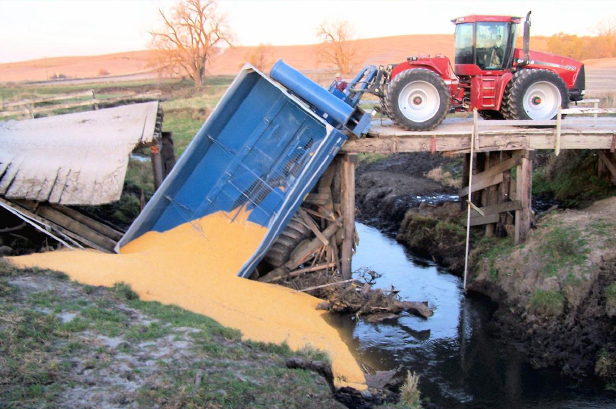
\includegraphics[max width=\textwidth]{acidente-1.png}
	\end{center}
	\fonte{\citeonline{Keierleber_email}}
\end{figure}

\begin{figure}[htb]
	\caption{\label{acidente-2}Acidente em Buchanan.}
	\begin{center}
		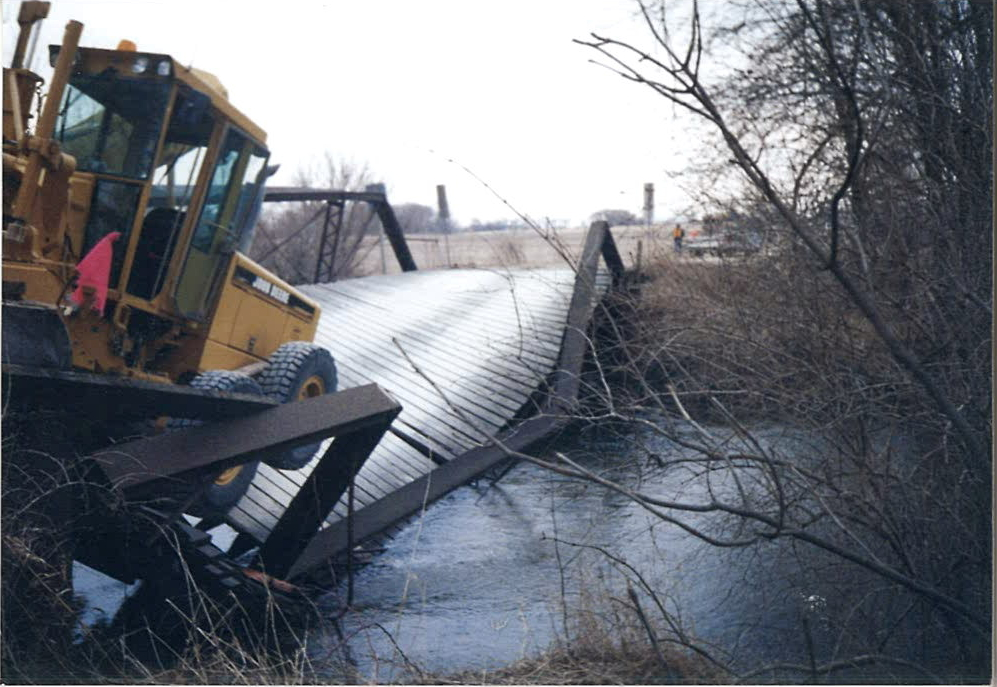
\includegraphics[max width=\textwidth]{acidente-2.jpg}
	\end{center}
	\fonte{\citeonline{Keierleber_email}}
\end{figure}

\subsubsection{Tabuleiro integral de seção \textpi}

O desenvolvimento da seção $ \pi $~começou a ser desenvolvido em 2003 no MIT. O projeto foi otimizado para aproveitar a superior resistência do CUAD para tensão, cisalhamento e compressão, usando a mínima área possível no corte transversal. A primeira geração da seção $ \pi $~(\autoref{secao-pi-1}) falhou nos testes de carregamento, levando os pesquisadores a iterar o projeto \cite[p.~4]{Rouse}. Entre os problemas encontrados, essa geração oferecia um tabuleiro de baixa rigidez, um preocupante comportamento de fissuração com cargas de serviço e problemas na distribuição da carga lateral entre as vigas adjacentes \apud[p.~1]{Graybeal}{Rouse}.

A segunda geração da seção $ \pi $~(\autoref{secao-pi-2}) resolveu os problemas da primeira, sem mudar drasticamente seu desenho, até por questões de economia e reaproveitamento das formas. Com o auxílio do Centro de Engenharia de Pontes (BEC\footnote{\textit{Bridge Engineering Center}}) da Universidade do Estado de Iowa (ISU\footnote{\textit{Iowa State University}}), foi criado um modelo de elementos finitos em 3D no programa ANSYS (\autoref{ansys}). Diversos modelos foram analisados para atender às mudanças necessárias e chegar ao desenho final da nova seção $ \pi $.

Na parte inferior das vigas foi instalado um diafragma metálico, adicionando algum grau de restrição rotacional global no fim das vigas \cite[p.~7]{Rouse}. Cada seção tem uma área de 0,555 m\textsuperscript{2} e um peso próprio de 13,63 kN/m \cite[p.~8]{Rouse}.

Para o dimensionamento das seções que foram utilizadas na construção, limitou-se a resistência a compressão a 148 MPa, por conta do método utilizado para misturar o concreto, o qual foi feito diretamente dentro do caminhão betoneira. Houve o temor que as fibras não se espalhassem da maneira correta, por isso ocorreu essa limitação \cite[p.~8]{Rouse}. A \autoref{valores-de-projeto} lista os dados levados em consideração para o projeto da ponte.

\begin{table}[htb]
	\IBGEtab{%
		\caption{Valores de projeto das propriedades materiais do CUAD.}
		\label{valores-de-projeto}
	}{%
	\begin{tabulary}{\linewidth}{CC}
		\toprule
		Propriedade                                   & Valor (MPa) \\
		\midrule \midrule
		Módulo de elasticidade à liberação            & 39,990 \\ \midrule 
		Módulo de elasticidade final	                 & 53,780 \\ \midrule 
		Resistência de compressão nominal à liberação & 86     \\ \midrule 
		Resistência de compressão nominal final	     & 148    \\ \midrule 
		Resistência nominal à tração final	         & 8,3    \\ \midrule 
		Perda de protensão permitida no escoamento	 & 51,7 (60\% de 86,16 MPa)   \\ \midrule
		Perda de protensão permitida no serviço       & 89   (60\% de 148,33 MPa)  \\ \midrule 
		Tensão de tração permitida no serviço	     & 5,8  (70\% de 8,30 MPa)    \\
		\bottomrule
	\end{tabulary}%
}{%
\fonte{\citeonline[p.~10]{Rouse}.}%
%\nota{Esta é uma nota, que diz que os dados são baseados na regressão linear.}
%\nota[Anotações]{Uma anotação adicional, que pode ser seguida de várias outras.}
}
\end{table}

\begin{figure}[htb]
	\caption{\label{secao-pi-1}Primeira geração da seção $ \pi $.}
	\begin{center}
		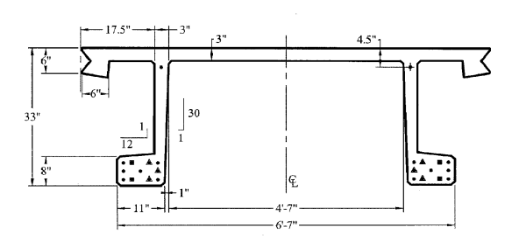
\includegraphics[max width=\textwidth]{secao-pi-1.png}
	\end{center}
	\fonte{\citeonline[p.~5]{Keierleber}}
\end{figure}

\begin{figure}[htb]
	\caption{\label{secao-pi-2}Segunda geração da seção $ \pi $.}
	\begin{center}
		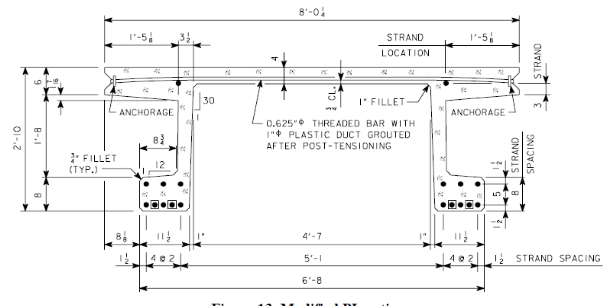
\includegraphics[max width=\textwidth]{secao-pi-2.png}
	\end{center}
	\fonte{\citeonline[p.~10]{Keierleber}}
\end{figure}

\begin{figure}[htb]
	\caption{\label{ansys}Modelo da seção $ \pi $~no ANSYS.}
	\begin{center}
		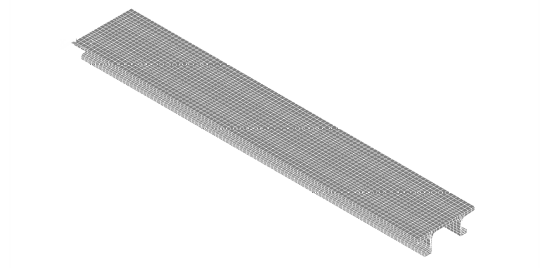
\includegraphics[max width=\textwidth]{ansys.png}
	\end{center}
	\fonte{\citeonline[p.~6]{Rouse}}
\end{figure}

\subsubsection{Construção}

A fornecedora do CUAD utilizado na obra (Lafarge) vende a mistura pronta do concreto. Para fazer o concreto, foi utilizado um caminhão betoneira, misturando o material cimentício, gelo e superplastificantes. Após a homegeinização do concreto, foram adicionadas as fibras de aço com uma peneira, afim de evitar seu agrupamento. Seguiu-se a transferência do CUAD para as formas \autoref{moldagem} e cura térmica a vapor a 90 \textsuperscript{\degree}C por 48 horas (\autoref{vapor}) \cite[p.~17]{Rouse}.

\nomenclature[S]{kN}{Quilonewton}

Em seguida, as peças foram transportadas para o local da construção. As seções adjacentes foram conectadas com barras de 25 mm, posicionadas a cada 45,7 cm e grauteadas (\autoref{corte}, \autoref{detalhe-juntas}  e \autoref{grauteamento}). Para a protensão, foram utilizados 22 cabos de 15 mm de diâmetro (\autoref{protensao}). Desses, 18 foram colocados no bulbo na base das vigas, e tensionados a uma força de 3407 kN. Os outros 4 foram colocados no tabuleiro e tensionados a 756 kN. Difragmas metálicos foram instalados na parte inferior das vigas (\autoref{detalhe-diafragma} e \autoref{foto-diafragma}).

Barras de 15 mm foram posicionadas na parte de baixo do tabuleiro, como reforço de flexão transversal. A instalação foi feita com o auxílio de gruas (\autoref{instalacao}).

A ponte Jakway Park (\autoref{jakway-park}) foi construída num intervalo de 52 dias, sendo inaugurada no dia 26 de novembro de 2008.

\begin{figure}[htb]
	\caption{\label{moldagem}Moldagem da seção $ \pi $.}
	\begin{center}
		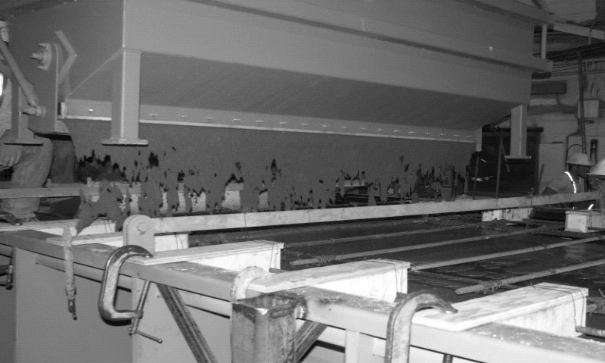
\includegraphics[max width=\textwidth]{moldagem.png}
	\end{center}
	\fonte{\citeonline[p.~17]{Rouse}}
\end{figure}

\begin{figure}[htb]
	\caption{\label{vapor}Cura térmica a vapor.}
	\begin{center}
		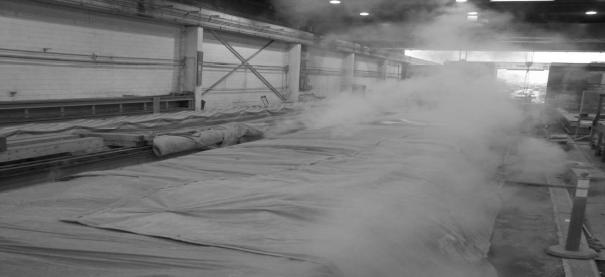
\includegraphics[max width=\textwidth]{vapor.png}
	\end{center}
	\fonte{\citeonline[p.~18]{Rouse}}
\end{figure}

\begin{figure}[htb]
	\caption{\label{corte}Vista em corte.}
	\begin{center}
		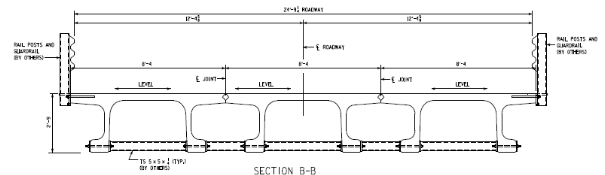
\includegraphics[max width=\textwidth]{corte.png}
	\end{center}
	\fonte{\apudonline[p.~16]{Kei}{Rouse}}
\end{figure}

\begin{figure}[htb]
	\caption{\label{detalhe-juntas}Detalhamento das juntas longitudinais da seção $ \pi $.}
	\begin{center}
		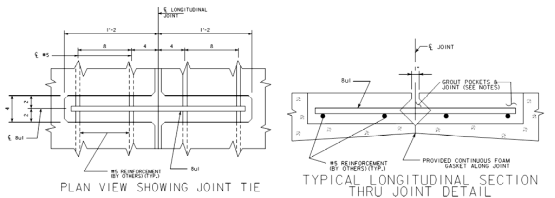
\includegraphics[max width=\textwidth]{detalhe-juntas.png}
	\end{center}
	\fonte{\citeonline[p.~15]{Rouse}}
\end{figure}

\begin{figure}[htb]
	\caption{\label{grauteamento}Grauteamento das juntas longitudinais.}
	\begin{center}
		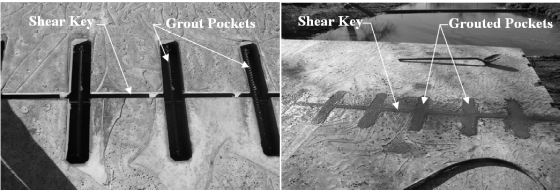
\includegraphics[max width=\textwidth]{grauteamento.png}
	\end{center}
	\fonte{\citeonline[p.~15]{Rouse}}
\end{figure}

\begin{figure}[htb]
	\caption{\label{protensao}Detalhe da protensão.}
	\begin{center}
		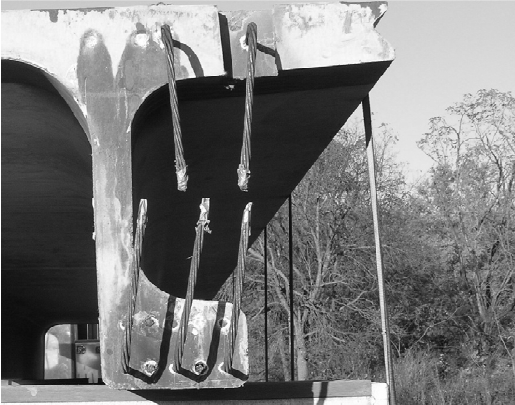
\includegraphics[max width=\textwidth]{protensao.png}
	\end{center}
	\fonte{\citeonline[p.~16]{Rouse}}
\end{figure}

% % %

\begin{figure}[htb]
	\caption{\label{detalhe-diafragma}Detalhamento do diafragma.}
	\begin{center}
		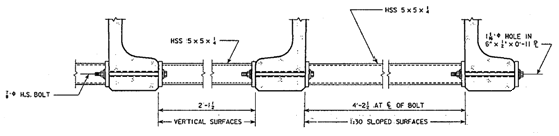
\includegraphics[max width=\textwidth]{detalhe-diafragma}
	\end{center}
	\fonte{\citeonline[p.~14]{Rouse}}
\end{figure}

\begin{figure}[htb]
	\caption{\label{foto-diafragma}Diafragma instalado entre as vigas de uma mesma seção e entre as vigas de seções adjacentes.}
	\begin{center}
		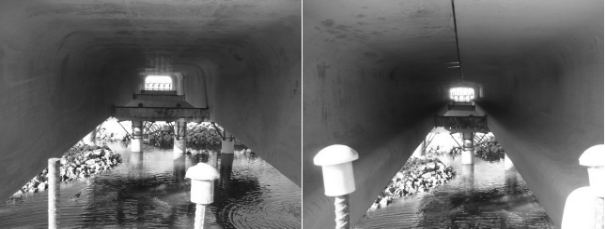
\includegraphics[max width=\textwidth]{foto-diafragma.png}
	\end{center}
	\fonte{\citeonline[p.~14]{Rouse}}
\end{figure}

\begin{figure}[htb]
	\caption{\label{instalacao}Instalação dos elementos estruturais.}
	\begin{center}
		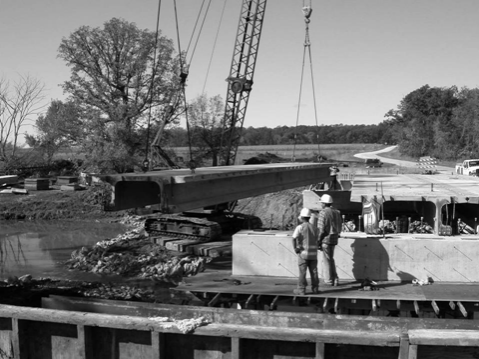
\includegraphics[max width=\textwidth]{instalacao.png}
	\end{center}
	\fonte{\citeonline[p.~18]{Rouse}}
\end{figure}

\begin{figure}[htb]
	\caption{\label{jakway-park}Ponte Jakway Park. Apenas o trecho do vão central é feito de CUAD.}
	\begin{center}
		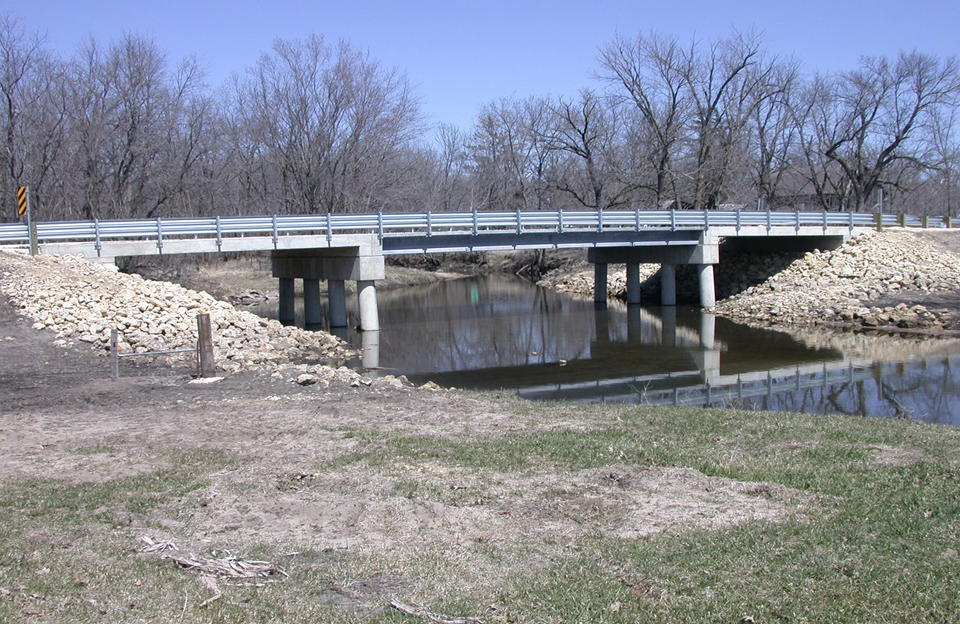
\includegraphics[max width=\textwidth]{jakway-park.png}
	\end{center}
	\fonte{\citeonline{Keierleber_email}}
\end{figure}

%2nd preceedings 579 Design of First Hybrid UHPC-Steel Bridge across the River
%Fulda in Kassel, Germany
\chapter{Esbeltez de uma viga em relação à resistência característica do concreto}

Diante das vantagens apresentada pelo CUAD como solução construtiva, será feita uma análise comparativa acerca da força de protensão necessária para se aplicar em uma viga, a resistência característica do concreto e a área da seção transversal da viga. O objetivo será analisar a economia de material e o vão que poderá ser vencido. Não serão feitas verificações de estado limite último, estado limite de serviço e fissuração. A viga utilizada neste trabalho se baseia no exemplo publicado por \citeonline[p.~37]{Cholfe}.

\nomenclature[A]{ELU}{Estado limite último}
\nomenclature[A]{ELS}{Estado limite de serviço}

\section{Características}

Neste trabalho, será analisada uma viga de seção T com as características mostradas na \autoref{vigat}.

\begin{figure}[htb]
	\caption{\label{vigat} Detalhes da viga de seção  utilizada no estudo de caso.}
		\begin{center}
			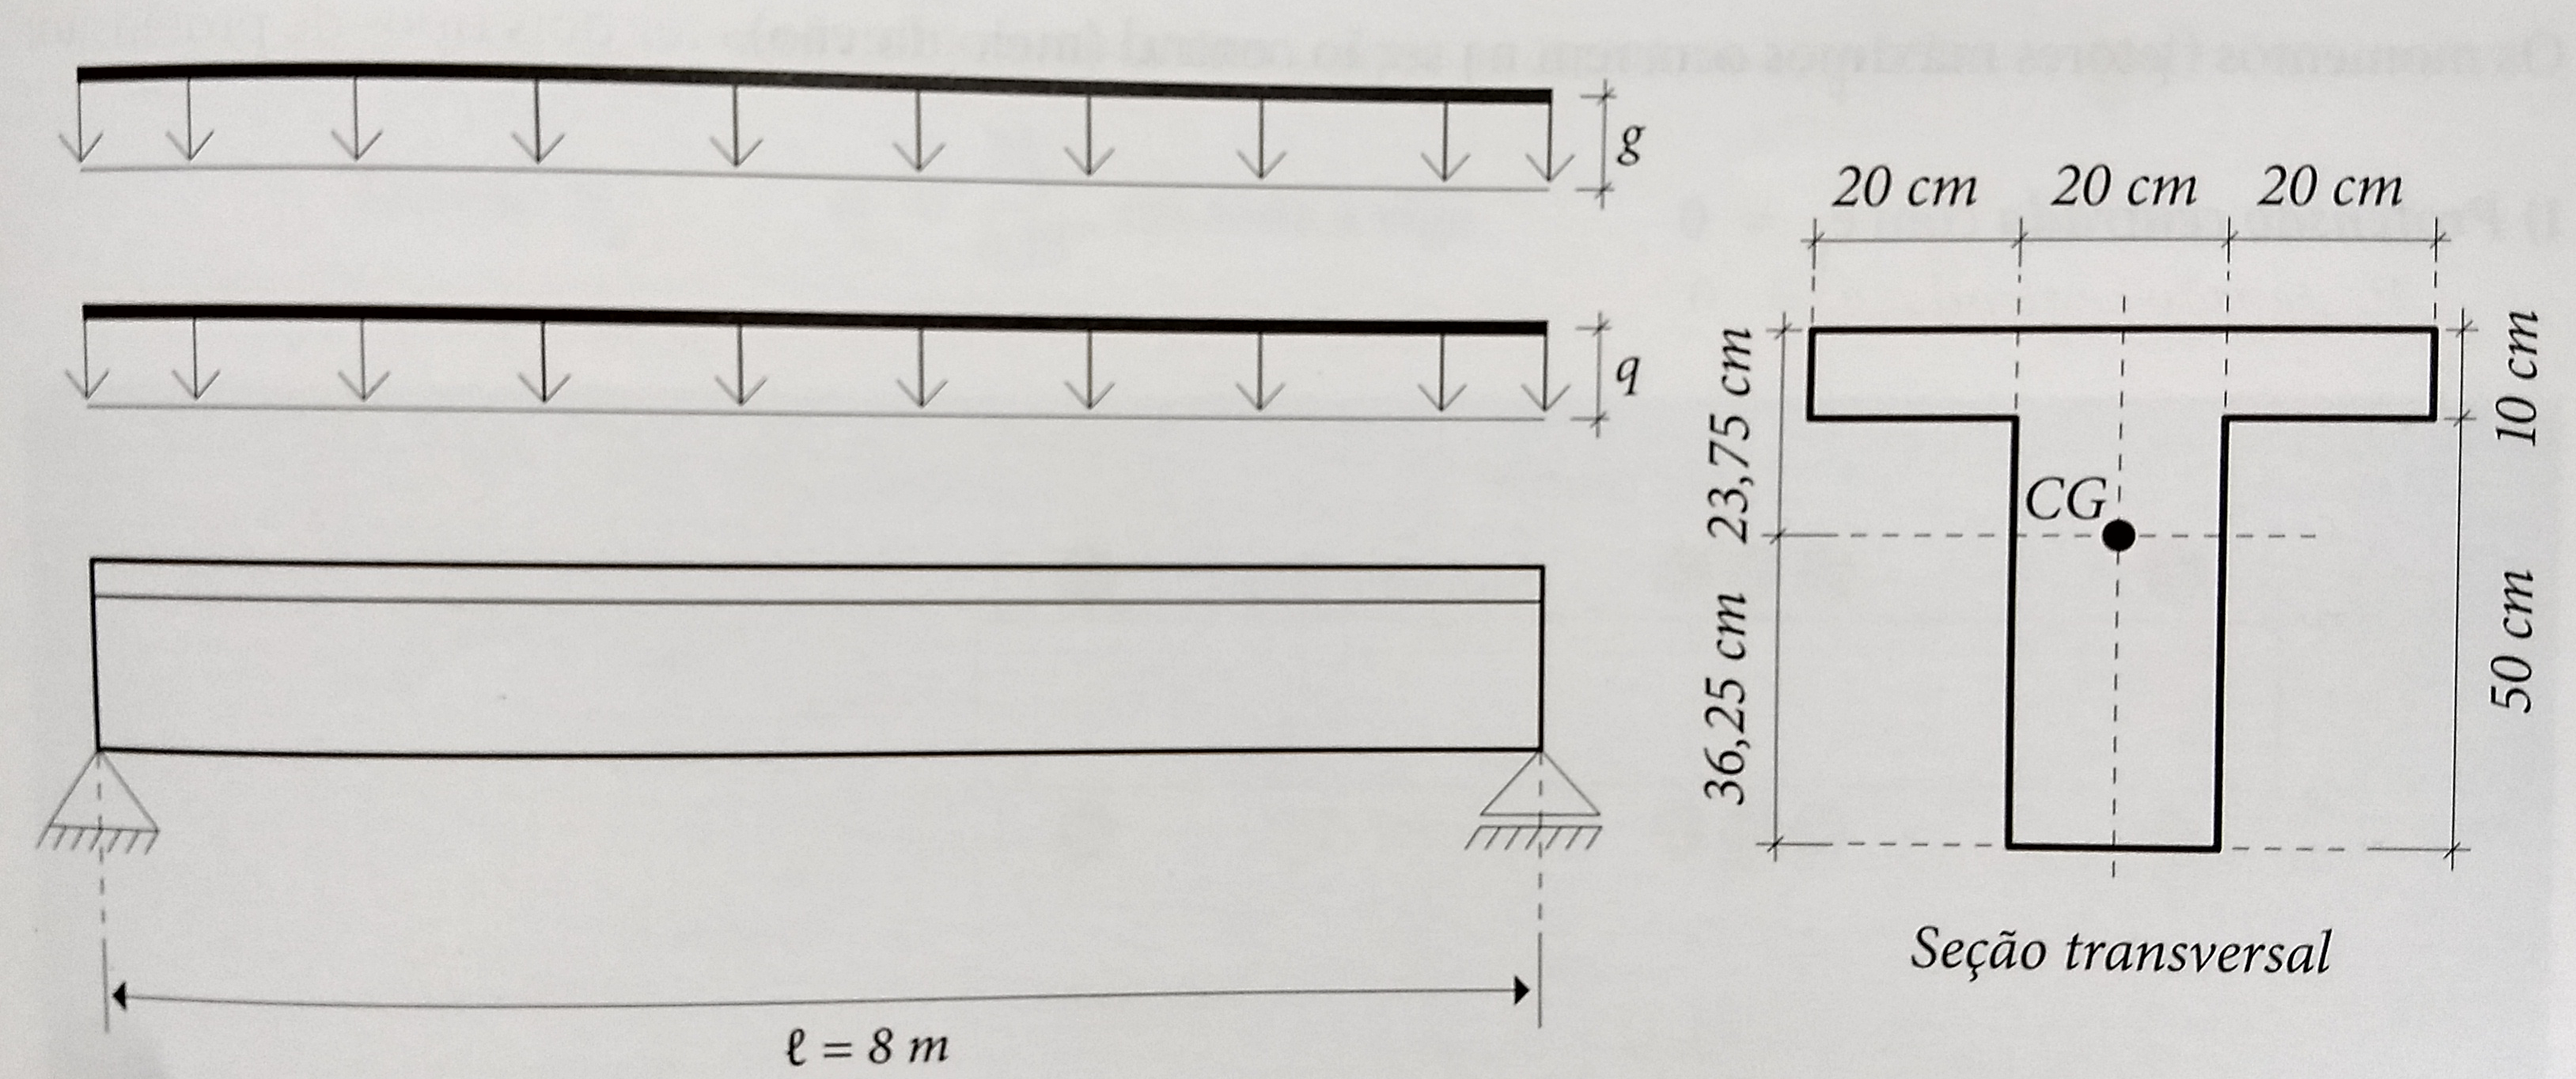
\includegraphics[max width=\textwidth]{viga-t.jpg}
		\end{center}
		\fonte{\citeonline[p.~37]{Cholfe}.}
\end{figure}


O valor da força de protensão será dimensionado considerando o cabo reto e a excentricidade da protensão ($ \text{e}_{\text{p}} $) igual a zero.

\section{Condições de cálculo}

O cálculo das características geométricas da seção, esforços solicitantes e tensões normais foram feitas com o programa de código aberto Scilab. O algoritmo utilizado pode ser visto no \autoref{script}. As condições limites utilizadas são:

\begin{alineas}
	\item Não serão permitidas tensões de tração;
	\item Compressão máxima no concreto: $ 0,6 \cdot \text{fck} $.
\end{alineas}

A viga estará submetida às seguintes ações:

\begin{alineas}
	\item Ação permanente (g): 15 kN/m;
	\item Ação variável (q): 12 kN/m.
\end{alineas}

O cálculo das características geométricas da seção da viga é efetuado pelo programa a partir da entrada de sua altura e largura. É importante notar que o programa desenvolvido para este estudo de caso pode efetuar os cálculos utilizando seções retangulares ou seções T (no caso das seções retangulares, basta que a largura e a espessura da mesa da viga sejam iguais a zero). São calculados apenas os esforços solicitantes característicos (momentos máximos e normal de protensão). O momento máximo permanente ($ \text{M}_{\text{g},\text{max}} $) e variável ($ \text{M}_{\text{q},\text{max}} $) é calculado conforme a \autoref{momento}.

\begin{equation}
	\label{momento}
	\text{M}_{\text{max}} = \text{c} \cdot \frac{\text{l}^2}{8}
\end{equation}

Onde:

\begin{alineas}[label=\textbullet]
	\item c = ação - permanente ou variável (kN/m);
	\item l = vão teórico (m).
\end{alineas}

A tensão permanente ($ \sigma_{\text{c,g,sup}} $) e variável ($ \sigma_{\text{c,q,sup}} $)  na borda superior da viga é calculada conforme a \autoref{tensao_sup} e a tensão permanente ($ \sigma_{\text{c,g,inf}} $) e variável ($ \sigma_{\text{c,q,inf}} $) na borda inferior da viga é calculada conforme a \autoref{tensao_inf}.

\begin{equation}
	\label{tensao_sup}
	\sigma_{\text{c,sup}} = \frac{\text{M}_\text{max}}{\text{W}_\text{sup}}
\end{equation}

Onde:

\begin{alineas}[label=\textbullet]
	\item $ \text{M}_\text{max} $ = momento máximo (kNm);
	\item $ \text{W}_\text{sup} $ = módulo de resistência à compressão superior.
\end{alineas}

\begin{equation}
	\label{tensao_inf}
	\sigma_{\text{c,inf}} = \frac{\text{M}_\text{max}}{\text{W}_\text{inf}}
\end{equation}

Onde:

\begin{alineas}[label=\textbullet]
	\item $ \text{M}_\text{max} $ = momento máximo {kNm};
	\item $ \text{W}_\text{inf} $ = módulo de resistência à compressão inferior.
\end{alineas}

Por convenção, as tensões na borda superior são \textbf{negativas} e as tensões na borda inferior são \textbf{positivas}.

A força normal de protensão é calculada conforme a \autoref{normal}.

\begin{equation}
	\label{normal}
	\text{N}_\text{p} = - \sigma_{\text{c,g,inf}} - \sigma_{\text{c,q,inf}}
\end{equation}

Onde:

\begin{alineas}[label=\textbullet]
	\item $ \sigma_{\text{c,g,inf}} $ = tensão permanente na borda inferior;
	\item $ \sigma_{\text{c,q,inf}} $ = tensão variável na borda inferior.
\end{alineas}

\begin{equation}
	\label{superior}
	\sigma_{\text{c,min,sup}} = \text{N}_\text{p} + \sigma_{\text{c,g,sup}} + \sigma_{\text{c,q,sup}}
\end{equation}

Onde:

\begin{alineas}[label=\textbullet]
	\item $ \text{N}_\text{p} $ = normal de protensão;
	\item $ \sigma_{\text{c,g,sup}} $ = tensão permanente na borda superior;
	\item $ \sigma_{\text{c,q,sup}} $ = tensão variável na borda superior.
\end{alineas}

Após calcular estes parâmetros, o programa faz duas verificações antes de prosseguir com a execução: avalia se a tensão na fibra superior e a força normal de protensão são menores que a compressão máxima permitida (0,6 $\cdot$ fck). A tensão na fibra superior é calculada conforme a \autoref{superior}.


A partir deste ponto, o programa passa a fazer iterações, aumentando o valor do vão teórico de 0,5 m em 0,5 m, até que a protensão aplicada na viga seja pelo menos igual ou maior que 90\% da compressão máxima permitida. Na segunda parte do estudo de caso, a partir de um vão teórico fixo e uma seção transversal inicial, são feitas algumas iterações, em que, no começo de cada iteração, a seção transversal da viga é aumentada em 5\%.  O resultado é mostrado quando atinge-se uma seção transversal em que a viga atende aos critérios estabelecidos (tensão na fibra superior e força normal de protensão menores que a compressão máxima  permitida).

\section{Aplicação}

Com os parâmetros de entrada no algoritmo já definidos, foi gerada a \autoref{tabelafck}, onde pode se observar o crescimento do vão teórico que a viga pode vencer ao se aumentar o fck do concreto e a força de protensão aplicada, ainda atendendo as condições limite definidas e sem alterar a sua seção transversal. O  gráfico da \autoref{graficofck} mostra a relação entre o aumento do fck e o vão que uma mesma viga pode vencer.

É importante notar que a rigidez de uma viga feita com CUAD tende a ser maior que a de uma viga feita com concreto convencional, devido ao seu módulo de elasticidade maior: 50 GPa (valor preliminar que pode ser considerado sem testes, conforme as recomendações da AFGC), mas que pode chegar a 70 GPa, por conta das fibras adicionadas, contra um módulo de elasticidade de 56 GPa na condição mais favorável (agregados de basalto e diabásio) para concretos com de até $ \text{fck} = 90 \quad \text{MPa}  $. Ainda assim, uma peça estrutural muito esbelta sobre um vão muito grande pode gerar deformações e fissuras excessivas. As recomendações da \citeonline{AFGC} contém as instruções necessárias para fazer estas verificações no CUAD.

\begin{figure}[htb]
	\caption{\label{graficofck} Relação do aumento do vão teórico (l) a ser vencido em relação ao aumento do fck}
	\begin{center}
		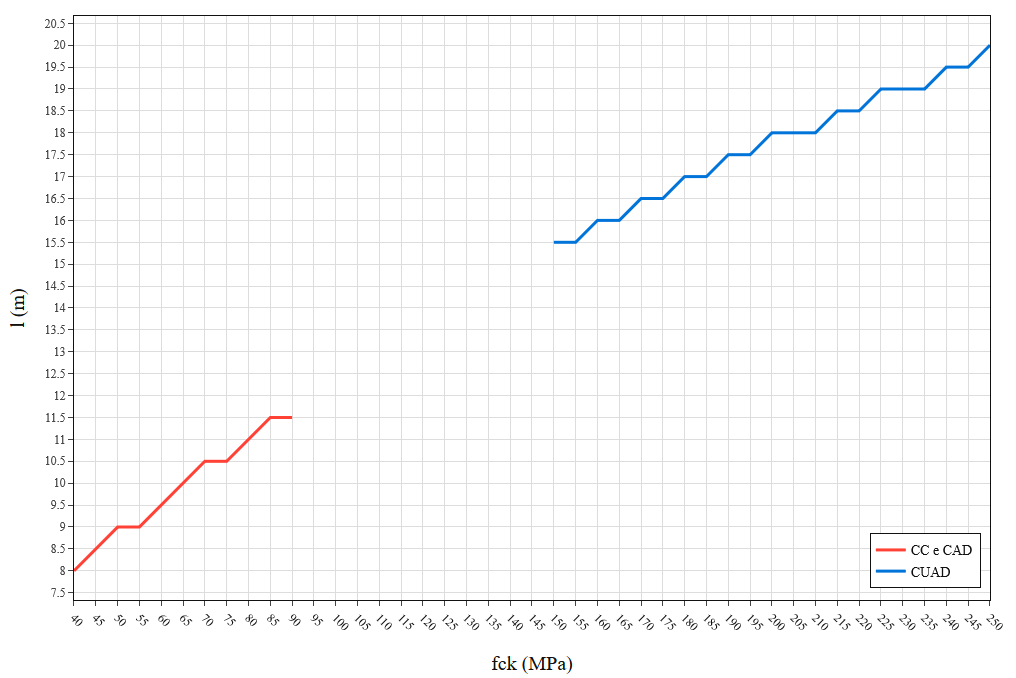
\includegraphics[max width=\textwidth]{Plot4.png}
	\end{center}
%	\fonte{Os autores.}
\end{figure}

%E importante notar que a utilização de seções reduzidas em vigas para vencer grandes vãos pode ser problemática do ponte de vista das deformação da peça. Com $ fck = 40 \text{MPa}$, a rigidez da viga estudada é igual $ kN \cdot m^2 $. Conforme o $ fck $ e o vão teórico aumentam, enquanto a seção transversal

\begin{table}[H]
	\IBGEtab{%
		\caption{Aumento do fck relacionado ao aumento do vão que a mesma viga pode vencer}
		\label{tabelafck}
	}{%
	\begin{tabulary}{\linewidth}{CCCCC}
		\toprule
		fck do concreto (MPa)	&	Protensão máxima (MPa)	&	Protensão necessária $ \sigma_{c,min} $ (MPa)	&	Aproveitamento da protensão máxima (\%)	&	Vão teórico (m)	\\ \midrule  \midrule
		40,00	&	24,00	&	23,53	&	98,03	&	8,00	\\ \midrule
		45,00	&	27,00	&	26,56	&	98,37	&	8,50	\\ \midrule
		50,00	&	30,00	&	29,78	&	99,26	&	9,00	\\ \midrule
		55,00	&	33,00	&	29,78	&	90,24	&	9,00	\\ \midrule
		60,00	&	36,00	&	33,18	&	92,16	&	9,50	\\ \midrule
		65,00	&	39,00	&	36,76	&	94,26	&	10,00	\\ \midrule
		70,00	&	42,00	&	40,53	&	96,50	&	10,50	\\ \midrule
		75,00	&	45,00	&	40,53	&	90,07	&	10,50	\\ \midrule
		80,00	&	48,00	&	44,48	&	92,67	&	11,00	\\ \midrule
		85,00	&	51,00	&	48,62	&	95,33	&	11,50	\\ \midrule
		90,00	&	54,00	&	48,62	&	90,03	&	11,50	\\ \midrule
		
		150,00	&	90,00	&	88,32	&	98,14	&	15,50	\\ \midrule
		155,00	&	93,00	&	88,32	&	94,97	&	15,50	\\ \midrule
		160,00	&	96,00	&	94,11	&	98,03	&	16,00	\\ \midrule
		165,00	&	99,00	&	94,11	&	95,06	&	16,00	\\ \midrule
		170,00	&	102,00	&	100,09	&	98,12	&	16,50	\\ \midrule
		175,00	&	105,00	&	100,09	&	95,32	&	16,50	\\ \midrule
		180,00	&	108,00	&	106,24	&	98,37	&	17,00	\\ \midrule
		185,00	&	111,00	&	106,24	&	95,71	&	17,00	\\ \midrule
		190,00	&	114,00	&	112,59	&	98,76	&	17,50	\\ \midrule
		195,00	&	117,00	&	112,59	&	96,23	&	17,50	\\ \midrule
		200,00	&	120,00	&	119,11	&	99,26	&	18,00	\\ \midrule
		205,00	&	123,00	&	119,11	&	96,84	&	18,00	\\ \midrule
		210,00	&	126,00	&	119,11	&	94,53	&	18,00	\\ \midrule
		215,00	&	129,00	&	125,82	&	97,53	&	18,50	\\ \midrule
		220,00	&	132,00	&	125,82	&	95,32	&	18,50	\\ \midrule
		225,00	&	135,00	&	132,71	&	98,31	&	19,00	\\ \midrule
		230,00	&	138,00	&	132,71	&	96,17	&	19,00	\\ \midrule
		235,00	&	141,00	&	132,71	&	94,12	&	19,00	\\ \midrule
		240,00	&	144,00	&	139,79	&	97,08	&	19,50	\\ \midrule
		245,00	&	147,00	&	139,79	&	95,09	&	19,50	\\ \midrule
		250,00	&	150,00	&	147,05	&	98,03	&	20,00	\\
		
		\bottomrule
	\end{tabulary}%
}{%
%\fonte{Os autores.}%
%\nota{Recomenda-se o uso de água de amassamento de baixa temperatura, pré cura térmica de 2 dias e cura térmica de 24 horas a uma temperatura de 80\textsuperscript{\degree} C.}
%\nota[Anotações]{Uma anotação adicional, que pode ser seguida de várias outras.}
}
\end{table}

\newpage

Em seguida, comparou-se o quanto a seção da viga T feita com concreto de fck igual a 40 MPa até 90 MPa precisaria aumentar para vencer o mesmo vão de uma viga com as mesmas caraterísticas feitas com um CUAD de fck igual a 150 MPa. Pode-se observar um considerável aumento na área da seção transversal, em comparação com os 0,16 $ \text{m}^2 $ da viga de CUAD. A partir dos resultados mostrados na \autoref{comparacao-cuad-cad}, é possível concluir que as seções de vigas feitas  em CUAD são, aproximadamente, 50\% menores que as feitas de concreto convencional (CC) e concreto de alto desempenho (CAD).

\nomenclature[A]{CC}{Concreto convencional}

\begin{table}[htb]
	\IBGEtab{%
		\caption{Aumento da área da seção transversal}
		\label{comparacao-cuad-cad}
	}{%
	\begin{tabulary}{\linewidth}{CCCCCCC}
		\toprule
		fck (MPa)	&	Área da seção ($\text{m}^2$)	&	Taxa de aumento (\%)	\\ \midrule  \midrule
		40	&	0,453	&	64,64	\\ \midrule
		45	&	0,453	&	64,64	\\ \midrule
		50	&	0,360	&	55,56	\\ \midrule
		55	&	0,338	&	52,59	\\ \midrule
		60	&	0,338	&	52,59	\\ \midrule
		65	&	0,338	&	52,59	\\ \midrule
		70	&	0,338	&	52,59	\\ \midrule
		75	&	0,315	&	49,21	\\ \midrule
		80	&	0,315	&	49,21	\\ \midrule
		85	&	0,263	&	39,05	\\ \midrule
		90	&	0,263	&	39,05	\\ \midrule \midrule
			& \textbf{Média} &	51,91	\\
		\bottomrule
	\end{tabulary}%
}{%
%\fonte{Os autores.}%
%\nota{Recomenda-se o uso de água de amassamento de baixa temperatura, pré cura térmica de 2 dias e cura térmica de 24 horas a uma temperatura de 80\textsuperscript{\degree} C.}
%\nota[Anotações]{Uma anotação adicional, que pode ser seguida de várias outras.}
}
\end{table}



%A partir da análise do gráfico, com o auxílio do Excel, propõe-se a equação \autoref{escolha}, para se ter uma ferramenta fácil para escolher o $ fck $ do concreto para uma viga protendida em relação ao vão teórico a ser vencido.
%
%\begin{equation}
%fck = 0,25 \cdot l^2 + 0,4 \cdot l + 21
%\end{equation}
%
%Onde: 
%
%\begin{alineas}[label=\textbullet]
%	\item $ fck $ = resistência característica do concreto aos 28 dias de idade;
%	\item $ l $ = vão teórico a ser vencido.
%\end{alineas}

\chapter{Análise dos resultados}

O processo de pesquisa que resultou na realização deste trabalho permitiu as seguintes análises:

\begin{alineas}[label=\textbullet]
	\item Demonstrou-se a possibilidade da realização de empreendimentos e obras de arte no Brasil em CUAD, a partir dos fundamentos teóricos encontrados na literatura científica nacional e internacional, apesar de ainda não existir uma normatização de seu uso;
	\item Foi possível conhecer as características físicas do CUAD, a partir das quais é possível construir modelos computacionais que permitem a análise de estruturas feitas com o material;
	\item Compreender os benefícios do CUAD como solução construtiva em relação ao concreto convencional, CAD e aço, principalmente nas questões de manutenção da obra (menos manutenção ao longo da vida útil), sustentabilidade ambiental (menor impacto ambiental em seu ciclo de vida produtivo), tempo de execução (que é menor, por conta de seu processo de produção industrializado) e custos (que, apesar de ser maior no início, pode ser compensado ao longo da vida útil da construção, em sua manutenção e durabilidade);
	\item Foi possível conhecer, na revisão bibliográfica, as principais linhas de pesquisa que regem o desenvolvimento do CUAD nos principais centros de pesquisa do mundo, as marcas comerciais já disponíveis no mercado e outras variedades que estão sendo estudados e ainda não são vendidas;
	\item Foi possível conhecer as técnicas utilizadas na execução de estruturas em CUAD, principalmente na questão da distribuição das fibras no concreto e um método utilizado durante a mistura do CUAD utilizado para construir a ponte Jakway Park;
	\item Foi possível fazer um programa que possa auxiliar na análise da viabilidade da aplicação de CUAD em vigas protendidas, auxiliando o engenheiro a entender, com rapidez, a viabilidade da aplicação do material na obra;
	\item No estudo de caso, foi demonstrado que o uso de CUAD na construção de vigas protendidas pode diminuir a sua seção transversal em aproximadamente 50\%;
	\item No estudo de caso, comprovou-se a capacidade do CUAD de permitir a realização de empreendimentos com formas muito esbeltas, dada a sua elevada capacidade de resistência e sua qualidade inerente, fato que também se deve à sua produção industrializada.
\end{alineas}
%\chapter{Projeto de uma ponte de concreto armado}

\section{Objetivo}

Projetar a superestrutura de uma ponte apoiada sobre duas vigas de concreto armado. O projeto
terá a mesma largura e comprimento da seção feita com CUAD da ponte Jakway Park, de modo a comparar
as características do projeto de descobrir vantagens e desvantagens acerca da escolha de cada um dos
métodos no estudo de caso.

\section{Escopo}

Normas brasileiras serão utilizadas para este dimensionamento, mas deixando claro as disparida-
des entre as normas brasileira e as normas estadunidenses, afim de tornar a comparação mais transparente.

\section{Fundamentos para um projeto de pontes}

\citeonline[p.~29, tradução nossa]{Troitsky} afirma que um projeto de pontes é um problema complexo
de engenharia, o qual envolve diversos fatores, como o sistema da ponte, materiais, dimensões, fundações,
estética, paisagem local e ambiente.

Na fase preliminar, o projetista analisa todos os fatores baseado em sua própria criatividade,
experiência, conhecimento e capacidade de inovação (a parte artística do projeto). Em seguida, ocorre o
refinamento do projeto de acordo com os aspectos econômicos e práticos que a obra exige. Depois que
todas as exigências estéticas e funcionais são definidas, parte-se para a fase final do projeto, que requer
um estudo e análise detalhada da estabilidade da ponte e seu comportamento estrutural \cite[p.~30]{Troitsky}.

Um projeto de pontes envolve uma enorme quantidade de dados e diversos outros fatores, mas
por questões de brevidade, a definição acima é suficiente para o desenvolvimento deste trabalho.

\section{Definição: pontes e obras de arte}

Primeiramente, é preciso deixar claro que pontes e obras de arte são termos intercambiáveis.
Segundo \citeonline[p.~29, tradução nossa]{Troitsky}, a caracterização de pontes como obras de arte se deve à mescla de
arte com embasamento técnico, necessários para sua concepção. Estruturalmente falando, pontes, viadutos
e passarelas possuem processos basicamente idênticos de concepção e construção. \citeonline[p.~1]{Pfeil} as
define da seguinte forma (grifo nosso):

\begin{citacao}
Denomina-se \textbf{ponte} a obra destinada a transposição de obstáculos à continui-
dade do leito normal de uma via, tais como rios, braços de mar, vales profundos,
outras vias, etc. Quando a ponte tem por objetivo a transposição de vales,
outras vias ou obstáculos em geral não constituídos por água é, comumente,
denominada \textbf{viaduto}.
\end{citacao}

A NBR 7188 \cite[p.~1, grifo do autor]{NBR7188:2013} dá a seguinte definição:

\begin{citacao}
\textbf{ponte}\\
estrutura sujeita a ação de carga em movimento com posicionamento variável,
aqui chamada de carga móvel, utilizada para transpor obstáculo natural (rio,
córrego, vale, etc.)

[...]\\
\textbf{viaduto}\\
estrutura para transpor obstáculo artificial (avenida, rodovia, etc.)

[...]\\
\textbf{passarela}\\
estrutura longilínea, destinada a transpor obstáculos naturais e/ou artificiais
exclusivamente para pedestres e/ou ciclistas.
\end{citacao}

\nomenclature[A]{OAC}{Obras de arte correntes}
\nomenclature[A]{OAE}{Obras de arte especiais}

Estas obras de arte ainda podem ser divididas em duas categorias: obras de arte correntes (OAC)
e obras de arte especiais (OAE). OAC são construções que possuem um projeto padrão, enquanto OAE
são construções cujo projeto é específico para cada caso \cite{Franca}.

\subsection{Classificação de pontes}

A depender dos critérios do observador, uma ponte pode ser classificada de diferentes maneiras \cite[p.~3]{Pfeil}. Neste trabalho essas obras de arte foram classificadas conforme a natureza do tráfego,
que pode ser rodoviária, ferroviária e rodoferroviária, além das que se destinam apenas para pedestres: as
passarelas.

\subsection{Elementos constituintes}

\citeonline[p.~1]{Pfeil} divide a ponte em três partes principais:

\begin{alineas}[label=\textbullet]
  \item \textbf{infraestrutura}: trata-se da fundação, o elemento estrutural que transmite ao solo ou rocha os esforços vindos da mesoestrutura;
  \item \textbf{mesoestrutura}: comumente são os pilares, os elementos estruturais que recebem os esforços da superestrutura;
  \item \textbf{superestrutura}: conforme a finalidade da construção, constitui a parte útil, composta de lajes, vigas principais e secundárias.
\end{alineas}

Um ponte ainda pode possuir encontros: elementos estruturais responsáveis por receber o
empuxo de aterros de acesso, evitando sua transmissão aos outros elementos da ponte. São extremamente
variáveis e não são necessários em todas as obras de arte \cite[p.~1]{Pfeil}

\begin{figure}[htb]
	\caption{\label{elementos}Vista de uma ponte mostrando seus principais elementos constituintes.}
	\begin{center}
	    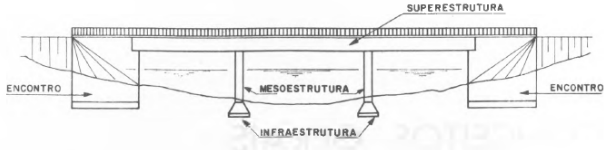
\includegraphics[max width=\textwidth]{elementos.png}
	\end{center}
	\fonte{\citeonline[p.~2]{Pfeil}}
\end{figure}

\subsection{Referências normativas}

\citeonline{DNER}, no Manual de Projeto de Obras de Arte Especiais determina o uso das seguintes normas brasileiras para o desenvolvimento de projetos de pontes (a lista foi atualizada conforme as últimas normas publicadas pela ABNT e NBR 7189, NBR 7197 e a NBR 10839 foram omitidas por terem sido canceladas e/ou substituídas):

\begin{alineas}[label=\textbullet]
  \item NBR 6118:2014 - Projeto de estruturas de concreto - Procedimento;
  \item NBR 7187:2003 - Projeto de pontes de concreto armado e de concreto protendido - Procedimento;
  \item NBR 7188:2013 - Carga móvel rodoviária e de pedestres em pontes, viadutos, passarelas e outras estruturas;
  \item NBR 7190:1997 - Projeto de estruturas de madeira;
  \item NBR 8800:2008 - Projeto de estruturas de aço e de estruturas mistas de aço e concreto de edifícios;
  \item NBR 7191:1982 - Execução de desenhos para obras de concreto simples ou armado;
  \item NBR 6122:2010 - Projeto e execução de fundações;
  \item NBR 6123:1988 - Forças devidas ao vento em edificações;
  \item NBR 6297:1983 - Levantamento geotécnico;
  \item NBR 8681:2003 - Ações e segurança nas estruturas - procedimento;
  \item NBR 9062:2017 - Projeto e execução de estruturas de concreto pré-moldado;
  \item NBR 7480:2007 - Aço destinado a armaduras para estruturas de concreto armado - Especificação;
  \item NBR 7482:2008 - Fios de aço para estruturas de concreto protendido - Especificação;
  \item NBR 7483:2008 - Cordoalhas e aço para estruturas de concreto protendido - Especificação.
\end{alineas}

\subsection{Dados necessários para um projeto de obras de arte}

Muitos dados são necessários para se projetar uma obra de arte. \citeonline[p.~19]{Leonhardt} cita alguns:

\begin{citacao}
1. Planta da situação [...];\\
2. Seção longitudinal [...];\\
3. Largura da ponte [...];\\
4. Condições das fundações [...];\\
5. Condições locais [...];\\
6. Condições meteorológicas e ambientais [...];\\
7. Estética e meio ambiente [...];\\
8. Exigências relativas ao ambiente [...].
\end{citacao}

Também é imprescindível que o projetista visite o local ou pelo menos tenha acesso a fotos de
altíssima qualidade \cite[p.~19]{Leonhardt}.

\subsection{Ações consideradas em pontes}

\nomenclature[A]{ABNT}{Associação Brasileira de Normas Técnicas}

No Brasil, os carregamentos e esforços atuantes utilizados para o projeto de pontes é fixado pela
ABNT (Associação Brasileira de Normas Técnicas). Desse modo, a NBR 7187 \cite[p.~3]{NBR7187:2013} define ações como as causas que provocam o aparecimento de esforços ou deformações nas estruturas e
as divide em três categorias:

\begin{alineas}
  \item  permanentes;
  \item  variáveis;
  \item  excepcionais.
\end{alineas}

\apudonline[p.~36]{Mason}{Hoss} lista as principais ações a que uma ponte é solicitada:

\begin{citacao}
a) Carga permanente. É avaliada com base no peso específico do concreto armado ou protendido, [...], além do peso de outros elementos, tais como pavimentação, guarda-corpos, guarda-rodas, [...];

b) Carga móvel. É fixada de acordo com o tipo de ponte e a classe de rodovia ou ferrovia. [...];

c) Impacto vertical e impacto lateral. As cargas móveis produzem efeitos dinâmicos diversos, em consequência de sua própria mobilidade, irregularidades da pista, etc.;

d) Força longitudinal. A força longitudinal é devida à frenagem e à aceleração dos veículos ou trens sobre as pontes. [...];

e) Força centrífuga. Nas pontes em curva, a carga móvel transmite à ponte uma força centrífuga [...];

f) Vento. Incide transversalmente sobre a ponte e a carga móvel, sendo o seu efeito avaliado através de pressões por unidade de área, [...];

g) Efeitos térmicos, atrito nos apoios, empuxos, movimento das fundações, etc.

Deverão ser considerados, em cada caso, de acordo com as condições especiais
da obra.
\end{citacao}

Este trabalho visa apenas dimensionar a superestrutura da ponte, portanto só serão consideradas as
ações permanentes e móveis. As ações de empuxo, variação de temperatura, vento, frenagem e aceleração
não são levadas em conta ao se lidar com a superestrutura \cite{Andrade}.

\section{Características do concreto a ser utilizado}

\nomenclature[A]{CAA}{Classe de agressividade ambiental}

A NBR 6118 \cite[p.~17]{NBR6118:2014} estabelece o uso de quatro classes de agressividade ambiental
(CAA): fraca, moderada, forte e muito forte. A ponte deste trabalho se encaixa na CAA I, agressividade
fraca e ambiente rural, portanto o risco de deterioração da estrutura é insignificante.

A partir da definição da CAA, a NBR 6118 \cite[p.~18-20	]{NBR6118:2014} determina a relação
água/cimento do concreto a ser utilizado, bem como o cobrimento nominal da armadura. Conforme a
recomendação, esta ponte deverá utilizar um concreto com relação água/cimento $ leq $ 0,65 e f\textsubscript{ck} $ geq $ 20 MPa (concreto classe 20). Para a ponte em questão, o cobrimento nominal da laje (tabuleiro da ponte) deverá ser de 20 mm. este trabalho, opta-se por utilizar um concreto com f\textsubscript{ck} = 30 MPa (concreto classe C30). Estas
definições estão resumidas na \autoref{definicoes}.

\begin{table}[htb]
\IBGEtab{%
  \caption{Definições da construção.}
  \label{definicoes}
}{%
  \begin{tabulary}{\linewidth}{CCCC}
  \toprule
  Classe de agressividade
  ambiental                 & Relação água/cimento & Cobrimento nominal da laje (mm) & Classe do concreto \\
  \midrule \midrule
   I                        & $ \leq $ 0,65        & 20                              & C30   \\
   \bottomrule
\end{tabulary}%
}{%
  \fonte{elaborado pelo autor.}%
  %\nota{Recomenda-se o uso de água de amassamento de baixa temperatura, pré cura térmica de 2 dias e cura térmica de 24 horas a uma temperatura de 80\textsuperscript{\degree} C.}
  %\nota[Anotações]{Uma anotação adicional, que pode ser seguida de várias outras.}
  }
\end{table}

\section{Pré-dimensionamento da laje}

Para estimar a espessura da laje, \citeonline[p.~53]{Leonhardt} recomenda, primeiramente, definir o
seu índice de esbeltez. \citeonline[p.~39]{Pretti} o define como "a distância aproximada entre os pontos de
momento nulo do diagrama de momentos provocado pela carga permanente"dividido pela altura da seção
transversal. Este índice é calculado conforme a \autoref{indice-esbeltez}

\begin{equation}\label{indice-esbeltez}
I_e = \frac{\ell}{h}
\end{equation}

Onde:

$ I_e = $ índice de esbeltez;

$ \ell = $ distância aproximada entre os pontos de momento nulo do diagrama de momentos provocado pela carga permanente;

$ h = $ altura da seção transversal.

\nomenclature[S]{$ I_e $}{Índice de esbeltez}
\nomenclature[S]{$ \ell $}{Distância aproximada entre os pontos de momento nulo do diagrama de momentos provocado pela carga permanente}
\nomenclature[s]{$ h $}{Altura da seção transversal}

Para o projeto em questão, uma ponte de laje maciça bi apoiada, o valor de $ \ell $ coincide com o valor
do vão teórico. \citeonline[p.~54]{Leonhardt} recomenda que o índice de esbeltez de uma ponte de laje maciça
de concreto armado classe 45 deve variar entre 15 e 22. Considerando o índice de esbeltez máximo, a
altura de laje a ser utilizada deve ser igual a 71 cm\footnote{Resolvendo a \autoref{indice-esbeltez} para h:\\ $ h = \frac{\ell}{I_e} \rightarrow h = \frac{15,6}{22} = 0,709 $}.

\section{Ações permanentes}

A NBR 7187 \cite[p.~4]{NBR7187:2013} define ações permanentes como ``Ações cujas intensidades podem ser consideradas como constantes ao longo da vida útil da construção[, incluindo] as que crescem no tempo, tendendo a um valor limite constante''.

\nomenclature[S]{kN/m\textsuperscript{2}}{Quilonewton por metro quadrado}

Além do peso próprio da laje e da pavimentação, a NBR 7187 \cite[p.~4]{NBR7187:2013} determina que deve ser considerada uma carga adicional de 2 kN/m\textsuperscript{2}, para um futuro recapeamento. A \autoref{cargas} resume os carregamentos permanentes distribuídos da ponte.

\nomenclature[S]{kN/m\textsuperscript{2}}{Quilonewton por metro quadrado}
\nomenclature[S]{kN/m\textsuperscript{3}}{Quilonewton por metro cúbico}

\begin{table}[htb]
\IBGEtab{%
  \caption{Peso específico, espessura e carregamentos distribuídos dos elementos da ponte.}
  \label{cargas}
}{%
  \begin{tabulary}{\linewidth}{CCCC}
  \toprule
   Elemento     & Peso específico (kN/m\textsuperscript{3}) & Espessura (m) & Carregamento distribuído (kN/m\textsuperscript{2}) \\
  \midrule \midrule
   Laje         & 25 \textsuperscript{a} & 0,71                    & 17,75 \\ \midrule 
   Pavimentação & 24 \textsuperscript{b} & 0,1 \textsuperscript{c} & 2,40  \\ \midrule 
   Sobrecarga   & -                      & -                       & 2 \textsuperscript{d}     \\ \midrule 
   Total        & -                      & -                       & 22,15 \\
  \bottomrule
\end{tabulary}%
}{%
  \fonte{elaborado pelo autor.}%
  \legend{ \footnotesize
  Notas: \newline
  \textsuperscript{a} Conforme NBR 6118 \cite[p.~22]{NBR6118:2014}. \newline
  \textsuperscript{b} Conforme NBR 7187 \cite[p.~4]{NBR7187:2013}. \newline
  \textsuperscript{c} Conforme Pretti \cite[p.~103]{Pretti}. \newline
  \textsuperscript{d} Conforme NBR 7187 \cite[p.~4]{NBR7187:2013}
  }
  %\nota[Anotações]{Uma anotação adicional, que pode ser seguida de várias outras.}
  }
\end{table}
Para efeito de cálculo, considera-se que a laje é um elemento isotrópico, e suas solicitações são calculadas com a teoria elástica das lajes \citeonline[p.~41]{Pretti}. Neste trabalho, optou-se por utilizar as tabelas publicadas por \citeonline{Rusch}, de modo a se calcular os valores dos momentos fletores e esforços cortantes, já que as normas brasileiras de cargas rodoviárias adotam o mesmo carregamento das normas alemãs, para o qual as tabelas foram feitas. A partir das tabelas, podemos adquirir os maiores valores dos carregamentos em suas posições mais desfavoráveis. Para automatizar o uso das tabelas de cálculo, foi utilizado o programa \textit{freeware} T-Rüsch  \cite{Serapiao_e_Khouri}.

Para calcular os esforços permanentes através das tabelas de Rüsch, além de definir as condições de apoio, é preciso definir os valores das seguintes variáveis:

\begin{alineas}[label=\textbullet]
  \item $ \ell_x $: direção principal da placa (direção dos momentos máximos);
  \item $ \ell_y $: direção ortogonal a $ \ell_x $;
  \item a: espaçamento entre rodas do veículo de cálculo (definido na NBR 7188);
  \item t: largura da distribuição de carga do veículo de cálculo (definido na NBR 7188).
\end{alineas}

\nomenclature[S]{$ \ell_x $}{Direção principal da placa (direção dos momentos máximos)}
\nomenclature[S]{$ \ell_y $}{Direção ortogonal a $ \ell_x $}
\nomenclature[S]{a}{Espaçamento entre rodas do veículo de cálculo}
\nomenclature[S]{t}{Largura da distribuição de carga do veículo de cálculo}
\nomenclature[S]{g}{Carregamento distribuído}

E em seguida determinar as relações $ \nicefrac{\ell_y}{\ell_x} $, $ \nicefrac{\ell_x}{a} $ e $ \nicefrac{t}{a} $. A \autoref{condicoes-apoio} exibe as condições de apoio da laje em questão e a \autoref{dados-rusch} define as variáveis descritas acima.

\begin{figure}[htb]
	\caption{\label{condicoes-apoio}Condições de apoio da laje. A linha cheia informa que a borda é simplesmente apoiada; a tracejada, borda livre.}
	\begin{center}
	    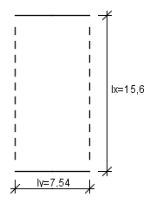
\includegraphics[max width=\textwidth]{condicoes-apoio.png}
	\end{center}
	\fonte{elaborado pelo autor}
\end{figure}

\begin{table}[htb]
\IBGEtab{%
  \caption{Definição das variáveis.}
  \label{dados-rusch}
}{%
  \begin{tabulary}{\linewidth}{CCCCC}
  \toprule
  $ \ell_x $ (m)   & $ \ell_y $ (m) &  a (m)      & t (m)        & Relações \\
  \midrule \midrule
    15,6      &  7,54      &  2      & 0,32 
   &
     $ \ell_x/\ell_y = 0,48 $
     
     $ \ell_x/a = 7,80 $
     
     $ t/a = 0,16 $ \\
  \bottomrule
  \end{tabulary}%
}{%
  \fonte{elaborado pelo autor.}%
  %\nota[Anotações]{Uma anotação adicional, que pode ser seguida de várias outras.}
  }
\end{table}

Se os valores das relações acima não existirem nas tabelas, o valor dos coeficientes é calculado por interpolação linear entre os valores disponíveis na tabela. Neste caso, o T-Rüsch faz isso automaticamente.

Por fim, o cálculo dos carregamentos permanentes é efetuado conforme a \autoref{momento} e a \autoref{cortante} \cite[adaptado]{Rusch}.

\begin{equation} \label{momento}
M = k \cdot g \cdot {\ell_x}^2
\end{equation}

\begin{equation} \label{cortante}
V = k \cdot g \cdot {\ell_x}
\end{equation}

Onde:

$ M = $ momento fletor; \\ \indent
$ V = $ esforço cortante; \\ \indent
$ k = $ coeficiente fornecido nas tabelas de Rüsch; \\ \indent
$ g = $ carregamento distribuído; \\ \indent
$ \ell_x = $ direção principal da placa (direção dos momentos máximos).

\nomenclature[S]{$ M $}{Momento fletor}
\nomenclature[S]{$ V $}{Esforço cortante}
\nomenclature[S]{$ g $}{Carregamento distribuído}
\nomenclature[S]{$ k $}{Coeficiente fornecido nas tabelas de Rüsch}

\subsection{Momentos fletores e esforços cortantes}

A \autoref{momentos-cortantes} exibe os resultados dos momentos fletores e das forças cortantes máximas resultantes das ações permanentes sobre a estrutura.


\begin{table}[htb]
\IBGEtab{%
  \caption{Momentos fletores e esforços cortantes.}
  \label{momentos-cortantes}
}{%
%\begin{tabular*}{\textwidth}{c @{\extracolsep{\fill}} ccccc}
\begin{tabulary}{1.0\textwidth}{CCCCCC}
\toprule
     & k \textsuperscript{*} & g (kN/m$^3 $) & $\ell_x (m)$ &  Resultados \\ \midrule \midrule
M\textsubscript{xm} \textsuperscript{a} & 0,125 \textsuperscript{*} &   &   & 673,80 kNm/m \\ \cmidrule{1-2}\morecmidrules \cmidrule{5-5}
M\textsubscript{ym} \textsuperscript{b} & 0,009 \textsuperscript{*} &        &  & 31,65 kNm/m \\  \cmidrule{1-2}\morecmidrules \cmidrule{5-5}
M\textsubscript{xr} \textsuperscript{c} & 0,125 \textsuperscript{*} & 22,15  & 16,6 & 673,80 kNm/m \\  \cmidrule{1-2}\morecmidrules \cmidrule{5-5}
V\textsubscript{em} \textsuperscript{d} & 0,5 \textsuperscript{**}  &      	 &  & 172,77 kN/m \\  \cmidrule{1-2}\morecmidrules \cmidrule{5-5}
V\textsubscript{er} \textsuperscript{e} & 0,5 \textsuperscript{**}  &        &  & 172,77 kN/m \\
\bottomrule
\end{tabulary} 
}{%
  \fonte{elaborado pelo autor}%
  \legend{ \footnotesize
    Notas: \newline
    \textsuperscript{a} Momento fletor da placa na direção x. \newline
    \textsuperscript{b} Momento fletor no meio da placa na direção y. \newline
    \textsuperscript{c} Momento fletor no meio dos bordos livres da placa na direção x. \newline
    \textsuperscript{d} Força cortante no meio dos apoios. \newline
    \textsuperscript{e} Força cortante no canto dos apoios. \newline
    \textsuperscript{*} Valor extraído da tabela 13 de Rüsch. \newline
    \textsuperscript{**} Valor extraído da tabela 99 de Rüsch. \newline
    \textsuperscript{***} Valor extraído da tabela 101 de Rüsch. \newline
  }
  %\nota[Anotações]{Uma anotação adicional, que pode ser seguida de várias outras.}
  }
\end{table}

\nomenclature[S]{M\textsubscript{xm}}{Momento fletor da placa na direção x}
\nomenclature[S]{M\textsubscript{ym}}{Momento fletor no meio da placa na direção y}
\nomenclature[S]{M\textsubscript{xr}}{Momento fletor no meio dos bordos livres da placa na direção x}
\nomenclature[S]{V\textsubscript{em}}{Força cortante no meio dos apoios}
\nomenclature[S]{V\textsubscript{er}}{Força cortante no canto dos apoios}

Por questões de economia e racionalização, para que se possa detalhar as armaduras, também é necessário calcular os momentos a cada décima parte do vão (neste caso, a cada 1,5 m). O valor do momento em determinada seção x da laje em estudo pode ser definido conforme a \autoref{momentos-secao}.

\begin{equation} \label{momentos-secao}
M_s = V_{max} \cdot x -\frac{g \cdot x^2}{2}
\end{equation}

Onde:

$ M_s = $ momento na seção;

$ V_{max} =  $ esforço cortante máximo;

$ g = $ carregamento distribuído.

Para fins de didáticos e de brevidade, optou-se por ignorar a contribuição de esforços provenientes das barreiras laterais, exigidas para a construção.

\section{Ações variáveis}

A NBR 7187 \cite[p.~5]{NBR7187:2013} define as ações variáveis da seguinte forma:

\begin{citacao}
Ações de caráter transitório, que compreendem, entre outras:

a) as cargas móveis;\\
b) as cargas de construção;\\
c) as cargas de vento;\\
d) o empuxo de terra provocado por cargas móveis;\\
e) a pressão da água em movimento;\\
f) o efeito dinâmico do movimento das águas;\\
g) as variações de temperatura.\\
\end{citacao}

Conforme o escopo deste trabalho, só será calculado o efeito das cargas móveis (veículos que trafegam sobre a via) sobre a laje, de acordo com as orientações da NBR 7188 \cite{NBR7188:2013}.

O cálculo da carga móvel é efetuado conforme a \autoref{carga-movel-concentrada} e a \autoref{carga-movel-distribuida}.

\begin{equation} \label{carga-movel-concentrada}
Q = P \cdot CIV \cdot CNF \cdot CIA
\end{equation}

\begin{equation} \label{carga-movel-distribuida}
q = p \cdot CIV \cdot CNF \cdot CIA
\end{equation}

Onde:

$ Q = $ carga móvel concentrada aplicada no nível do pavimento; \\ \indent
$ q = $ carga móvel estática aplicada no nível do pavimento; \\ \indent
$ P = $ carga estática aplicada no nível do pavimento; \\ \indent
$ CIV = $ coeficiente de impacto vertical; \\ \indent
$ CNF = $ coeficiente de número de faixas; \\ \indent
$ CIA = $ coeficiente de impacto adicional. \\ \indent

\nomenclature[S]{Q}{C	arga móvel concentrada aplicada no nível do pavimento}
\nomenclature[S]{q}{Carga móvel estática aplicada no nível do pavimento}
\nomenclature[S]{P}{Carga estática aplicada no nível do pavimento}
\nomenclature[S]{CIV}{Coeficiente de impacto vertical}
\nomenclature[S]{CNF}{Coeficiente de número de faixas}
\nomenclature[S]{CIA}{Coeficiente de impacto adicional}

Os coeficientes citados acima são calculados conforme a \autoref{CIV}, a \autoref{CNF} e a \autoref{CIA}.

\subsection{Coeficiente de impacto vertical}

\begin{equation} \label{CIV}
  \begin{split}
    CIV = 1,35     & \textrm{ \hspace{2em} para vãos menores que 10,0 m} \\
    CIV = 1 + 1,06 \cdot \frac{20}{Liv + 50} & \textrm{ \hspace{2em} para vãos entre 10,0 m e 200,0 m}
  \end{split}
\end{equation}

Onde:

$ Liv = $ vão da estrutura, em metros; em estruturas em balanço, é o comprimento do próprio balanço; em estruturas de vãos contínuos, é a média aritmética dos vãos.	

\subsection{Coeficiente de número de faixas}

\begin{equation} \label{CNF}
  CNF = 1 0,05 \cdot (n-2) \geq 0,9
\end{equation}

Onde:

$ n = $ número de faixas.

\subsection{Coeficiente de impacto adicional}

\begin{equation} \label{CIA}
  \begin{split}
    CIA = 1,15 & \textrm{ \hspace{2em} para obras em aço} \\
    CIA = 1,25 & \textrm{ \hspace{2em} para obras em concreto ou mistas}
  \end{split}
\end{equation}

\subsection{Carga móvel rodoviária}

A NBR 7188 \cite{NBR7188:2013} define a carga móvel rodoviária da seguinte forma:

\nomenclature[S]{kN}{Quilonewton}
\nomenclature[S]{m\textsuperscript{2}}{Metro quadrado}
\begin{citacao}
A carga móvel rodoviária padrão TB-450 é definida por um veículo tipo de 450 kN, com seis rodas P = 75 kN, três eixos de carga afastados entre si em 1,5 m, com área de ocupação de 18,0 m\textsuperscript{2}, circundada por uma carga uniformemente distribuída constante p = 5 kN/m\textsuperscript{2} [...].
\end{citacao}

A \autoref{disposicao-cargas-estaticas} ilustra o excerto acima.

\begin{figure}[htb]
	\caption{\label{disposicao-cargas-estaticas}Disposição das cargas estáticas.}
	\begin{center}
	    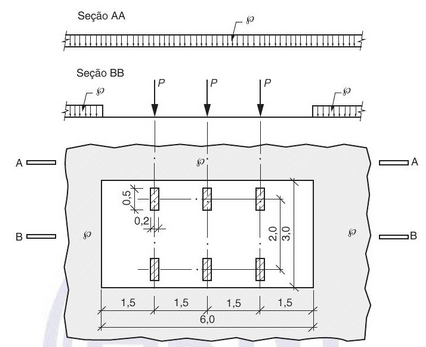
\includegraphics[max width=\textwidth]{disposicao-cargas-estaticas.png}
	\end{center}
	\fonte{NBR 7188 \cite{NBR7188:2013}}
\end{figure}

\subsection{Momentos resultantes}

Os momentos resultantes\footnote{Veja a \autoref{momentos-cortantes} para ver a qual momento cada item dos resultados se refere.} das cargas acidentais obtidos a partir do T-Rüsch são:

\nomenclature[S]{kNm/m}{Quilonewton metro por metro}

$ M_{xm} = $ 80,38 kNm/m \\ \indent
$ M_{ym} = $ 453,53 kNm/m \\ \indent
$ M_{yr} = $ 503,66 kNm/m

O memorial de cálculo gerado pelo programa T-Rüsch pode ser encontrado no \autoref{chap:memorial}

% Finaliza a parte no bookmark do PDF
% para que se inicie o bookmark na raiz
% e adiciona espaço de parte no Sumário
% ----------------------------------------------------------
\phantompart

% ---
% Conclusão
% ---
\chapter{Considerações finais}
% ---

Ao finalizar-se esta pesquisa sobre concreto de ultra alto desempenho, o desenvolvimento do algoritmo para analisar a viabilidade de aplicação do CUAD em vigas de retangular e seção T, é possível afirmar que atingiu-se os objetivos aos quais este estudo se propôs, a saber: uma pesquisa inédita sobre o CUAD como material, seu processo de execução, as considerações efetuadas na modelagem computacional, verificação da capacidade técnica da indústria nacional de produzir os insumos necessários para a fabricação de CUAD no Brasil e desenvolver um método simples para que o projetista possa considerar a aplicação de CUAD nas vigas do seu empreendimento.

Com base em critérios de análise e projeto, é possível concluir que o CUAD é uma solução viável em vários tipos de situações, desde arquitetônicas a estruturais, vide as diversas construções já realizadas pelo mundo, trazendo a possibilidade de se construir estruturas mais esbeltas, resistentes e duráveis. Para que suas propriedades sejam utilizadas ao máximo, é preciso quantificar todos as informações associadas ao projeto, para que se possa chegar a uma solução viável técnica e economicamente. O CUAD proporciona uma maior vida útil da construção a um custo menor de manutenção, o que pode viabilizar o seu uso em diversos empreendimentos, apesar do seu maior custo inicial em relação a outras soluções construtivas.

Também é possível concluir que ainda existe um grande espaço para se desenvolver soluções inovadoras, tanto em geometria como em topologia das peças estruturais utilizadas na construção civil com CUAD, por conta das características de resistência e durabilidade inerentes do material. Ainda, por conta de seu processo industrializado de fabricação, também pode-se concluir que isso trará uma melhora de qualidade na indústria da construção do país.


\chapter{Recomendações para trabalhos futuros}

O algoritmo apresentado neste trabalho (\autoref{script}) faz uma verificação muito simples para analisar a viabilidade da aplicação de CUAD em vigas de seção retangular e seção T. Sugere-se a expansão do método utilizado neste trabalho, afim de se considerar verificações como fissuração da peça, estado limite último (ELU) e estado limite de serviço (ELS), além de se considerar outras peças estruturais (lajes e pilares). Como já foi demonstrado no estudo de caso, o algoritmo provou-se uma maneira útil e prática para a tarefa a qual se destina.


% ----------------------------------------------------------
% ELEMENTOS PÓS-TEXTUAIS
% ----------------------------------------------------------
\postextual
% ----------------------------------------------------------

% ----------------------------------------------------------
% Referências bibliográficas
% ----------------------------------------------------------
\bibliography{referencias-bibliograficas}

% ----------------------------------------------------------
% Glossário
% ----------------------------------------------------------
%
% Consulte o manual da classe abntex2 para orientações sobre o glossário.
%
%\glossary

% ----------------------------------------------------------
% Apêndices
% ----------------------------------------------------------

% ---
% Inicia os apêndices
% ---
\begin{apendicesenv}

\partapendices

\chapter{Algoritmo utilizado no estudo de caso}
\label{script}

Este algoritmo foi utilizado no Scilab 6.0.0 (http://scilab.org) e está disponível sob a licença GNU GPL V2.

%\lstset{\basicstyle=\ttfamily,\breaklines=true}
%\lstinputlisting{apendices/main.sce}
\begin{lstlisting}
/*
 * Author: Douglas Araujo de Moura (douglas.moura [at] constrinew.com.br)
 * Author URI: https://engenharialivre.com/
 * License: GNU General Public License v2 or later
 * License URI: http://www.gnu.org/licenses/gpl-2.0.html
 * Last modified: 2017-11-14
*/

function x = resultados(b, h, bf, hf, g, q, l, fck)
    compressao_maxima = 0.6 * fck * 1000

    [Ac, I, Wsup, Winf] = caractGeometricas(b, h, bf, hf)
    [Mgmax, Mqmax, sigma_cg_inf, sigma_cg_sup, sigma_cq_inf, sigma_cq_sup, Npd] = esforcosSolicitantes(g, q, l, Wsup, Winf)

    Np = ( - sigma_cg_inf - sigma_cq_inf ) * Ac

    sigma_c_min = Npd + sigma_cg_sup + sigma_cq_sup

    if abs(sigma_c_min) < abs(compressao_maxima) then
        v1 = 1
    else
        v1 = 0
        //warning("A tensão na fibra superior (|" + string(sigma_c_min/1000)  + "| MPa) é maior que a máxima permitida (|" + string(compressao_maxima/1000)  + "| MPa).")
    end

    if abs(Npd) < abs(compressao_maxima) then
        v2 = 1
    else
        v2 = 0
        //warning("A compressão na seção dos apoios (|" + string(Npd/1000)  + "| MPa) é maior que a máxima permitida (|" + string(compressao_maxima/1000)  + "| MPa).")
    end

    // 1. Normal de protensão (MPa)
    // 2. fck do concreto (MPa)
    // 3. Compressão máxima permitida (MPa)
    // 4. Compressão mínima no concreto (MPa)
    // 5. Taxa de aproveitamento da compressão no concreto (%)
    // 6. Vão teórico (m)
    // 7. Status da primeira validação (boolean)
    // 8. Status da segunda validação (boolean)
    // 9. Área da seção transversal
    // 10. Inércia da seção
    // 11. W_sup
    // 12. W_inf
    x = [(Npd/1000) fck (abs(compressao_maxima)/1000) ((abs(sigma_c_min))/1000) ((abs(sigma_c_min) / abs(compressao_maxima)) * 100) l v1 v2 Ac I Wsup Winf]

endfunction

function [Ac, I, Wsup, Winf] = caractGeometricas(b, h, bf, hf)
    if bf == 0 & hf == 0 then
        // Seção retangular
        Ac = b * h
        I  = (b * (h^3)) / 12
        y = h / 2
        Wsup = I / y
        Winf = I / y
    else
        // Seção T
        h     = (h - hf)
        A1    = bf * hf
        A2    = b  * h
        Ac    = A1 + A2
        Msx   = (A1 * (h + (hf / 2))) + (A2 * (h / 2))
        yg    = Msx / Ac
        I_xg1 = ((bf * (hf^3)) / 12) + (bf * hf * (((h + (hf / 2)) - yg)^2))
        I_xg2 = ((b * (h^3)) / 12) + (b * h * ((yg - (h / 2))^2))
        I     = I_xg1 + I_xg2
        ysup  = (h + hf) - yg
        yinf  = yg
        Wsup  = I / ysup
        Winf  = I / yinf
    end
endfunction

function [Mgmax, Mqmax, sigma_cg_inf, sigma_cg_sup, sigma_cq_inf, sigma_cq_sup, Npd] = esforcosSolicitantes(g, q, l, Wsup, Winf)
    j = (l^2 / 8)
    Mgmax = g * j
    Mqmax = q * j
    
    sigma_cg_inf = + Mgmax / Winf
    sigma_cg_sup = - Mgmax / Wsup
    sigma_cq_inf = + Mqmax / Winf
    sigma_cq_sup = - Mqmax / Wsup
    Npd = ( - sigma_cg_inf - sigma_cq_inf )
endfunction

function g = grafico(x, y, x_label, y_label, cor)
    xgrid
    plot(x, y, cor)
    xlabel(x_label, "fontname", "times bold", "fontsize", 3)
    ylabel(y_label, "fontname", "times bold", "fontsize", 3)
endfunction

function [tabela, fck2, prot_max, prot_nec, aprov, vao] = estudo1(b, h, bf, hf, g, q, l, fck, fck_lim, aproveitamento_minimo)
    tabela   = []
    fck2     = []
    prot_max = []
    prot_nec = []
    aprov    = []
    vao      = []

    i = 1

    while fck <= fck_lim
        r = resultados(b, h, bf, hf, g, q, l, fck)

        aproveitamento = r(5)

        while aproveitamento_minimo > aproveitamento
            l = l + 0.5
            r = resultados(b, h, bf, hf, g, q, l, fck)
            aproveitamento = r(5)
        end

        tabela   = [tabela; r]
        fck2     = [fck2; r(2)]
        prot_max = [prot_max; r(3)]
        prot_nec = [prot_nec; r(4)]
        aprov    = [aprov; r(5)]
        vao      = [vao; r(6)]

        fck = fck + 5
    end
endfunction

function x = estudo2(b, h, bf, hf, g, q, l_desejado, fck)
    r = resultados(b, h, bf, hf, g, q, l_desejado, fck)

    validacao_1 = r(7)
    validacao_2 = r(8)

    while validacao_1 == 0 | validacao_2 == 0
        h = h * 1.05
        b = b * 1.05
        
        if bf > 0 then
            bf = bf * 1.05
            hf = hf * 1.05
        end

        r = resultados(b, h, bf, hf, g, q, l_desejado, fck)

        validacao_1 = r(7)
        validacao_2 = r(8)
    end
    
    x = [b h bf hf]
endfunction

//fpyk = 1710
//Ap = 9.57 * (10^(-3))
//Npd = Ap * ( fpyk / 1.15 ) * 1000 // = 14210.6

// === Primeira parte do estudo de caso ===

// Características da viga T
b = 0.2
h = 0.6
bf = 0.6
hf = 0.1
g = 15
q = 12

// 40 =< fck =< 90
l = 8
fck = 40
fck_lim = 90
aproveitamento_minimo = 90

disp("40 =< fck =< 90")
[tabela, fck2, prot_max, prot_nec, aprov, vao] = estudo1(b, h, bf, hf, g, q, l, fck, fck_lim)
disp(tabela)

// 150 =< fck =< 800
fck = 150
fck_lim = 250
aproveitamento_minimo = 94
//grafico(fck2, vao, "x", "y", 'r')

disp("150 =< fck =< 250")
[tabela, fck2, prot_max, prot_nec, aprov, vao] = estudo1(b, h, bf, hf, g, q, l, fck, fck_lim)
disp(tabela)

grafico(fck2, vao, "fck (MPa)", "l (m)", 'b')
legend(['CC e CAD';'CUAD'], ["in_lower_right"]);

// === Segunda parte do estudo de caso ===
l_desejado = 15.5
fck = 40
fck_lim = 90
est2 = []

while fck_lim >= fck

    r = estudo2(b, h, bf, hf, g, q, l_desejado, fck)
    est2 = [est2; r]

    fck = fck + 5
end

disp(est2)

\end{lstlisting}

\end{apendicesenv}
% ---
%
%
% ----------------------------------------------------------
% Anexos
% ----------------------------------------------------------
%
% ---
% Inicia os anexos
% ---
\begin{anexosenv}
%
% Imprime uma página indicando o início dos anexos
\partanexos
\chapter{Troca de e-mails com o engenheiro Brian Keierbeler}

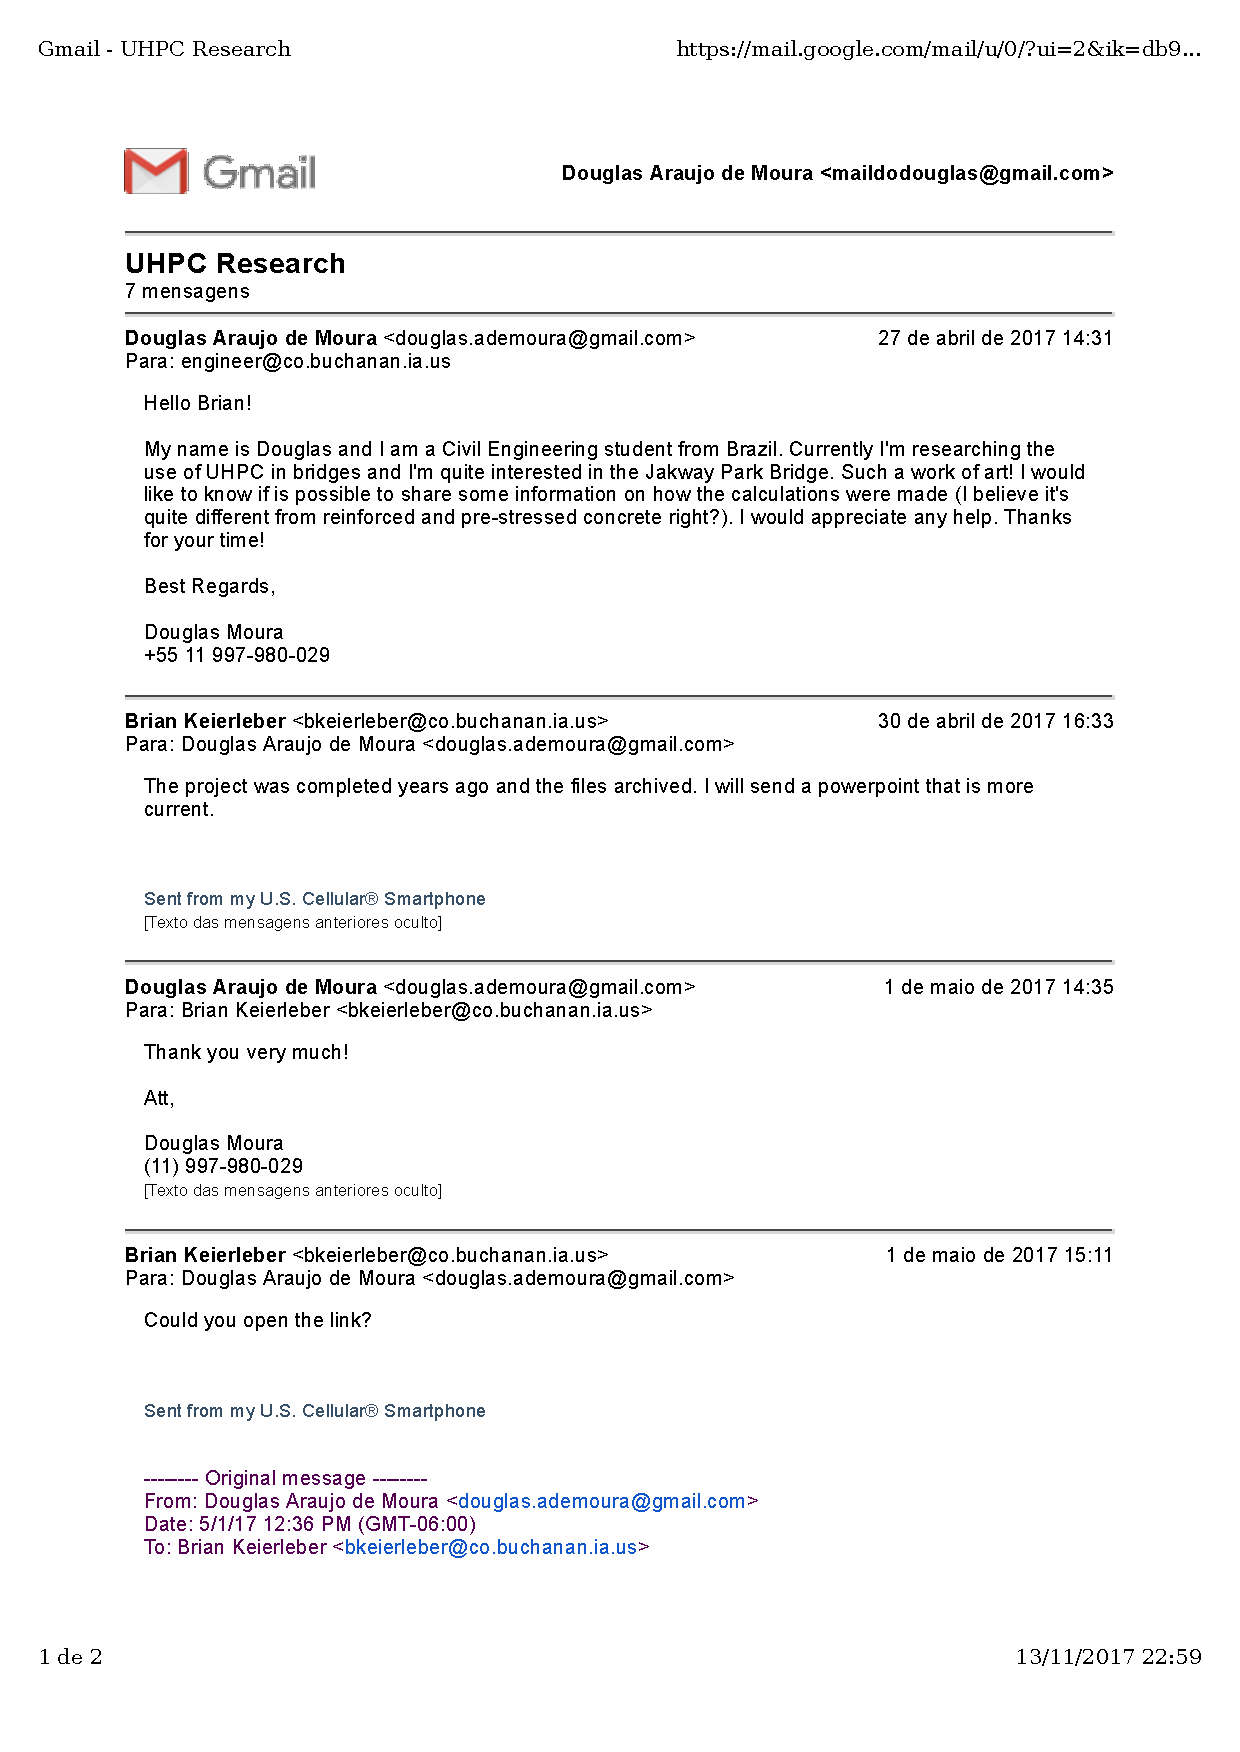
\includepdf[pages=-,pagecommand={},width=\textwidth]{anexos/brian.pdf}
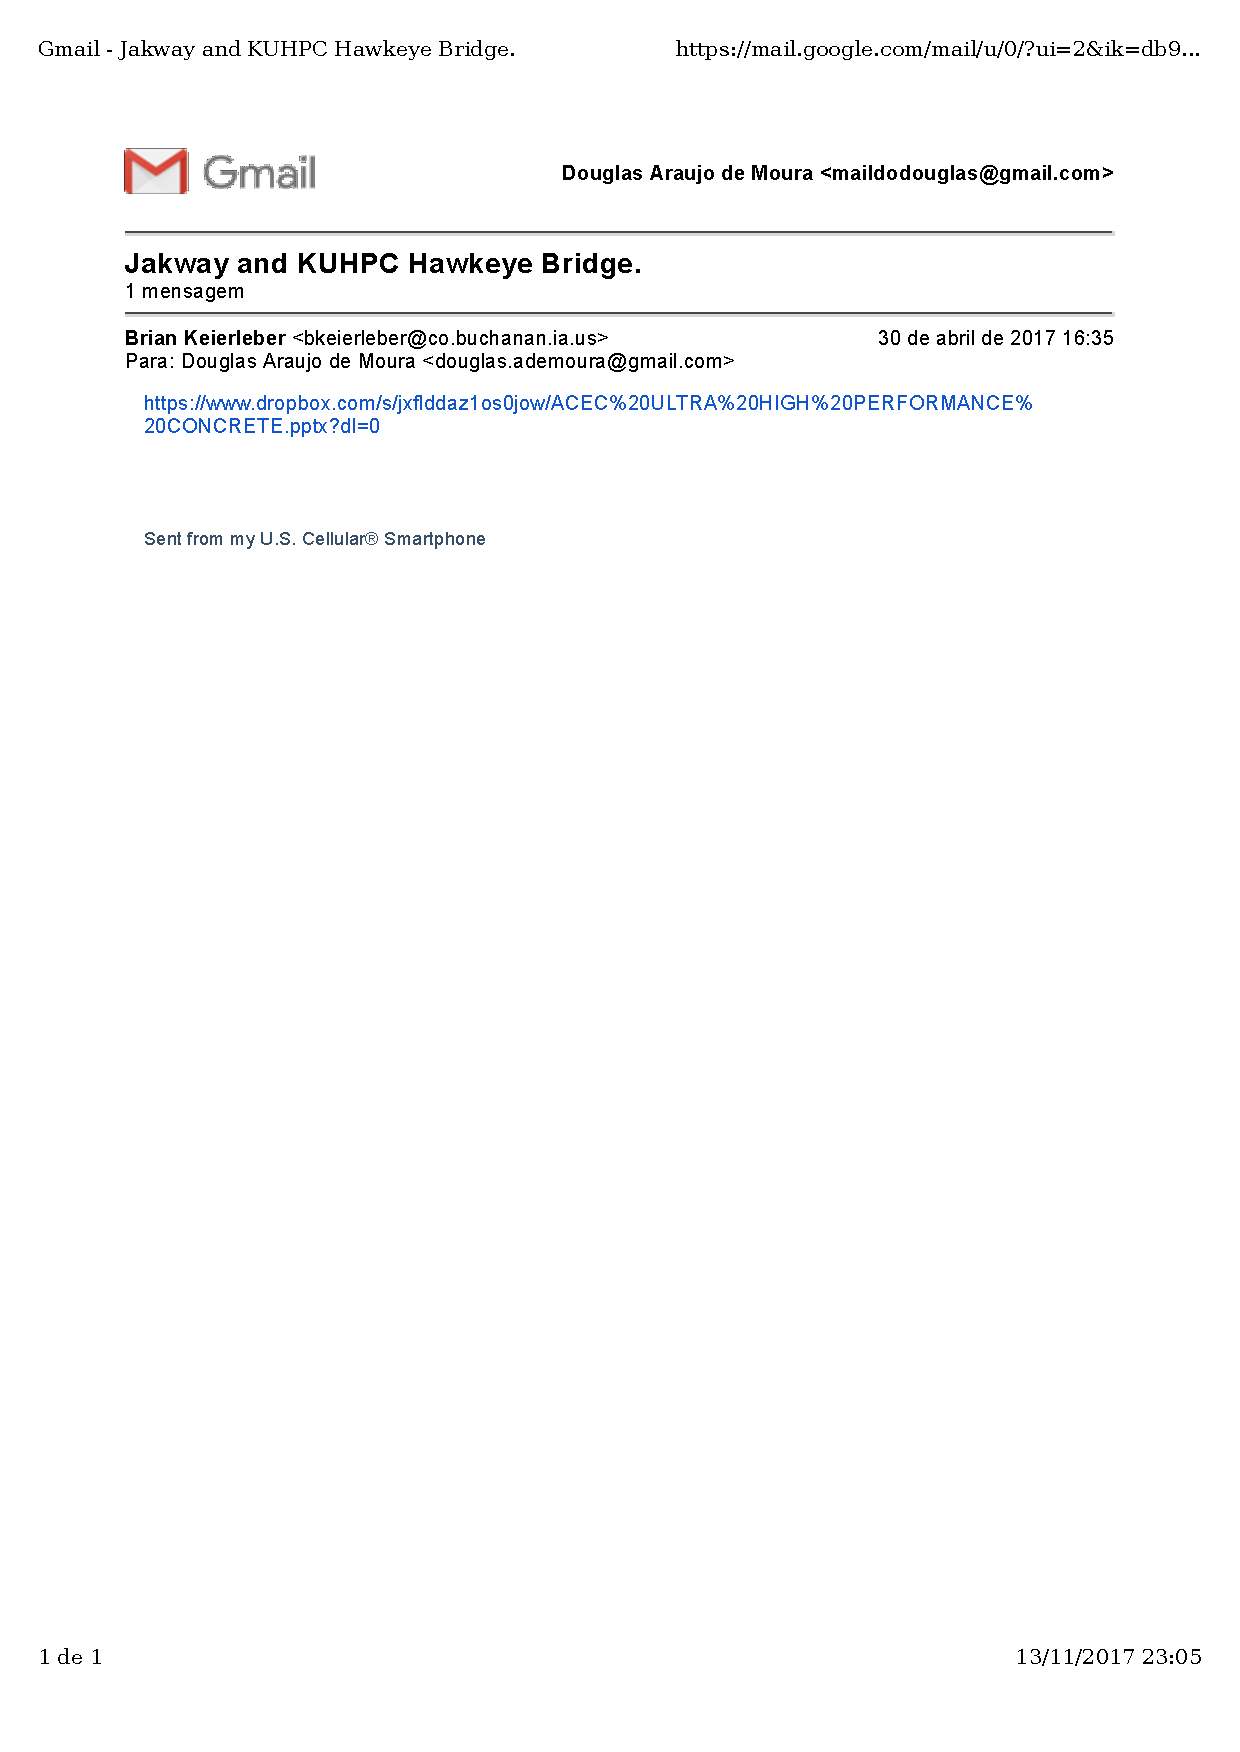
\includepdf[pages=-,pagecommand={},width=\textwidth]{anexos/link.pdf}

%
% ---
%\chapter{Tabelas da ABNT}\label{anexo:tabelasABNT}
% ---
%\begin{figure}[htb]
%	\caption{\label{classe-agressividade-ambiental}Tabela de classes de agressividade ambiental.}
%	\begin{center}
%	    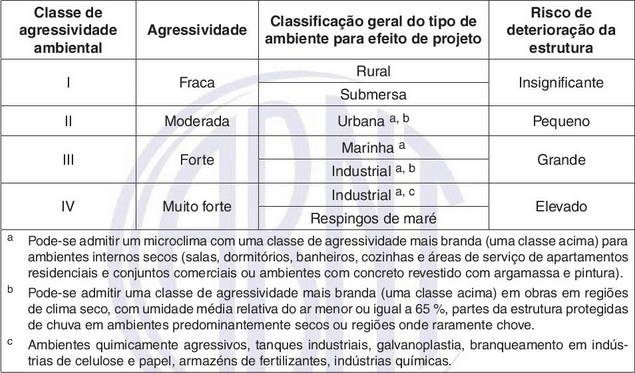
\includegraphics[max width=\textwidth]{classe-agressividade-ambiental.png}
%	\end{center}
%	\legend{Fonte: NBR 6118 \cite[p.~17]{NBR6118:2014}}
%\end{figure}
%
%\begin{figure}[htb]
%	\caption{\label{qualidade-do-concreto}Tabela da correspondência entre a classe de agressividade e a qualidade do concreto.}
%	\begin{center}
%	    \includegraphics[max width=\textwidth]{qualidade-do-concreto.png}
%	\end{center}
%	\legend{Fonte: NBR 6118 \cite[p.~18]{NBR6118:2014}}
%\end{figure}
%
%\begin{figure}[htb]
%	\caption{\label{cobrimento-nominal}Tabela da correspondência entre classe de agressividade ambiental e o cobrimento nominal para $\Delta$c = 10mm.}
%	\begin{center}
%	    \includegraphics[max width=\textwidth]{cobrimento-nominal.png}
%	\end{center}
%	\legend{Fonte: NBR 6118 \cite[p.~20]{NBR6118:2014}}
%\end{figure}
%
\end{anexosenv}

%---------------------------------------------------------------------
% INDICE REMISSIVO
%---------------------------------------------------------------------
\phantompart
\printindex
%---------------------------------------------------------------------

\end{document}